% =====================================================================
%  Anatomía de un LLM — Fase IV — Módulo 18
%  Arquitecturas modernas
%  Compilar: latexmk -r ../latexmkrc M18-arquitecturas.tex
% =====================================================================
\documentclass[11pt,a4paper,twoside,openany]{book}
\usepackage{../estilo-apuntes}

\newcommand{\ApuntesCurso}{Anatomía de un LLM}
\newcommand{\ApuntesModulo}{Módulo 18}

% Notación propia del módulo
\newcommand{\T}{^{\top}}
\newcommand{\uno}{\mathbf{1}}
\newcommand{\diag}{\operatorname{diag}}
\newcommand{\RMS}{\operatorname{RMS}}
\newcommand{\RMSNorm}{\operatorname{RMSNorm}}
\newcommand{\LN}{\operatorname{LN}}
\newcommand{\FFN}{\operatorname{FFN}}
\newcommand{\Attn}{\operatorname{Attn}}
\newcommand{\SwiGLU}{\operatorname{SwiGLU}}
\newcommand{\SiLU}{\operatorname{SiLU}}
\newcommand{\TopK}{\operatorname{TopK}}
\newcommand{\softplus}{\operatorname{softplus}}
\newcommand{\RoPE}{\operatorname{RoPE}}
\newcommand{\Lbal}{\mathcal{L}_{\mathrm{bal}}}
\newcommand{\dff}{d_{\mathrm{ff}}}
\newcommand{\dhd}{d_{h}}
\newcommand{\nkv}{n_{\mathrm{kv}}}
\newcommand{\dc}{d_{c}}
\newcommand{\Abar}{\bar{A}}
\newcommand{\Bbar}{\bar{B}}
\newcommand{\Icrit}{I^{\ast}}
\newcommand{\Nact}{N_{\mathrm{act}}}
\newcommand{\Ntot}{N_{\mathrm{tot}}}
\makeatletter\g@addto@macro\UrlBreaks{\do\-}\makeatother

\hypersetup{pdftitle={Módulo 18. Arquitecturas modernas},pdfauthor={Anatomía de un LLM}}

\begin{document}
\frontmatter
% ------------------------------------------------------------------ Portada
\begin{titlepage}
\centering
\vspace*{2.5cm}
{\large\scshape Anatomía de un LLM}\par
\vspace{0.4cm}
{\normalsize Fundamentos matemáticos de los modelos de lenguaje}\par
\vspace{2.2cm}
\rule{\textwidth}{0.8pt}\par\vspace{0.5cm}
{\small\scshape Fase IV \textperiodcentered\ Escala, sistemas y arquitecturas modernas}\par\vspace{0.3cm}
{\Huge\bfseries Módulo 18\par}\vspace{0.3cm}
{\LARGE Arquitecturas modernas\par}
\vspace{0.2cm}
{\large Normalización, atención eficiente, contexto largo, mezcla de expertos, modelos de espacio de estados y multimodalidad\par}
\vspace{0.5cm}\rule{\textwidth}{0.4pt}\par
\vspace{1.6cm}
{\large Apuntes del curso}\par
\vfill
{\small Edición de octubre de 2026}\par
\end{titlepage}

% ------------------------------------------------------- Presentación
\chapter*{Presentación del módulo}
\addcontentsline{toc}{chapter}{Presentación del módulo}
\markboth{Presentación del módulo}{}

El Transformer de los módulos~13 a~15 gasta el mismo cómputo en cada token, guarda durante la generación las claves y los valores de todas las posiciones anteriores y solo procesa texto. Los modelos de lenguaje publicados desde 2023 conservan su estructura, pero modifican casi todas sus piezas para reducir el coste por token, la memoria de inferencia o la dependencia cuadrática de la longitud del contexto. En marzo de 2024 xAI publicó los pesos de Grok-1, un modelo de unos $3{,}1\cdot 10^{11}$ parámetros que, sin embargo, usa solo una cuarta parte de ellos en cada token; el informe técnico de Gemini~1.5 lo describe como un Transformer de mezcla de expertos dispersa que procesa contextos de millones de tokens con texto, audio y vídeo intercalados. Este módulo estudia, con la notación y el rigor de los anteriores, los mecanismos que hacen posibles esas cifras: las componentes de consenso del bloque moderno, las variantes de la atención que reducen la caché de claves y valores, la atención local y la extensión del contexto, la mezcla de expertos, los modelos de espacio de estados y la representación de imágenes y audio como tokens. Sobre Claude, Gemini y Grok solo se usa información pública; cuando un dato no lo es, se indica.

\section*{Objetivos}
Al finalizar el módulo, el estudiante debe ser capaz de:
\begin{enumerate}[label=\arabic*.]
  \item describir el bloque Transformer de consenso (pre-norm, RMSNorm, SwiGLU, RoPE, sin sesgos), demostrar las propiedades de invariancia de RMSNorm y justificar los hiperparámetros de forma habituales;
  \item calcular la memoria de la caché de claves y valores con MHA, GQA, MQA y MLA, demostrar que la decodificación con MHA tiene intensidad aritmética constante y explicar la absorción de matrices de MLA;
  \item definir la atención con ventana deslizante, demostrar la fórmula de su campo receptivo y la corrección de la caché circular, y analizar la interpolación de posiciones, el cambio de base NTK y YaRN para extender el contexto de RoPE;
  \item formular una capa de mezcla de expertos con enrutado top-$k$, distinguir parámetros totales y activos, demostrar las cotas de la pérdida de balanceo y reconstruir los recuentos publicados de Mixtral y Grok-1;
  \item discretizar un modelo de espacio de estados, demostrar la equivalencia entre su forma recurrente y convolucional, la conexión del modelo selectivo de Mamba con una puerta recurrente y la asociatividad que permite el barrido paralelo;
  \item explicar cómo un Vision Transformer y un modelo de voz convierten imágenes y audio en secuencias de vectores y calcular el número de tokens y el coste resultantes.
\end{enumerate}

\section*{Requisitos previos}
Del módulo~2, el producto de matrices y la factorización de bajo rango; del módulo~4, la regla de la cadena; del módulo~5, la desigualdad de Cauchy--Schwarz; del módulo~11, LayerNorm, RMSNorm y las conexiones residuales; del módulo~12, las redes recurrentes y sus puertas; del módulo~13, la atención escalada, la máscara causal y la atención multicabeza; del módulo~14, el bloque decoder-only, SwiGLU, RoPE (tema~4) y el recuento de parámetros y FLOPs; del módulo~16, la regla $C\approx 6ND$, y del módulo~17, el modelo \emph{roofline} y la intensidad crítica de la A100, $\Icrit\approx 156$~FLOP/byte en bf16. La caché de claves y valores se introduce aquí y se implementa en el módulo~19.

\section*{Organización}
\begin{center}\small
\begin{tabular}{@{}cll@{}}
\toprule
Tema & Contenido & Fuentes principales \\
\midrule
1 & Componentes de consenso del Transformer moderno & \cite{cs336}, \cite{rmsnorm}, \cite{shazeerglu}, \cite{llama3} \\
2 & Atención eficiente en memoria: caché KV, MQA, GQA y MLA & \cite{mqa}, \cite{gqa}, \cite{deepseekv2}, \cite{cs336} \\
3 & Atención local y contexto largo & \cite{mistral}, \cite{longformer}, \cite{pi}, \cite{yarn} \\
4 & Mezcla de expertos & \cite{shazeer2017}, \cite{switch}, \cite{mixtral}, \cite{deepseekv3} \\
5 & Modelos de espacio de estados & \cite{s4}, \cite{mamba}, \cite{mit6003}, \cite{cs25} \\
6 & Multimodalidad: imágenes y audio como tokens & \cite{vit}, \cite{whisper}, \cite{soundstream}, \cite{d2l} \\
\bottomrule
\end{tabular}
\end{center}

Cada tema termina con una lista de lecturas y con ejercicios graduados en tres niveles: $\star$ comprensión, $\star\star$ cálculo y $\star\star\star$ demostración. Los ejercicios marcados con \emph{Fuente} están adaptados de cursos y libros de texto universitarios; el enunciado se ha redactado de nuevo y, en algunos casos, se han cambiado los datos para que puedan resolverse a mano. Las soluciones completas, paso a paso, están en el \cref{ap:soluciones}.

\section*{Sobre las fuentes}
El texto es de redacción propia. La organización sigue el bloque de arquitecturas del curso CS336 de Stanford, «Language Modeling from Scratch»~\cite{cs336}: la clase~3 sobre arquitecturas e hiperparámetros, la clase~4 sobre mezcla de expertos y la parte de la clase~10 (inferencia) dedicada a reducir la caché de claves y valores y a las alternativas al Transformer. Se complementa con el seminario CS25 de Stanford~\cite{cs25}, en particular la sesión de A.~Gu sobre modelos de espacio de estados, y con los temarios de los cursos CMU 11-711 (\emph{Advanced NLP})~\cite{cmu11711} y CMU 11-868 (\emph{Large Language Model Systems})~\cite{cmu11868}. Los métodos se toman de sus artículos originales: Zhang y Sennrich~\cite{rmsnorm} para RMSNorm, Shazeer~\cite{shazeerglu} para las unidades con puerta, Su \emph{et al.}~\cite{roformer} para RoPE, Shazeer~\cite{mqa} para MQA, Ainslie \emph{et al.}~\cite{gqa} para GQA, DeepSeek-AI~\cite{deepseekv2,deepseekv3} para MLA y DeepSeekMoE, Jiang \emph{et al.}~\cite{mistral} para la ventana deslizante, Beltagy \emph{et al.}~\cite{longformer} para Longformer, Chen \emph{et al.}~\cite{pi} y Peng \emph{et al.}~\cite{yarn} para la extensión del contexto, Shazeer \emph{et al.}~\cite{shazeer2017}, Fedus \emph{et al.}~\cite{switch} y Jiang \emph{et al.}~\cite{mixtral} para la mezcla de expertos, Gu \emph{et al.}~\cite{s4} y Gu y Dao~\cite{mamba} para los modelos de espacio de estados, Dosovitskiy \emph{et al.}~\cite{vit} para el Vision Transformer y Radford \emph{et al.}~\cite{whisper} para Whisper. Las configuraciones de Llama~2 y Llama~3 proceden de sus informes técnicos~\cite{llama2,llama3}, y las de Grok-1, del archivo \texttt{README} y del código publicados por xAI~\cite{grok1}. Los ejercicios universitarios proceden de la tarea~1 y de las clases de CS336~\cite{cs336a1,cs336}, del curso 6.003 del MIT~\cite{mit6003} y del libro \emph{Dive into Deep Learning}~\cite{d2l}. Sobre Claude no se usa ningún dato de arquitectura, porque Anthropic no lo ha publicado; sobre Gemini, solo el informe técnico~\cite{gemini15}, y sobre Grok, solo la versión de pesos abiertos~\cite{grok1}.

\section*{Notación}
\begin{center}\small
\begin{tabularx}{\textwidth}{@{}l>{\raggedright\arraybackslash}X@{}}
\toprule
Símbolo & Significado \\
\midrule
$d$, $L$, $\dff$ & dimensión del modelo, número de bloques y dimensión intermedia del MLP \\
$H$, $\dhd=d/H$ & cabezas de consulta y dimensión por cabeza \\
$\nkv$, $G$ & cabezas de clave y valor; número de grupos de GQA ($\nkv=G$) \\
$T$, $b$, $s$ & longitud de la secuencia, tamaño del lote y bytes por número (2 en bf16) \\
$\dc$, $d_h^{R}$ & dimensión latente de MLA y dimensión de la clave con RoPE desacoplada \\
$W$ & tamaño de la ventana de atención local \\
$\theta_i$, $\lambda_i=2\pi/\theta_i$, $\beta_0$ & frecuencias y longitudes de onda de RoPE; base ($10^{4}$ en el artículo original) \\
$s_{\mathrm{e}}=L'/L_0$ & factor de extensión del contexto, de $L_0$ a $L'$ tokens \\
$E_1,\dots,E_N$, $k$ & expertos y número de expertos activos por token \\
$z=xW_r$, $p_i(x)$, $g_i(x)$ & logits del enrutador, probabilidades y pesos de combinación \\
$f_i$, $P_i$, $\Lbal$ & fracción de tráfico, probabilidad media y pérdida de balanceo del experto $i$ \\
$\Ntot$, $\Nact$ & parámetros totales y activos por token \\
$A,B,C$, $\Delta$ & matrices de un modelo de espacio de estados continuo y paso de discretización \\
$\Abar,\Bbar$, $h_t$ & matrices discretizadas y estado en el instante $t$ \\
$\sigma$, $\softplus(z)=\ln(1+e^{z})$ & sigmoide logística y función \emph{softplus} \\
$P$, $C_{\mathrm{in}}$ & lado del parche de un ViT y número de canales de la imagen \\
\bottomrule
\end{tabularx}
\end{center}

Como en el módulo~14, los vectores de tokens son filas y una capa lineal actúa como $x\mapsto xW$. Los números grandes se escriben con espacio fino como separador de miles ($46\,702\,792\,704$). Las unidades binarias son $1$~KiB $=2^{10}$, $1$~MiB $=2^{20}$ y $1$~GiB $=2^{30}$~bytes; 1~GB son $10^{9}$~bytes.

\tableofcontents

\mainmatter
% =====================================================================
\chapter{Componentes de consenso del Transformer moderno}
\label{tema:1}
% =====================================================================

Entre el Transformer original de 2017 y los modelos abiertos actuales hay decenas de variantes publicadas, pero la mayoría converge en un mismo bloque: normalización antes de cada subcapa, RMSNorm, MLP con puerta, codificación rotatoria de la posición y ausencia de sesgos. Este tema define ese bloque de consenso, demuestra las propiedades de RMSNorm que lo justifican y estudia los hiperparámetros de forma que comparten casi todos los modelos. Se sigue la clase~3 del curso CS336~\cite{cs336}, el artículo de Zhang y Sennrich~\cite[§3--4]{rmsnorm}, el de Shazeer~\cite[§2--3]{shazeerglu} y la tabla de hiperparámetros de Llama~3~\cite[§3.2]{llama3}. El bloque decoder-only, SwiGLU y RoPE ya se han estudiado en el módulo~14; aquí se recuerdan solo en la medida en que se necesitan.

\section{El bloque de consenso}

La clase~3 de CS336 compara las arquitecturas densas publicadas entre 2019 y 2025 y observa que hay poco consenso en los detalles, con una excepción casi universal: la normalización se coloca a la entrada de cada subcapa, fuera del camino residual~\cite{cs336}. Las demás elecciones convergen hacia lo que el curso llama arquitecturas «de tipo LLaMA».

\begin{definicion}[Bloque de consenso]\label{def:consenso}
Sean $h\in\R^{1\times d}$ la fila de un token en el flujo residual, $\Attn$ una atención multicabeza causal con RoPE y $\FFN$ un MLP SwiGLU sin sesgos. El \emph{bloque de consenso} es
\[
a=h+\Attn\bigl(\RMSNorm_1(h)\bigr),\qquad h'=a+\FFN\bigl(\RMSNorm_2(a)\bigr),
\]
donde las capas lineales no tienen sesgo y la posición se introduce solo mediante la rotación de consultas y claves en cada capa. El modelo completo añade un $\RMSNorm$ final antes de la matriz de salida.
\end{definicion}

\begin{table}[ht]
\centering\small
\caption{Elecciones de arquitectura del Transformer original y de Llama~3. Fuentes: \cite[§3]{vaswani}, \cite[§3.2 y tabla~3]{llama3} y \cite{cs336}.}\label{tab:consenso}
\begin{tabular}{@{}lll@{}}
\toprule
Elección & Transformer (2017) & Llama~3 (2024) \\
\midrule
Posición de la normalización & tras la subcapa (post-norm) & antes de la subcapa (pre-norm) \\
Normalización & LayerNorm & RMSNorm \\
Activación del MLP & ReLU, $\dff=4d$ & SwiGLU, $\dff\approx 3{,}5d$ \\
Posición & sinusoidal sumada a la entrada & RoPE en cada capa, base $5\cdot 10^{5}$ \\
Sesgos & sí & no \\
Atención & multicabeza (MHA) & agrupada (GQA, 8 cabezas K/V) \\
\bottomrule
\end{tabular}
\end{table}

\begin{observacion}
Las justificaciones de cada elección son mayoritariamente empíricas. Shazeer termina su artículo sobre las unidades con puerta sin ofrecer explicación de por qué funcionan mejor~\cite[§4]{shazeerglu}, y la clase~3 de CS336 insiste en que las diferencias entre variantes son pequeñas y en que el argumento a favor de RMSNorm es sobre todo de coste~\cite{cs336}. Lo que sí admite demostración son las propiedades algebraicas que diferencian unas variantes de otras, y a ellas se dedica la sección siguiente.
\end{observacion}

\section{RMSNorm}

\begin{definicion}[LayerNorm y RMSNorm]\label{def:rmsnorm}
Sean $x\in\R^{d}$, $\gamma\in\R^{d}$ un vector de ganancias y $\varepsilon\ge 0$. Con $\mu(x)=\frac1d\sum_i x_i$ y $\RMS_\varepsilon(x)=\sqrt{\frac1d\sum_i x_i^{2}+\varepsilon}$, se definen
\[
\RMSNorm(x)=\frac{x}{\RMS_\varepsilon(x)}\odot\gamma,\qquad
\LN(x)=\frac{x-\mu(x)\uno}{\sqrt{\frac1d\sum_i(x_i-\mu(x))^{2}+\varepsilon}}\odot\gamma+\beta,
\]
donde $\odot$ es el producto componente a componente y $\beta\in\R^{d}$ es el sesgo de LayerNorm. RMSNorm no resta la media ni tiene sesgo~\cite[§4, ec.~4]{rmsnorm}.
\end{definicion}

La práctica~1 de CS336 usa exactamente esta forma, con $\varepsilon=10^{-5}$ y cálculo en fp32 aunque la entrada esté en bf16, para evitar desbordamientos al elevar al cuadrado~\cite[§3.4.1]{cs336a1}.

\begin{proposicion}[Propiedades de RMSNorm]\label{prop:rmsnorm}
Sea $\varepsilon=0$ y sea $x\ne 0$.
\begin{enumerate}
  \item \emph{Norma fija.} Con $\gamma=\uno$, $\norm{\RMSNorm(x)}=\sqrt d$.
  \item \emph{Invariancia de escala.} Para todo $\alpha>0$, $\RMSNorm(\alpha x)=\RMSNorm(x)$; para $\alpha<0$, $\RMSNorm(\alpha x)=-\RMSNorm(x)$.
  \item \emph{Invariancia ante la escala de los pesos.} Si $x=uW$ es la salida de una capa lineal y $W$ se sustituye por $\alpha W$ con $\alpha>0$, la salida normalizada no cambia.
  \item \emph{Relación con LayerNorm.} Con $\beta=0$, $\LN(x)=\RMSNorm\bigl(x-\mu(x)\uno\bigr)$ siempre que $x$ no sea constante.
\end{enumerate}
\end{proposicion}

\begin{proof}
(i) $\norm{x/\RMS(x)}^{2}=\sum_i x_i^{2}\big/\bigl(\frac1d\sum_i x_i^{2}\bigr)=d$.

(ii) $\RMS(\alpha x)=\sqrt{\frac1d\sum_i\alpha^{2}x_i^{2}}=\abs{\alpha}\RMS(x)$, luego $\alpha x/\RMS(\alpha x)=(\alpha/\abs{\alpha})\,x/\RMS(x)$, y $\alpha/\abs{\alpha}=\pm1$ según el signo de $\alpha$.

(iii) $u(\alpha W)=\alpha\,(uW)=\alpha x$, y basta aplicar (ii).

(iv) Sea $c=x-\mu(x)\uno$, que no es nulo porque $x$ no es constante. Como $\mu(c)=0$, el denominador de LayerNorm es $\sqrt{\frac1d\sum_i c_i^{2}}=\RMS(c)$, y $\LN(x)=c/\RMS(c)\odot\gamma=\RMSNorm(c)$.
\end{proof}

La \cref{prop:rmsnorm}(iv) dice que LayerNorm es RMSNorm precedida de un centrado. Lo que RMSNorm pierde es, por tanto, la invariancia ante traslaciones: $\LN(x+t\uno)=\LN(x)$ para todo $t\in\R$, mientras que $\RMSNorm(x+t\uno)\ne\RMSNorm(x)$ en general. Zhang y Sennrich conjeturan que la invariancia ante la escala es la propiedad que importa para la estabilidad, y no la de centrado, y la tabla~1 de su artículo compara ambas normalizaciones en estos términos~\cite[§4.1]{rmsnorm}.

\begin{ejemplo}[RMSNorm frente a LayerNorm]\label{ej:rmsnorm}
Sea $x=(1,2,3,-2)$ con $\gamma=\uno$, $\beta=0$ y $\varepsilon=0$. Entonces $\sum_i x_i^{2}=18$, $\RMS(x)=\sqrt{18/4}=2{,}121$ y
\[
\RMSNorm(x)=(0{,}4714;\ 0{,}9428;\ 1{,}414;\ -0{,}9428),
\]
cuya norma es $2=\sqrt 4$. Para LayerNorm, $\mu(x)=1$, el vector centrado es $c=(0,1,2,-3)$, con $\sum_i c_i^{2}=14$ y $\RMS(c)=\sqrt{3{,}5}=1{,}871$, y
\[
\LN(x)=(0;\ 0{,}5345;\ 1{,}069;\ -1{,}604).
\]
Las dos salidas difieren porque la media de $x$ no es nula; si se duplica $x$, ninguna de las dos cambia.
\end{ejemplo}

\begin{observacion}[Coste]
Las normalizaciones suponen una fracción despreciable de los FLOPs de un bloque, pero no de su tiempo: son operaciones limitadas por la memoria, con intensidad aritmética baja (módulo~17, tema~2). Por eso la clase~3 de CS336 atribuye a RMSNorm una ganancia de tiempo real apreciable a pesar de ahorrar muy pocas operaciones~\cite{cs336}, y Zhang y Sennrich informan de reducciones del tiempo de ejecución de entre el 7 y el 64\,\% según el modelo~\cite{rmsnorm}.
\end{observacion}

\section{El presupuesto del MLP con puerta}

\begin{definicion}[MLP SwiGLU]\label{def:swiglu}
Sean $W_1,W_3\in\R^{d\times\dff}$ y $W_2\in\R^{\dff\times d}$. El MLP SwiGLU es
\[
\FFN_{\SwiGLU}(x)=\bigl(\SiLU(xW_1)\odot xW_3\bigr)W_2,\qquad \SiLU(t)=t\,\sigma(t),
\]
sin sesgos~\cite[ec.~6]{shazeerglu}.
\end{definicion}

\begin{proposicion}[Presupuesto de parámetros]\label{prop:presupuesto}
Un MLP SwiGLU con dimensión intermedia $\dff$ tiene $3d\,\dff$ parámetros y cuesta $6d\,\dff$ FLOPs por token en la pasada hacia delante. Tiene los mismos parámetros y FLOPs que un MLP de dos matrices con dimensión intermedia $4d$ si y solo si $\dff=\frac83 d$.
\end{proposicion}

\begin{proof}
Cada una de las tres matrices tiene $d\,\dff$ entradas, y cada producto de una fila por una matriz $d\times\dff$ (o $\dff\times d$) cuesta $2d\,\dff$ FLOPs (módulo~14, tema~6). El MLP de dos matrices con $4d$ tiene $2\cdot d\cdot 4d=8d^{2}$ parámetros. La igualdad $3d\,\dff=8d^{2}$ equivale a $\dff=8d/3$; el argumento para los FLOPs es idéntico, con un factor~2 en ambos miembros.
\end{proof}

Shazeer aplica esta regla en sus experimentos: compara un MLP con $\dff=3072$ y dos matrices con variantes con puerta de $\dff=2048=\frac23\cdot 3072$~\cite[§3.1]{shazeerglu}. La clase~3 de CS336 recoge que la mayoría de los modelos con puerta usan cocientes $\dff/d$ entre $2{,}5$ y $3{,}5$, y que fuera de ese intervalo hay excepciones como T5, con un cociente de~64~\cite{cs336}. La \cref{tab:hiper} muestra los valores de Llama~3, Mixtral y Grok-1.

\begin{table}[ht]
\centering\small
\caption{Hiperparámetros de forma de modelos con publicación de su configuración. Fuentes: \cite[tabla~3]{llama3}, \cite[tabla~1]{mixtral} y el archivo \texttt{run.py} de~\cite{grok1}.}\label{tab:hiper}
\begin{tabular}{@{}lrrrrrrr@{}}
\toprule
Modelo & $L$ & $d$ & $\dff$ & $H$ & $\nkv$ & $\dff/d$ & $d/L$ \\
\midrule
Llama~3 8B & 32 & 4096 & 14\,336 & 32 & 8 & $3{,}5$ & 128 \\
Llama~3 70B & 80 & 8192 & 28\,672 & 64 & 8 & $3{,}5$ & $102{,}4$ \\
Llama~3 405B & 126 & 16\,384 & 53\,248 & 128 & 8 & $3{,}25$ & $130{,}0$ \\
Mixtral 8x7B & 32 & 4096 & 14\,336 & 32 & 8 & $3{,}5$ & 128 \\
Grok-1 & 64 & 6144 & 32\,768 & 48 & 8 & $5{,}333$ & 96 \\
\bottomrule
\end{tabular}
\end{table}

\section{Hiperparámetros de forma}

La clase~3 de CS336 identifica tres regularidades más, todas ellas con excepciones documentadas~\cite{cs336}.

\begin{definicion}[Hiperparámetros de forma]\label{def:forma}
En un Transformer con $L$ bloques, dimensión $d$ y $H$ cabezas de dimensión $\dhd$:
\begin{enumerate}
  \item la \emph{regla de las cabezas} es $H\dhd=d$;
  \item la \emph{relación de aspecto} es $r=d/L$;
  \item el \emph{tamaño del vocabulario} es $\abs{\V}$.
\end{enumerate}
\end{definicion}

Los modelos de la \cref{tab:hiper} cumplen la regla de las cabezas con $\dhd=128$, salvo Grok-1, en el que $48\cdot 128=6144=d$ también la cumple. La clase de CS336 sitúa la relación de aspecto de la mayoría de los modelos entre 100 y 200, y los vocabularios entre $3\cdot 10^{4}$ y $5\cdot 10^{4}$ tokens para modelos monolingües y entre $10^{5}$ y $2{,}5\cdot 10^{5}$ para los multilingües: Llama~2 usa $32\,000$ y Llama~3, unos $128\,000$~\cite{cs336,llama3}.

\begin{proposicion}[Dimensión a partir del tamaño y la relación de aspecto]\label{prop:aspecto}
Sea un Transformer de consenso con $\dff=\frac83 d$ y atención multicabeza, cuyos bloques contienen $N_{\mathrm{b}}$ parámetros en total, y sea $r=d/L$ su relación de aspecto. Despreciando las normalizaciones, $N_{\mathrm{b}}=12Ld^{2}$ y, por tanto,
\[
d=\Bigl(\frac{rN_{\mathrm{b}}}{12}\Bigr)^{1/3},\qquad L=\frac dr .
\]
\end{proposicion}

\begin{proof}
La atención tiene cuatro matrices $d\times d$, es decir, $4d^{2}$ parámetros; el MLP, $3d\,\dff=8d^{2}$ por la \cref{prop:presupuesto}. Cada bloque tiene $12d^{2}$ parámetros y $L$ bloques, $12Ld^{2}$. Sustituyendo $L=d/r$, $N_{\mathrm{b}}=12d^{3}/r$, y se despeja $d$.
\end{proof}

\begin{ejemplo}[Forma de un modelo de $4\cdot 10^{11}$ parámetros]\label{ej:aspecto}
Con $N_{\mathrm{b}}=4{,}05\cdot 10^{11}$ y $r=130$, la \cref{prop:aspecto} da $d=(130\cdot 4{,}05\cdot 10^{11}/12)^{1/3}=(4{,}388\cdot 10^{12})^{1/3}=16\,371$ y $L=16\,371/130=125{,}9$. Llama~3 405B tiene $d=16\,384$ y $L=126$ (\cref{tab:hiper}). La coincidencia es en parte casual, porque Llama~3 usa GQA y $\dff=3{,}25d$, pero muestra que dos números bastan para fijar la forma de un modelo.
\end{ejemplo}

\begin{observacion}[Estabilidad]
La clase~3 de CS336 recoge tres recursos de estabilidad frecuentes en modelos recientes, todos dirigidos a las funciones softmax: la pérdida auxiliar $z$ sobre el logaritmo del denominador de la softmax de salida, la normalización de consultas y claves antes del producto escalar (\emph{QK-norm}) y el recorte suave de los logits mediante una tangente hiperbólica~\cite{cs336}. Las tres limitan el crecimiento de los logits, cuyo exceso satura la softmax y desestabiliza el entrenamiento.
\end{observacion}

\begin{lecturas}
\item Stanford CS336~\cite{cs336}, clase~3, «Architectures, hyperparameters»: comparación de arquitecturas y tablas de hiperparámetros.
\item Zhang y Sennrich~\cite{rmsnorm}, §4 «RMSNorm» y §4.1 «Invariance Analysis».
\item Shazeer~\cite{shazeerglu}, §2 «Gated Linear Units (GLU) and Variants» y §3.1.
\item Grattafiori \emph{et al.}~\cite{llama3}, §3.2 «Model Architecture» y tabla~3.
\item Tarea~1 de CS336~\cite{cs336a1}, §3.4.1 (RMSNorm) y §7.3 (ablaciones de arquitectura).
\end{lecturas}

\section*{Ejercicios del tema 1}
\addcontentsline{toc}{section}{Ejercicios del tema 1}

\begin{ejercicio}{1}{eje:1-vf}
Justifique si son verdaderas o falsas: (a) RMSNorm es invariante ante la suma de una constante a todas las componentes; (b) un MLP SwiGLU con $\dff=4d$ tiene un 50\,\% más de parámetros que un MLP ReLU con $\dff=4d$; (c) en todos los modelos de la \cref{tab:hiper} se cumple $H\dhd=d$.
\end{ejercicio}

\begin{ejercicio}{2}{eje:1-norm}
Sea $x=(2,-1,0,3)$, con $\gamma=\uno$, $\beta=0$ y $\varepsilon=0$. Calcule $\RMSNorm(x)$, $\LN(x)$ y $\RMSNorm(3x)$, y compruebe la \cref{prop:rmsnorm}(i).
\end{ejercicio}

\begin{ejercicio}{2}{eje:1-llama3}
Con los datos de la \cref{tab:hiper}, calcule para los tres modelos de Llama~3 la dimensión por cabeza, el número de cabezas de consulta que comparten cada cabeza de clave y valor, y los parámetros de un bloque (atención con GQA, SwiGLU y dos RMSNorm). ¿Qué fracción del bloque corresponde al MLP en el modelo 8B?
\end{ejercicio}

\begin{ejercicio}{2}{eje:1-swiglu}
En la ablación de la tarea~1 de CS336 se compara un MLP SwiGLU con $\dff\approx\frac83 d$, redondeado a un múltiplo de~64, con un MLP de dos matrices con activación SiLU y $\dff=4d$. Con $d=512$: (a) calcule el $\dff$ del SwiGLU redondeando $\frac83 d$ al múltiplo de~64 más próximo; (b) cuente los parámetros de ambos MLP; (c) calcule la diferencia relativa y explique por qué la comparación es justa.
\fuente{adaptado de la tarea~1 de CS336~\cite{cs336a1}, §7.3, problema \texttt{swiglu\_ablation}.}
\end{ejercicio}

\begin{ejercicio}{3}{eje:1-inv}
Demuestre que $\LN(x+t\uno)=\LN(x)$ para todo $t\in\R$ y toda $x$ no constante, y que RMSNorm no tiene esta propiedad: encuentre $x\in\R^{2}$ y $t$ con $\RMSNorm(x+t\uno)\ne\RMSNorm(x)$. Demuestre también que, si $\gamma=\uno$, la salida de RMSNorm determina $x$ salvo un factor positivo.
\end{ejercicio}

\begin{ejercicio}{3}{eje:1-aspecto}
(a) Generalice la \cref{prop:aspecto} a un MLP con $\dff=\rho d$ y atención con $\nkv$ cabezas de clave y valor de dimensión $\dhd=d/H$. (b) Aplique la fórmula de la \cref{prop:aspecto} a $N_{\mathrm{b}}=7\cdot 10^{10}$ y $r=102$, y compare con Llama~3 70B. (c) Recalcule los parámetros de los bloques de Llama~3 70B con la fórmula de (a) y explique la diferencia con (b).
\end{ejercicio}

% =====================================================================
\chapter{Atención eficiente en memoria: caché KV, MQA, GQA y MLA}
\label{tema:2}
% =====================================================================

Al generar texto, un Transformer produce un token cada vez y reutiliza las claves y los valores de las posiciones anteriores. Esa reutilización ahorra cómputo, pero obliga a guardar y a leer en cada paso una caché que crece con la longitud del contexto y con el tamaño del lote, y que en contextos largos ocupa más memoria que los propios pesos. Este tema cuantifica esa caché, demuestra que con atención multicabeza la decodificación está necesariamente limitada por la memoria y estudia las tres variantes que la reducen: la atención multiconsulta (MQA), la atención de consultas agrupadas (GQA) y la atención latente multicabeza (MLA). Se sigue a Shazeer~\cite[§2.4 y §3]{mqa}, a Ainslie \emph{et al.}~\cite[§2]{gqa}, a DeepSeek-AI~\cite[§2.1]{deepseekv2} y la clase~10 de CS336~\cite{cs336}.

\section{La caché de claves y valores}

Sea una capa de atención con $H$ cabezas de dimensión $\dhd$. En la generación autorregresiva, al procesar el token $t$ se necesitan las consultas de $t$ y las claves y los valores de las posiciones $1,\dots,t$. Por la causalidad (módulo~14, tema~1), las claves y los valores de las posiciones $j<t$ no dependen de $t$: se calculan una vez y se guardan.

\begin{definicion}[Caché KV]\label{def:cache}
La \emph{caché KV} de una capa, tras procesar $T$ tokens, es el par de tensores $(K,V)$ con las claves y los valores de las $T$ posiciones para cada una de las $\nkv$ cabezas de clave y valor. Cada tensor tiene $T\cdot\nkv\cdot\dhd$ números por secuencia.
\end{definicion}

\begin{proposicion}[Tamaño de la caché KV]\label{prop:cache}
Un modelo de $L$ capas con $\nkv$ cabezas de clave y valor de dimensión $\dhd$, que procesa un lote de $b$ secuencias de $T$ tokens con $s$ bytes por número, necesita
\[
M_{\mathrm{KV}}=2\,L\,\nkv\,\dhd\,T\,b\,s\ \text{bytes}.
\]
\end{proposicion}

\begin{proof}
Por la \cref{def:cache}, cada capa guarda $T\nkv\dhd$ números para $K$ y otros tantos para $V$, por secuencia. Se multiplica por $2$ (claves y valores), por $L$ capas, por $b$ secuencias y por $s$ bytes.
\end{proof}

\begin{ejemplo}[Llama~2 70B]\label{ej:llama2kv}
Llama~2 70B tiene $L=80$, $H=64$ cabezas de consulta de dimensión $\dhd=128$ y usa GQA con $\nkv=8$~\cite{llama2}. En bf16 ($s=2$), por token y secuencia, la caché ocuparía $2\cdot 80\cdot 64\cdot 128\cdot 2=2\,621\,440$~bytes $=2{,}5$~MiB con atención multicabeza ($\nkv=64$) y ocupa $327\,680$~bytes $=320$~KiB con GQA. Para $T=4096$ y $b=16$, eso son $160$~GiB frente a $20$~GiB. Los pesos en bf16 ocupan unos $140$~GB.
\end{ejemplo}

\section{La decodificación está limitada por la memoria}

El módulo~17 definió la intensidad aritmética de una operación como el cociente entre FLOPs y bytes transferidos, y la comparó con la intensidad crítica del acelerador. El paso de atención de la decodificación tiene una intensidad que no mejora con el lote.

\begin{proposicion}[Intensidad de la atención en la decodificación]\label{prop:intensidad}
Sea una capa con $H$ cabezas de consulta y $\nkv$ cabezas de clave y valor de dimensión $\dhd$, y sea un paso de decodificación de una secuencia cuyo contexto tiene $T$ posiciones. Contando solo los productos $q\,K\T$ y $a\,V$ y la lectura de la caché, la intensidad aritmética es
\[
I=\frac{2H}{s\,\nkv}\ \text{FLOP/byte},
\]
independiente de $T$ y del tamaño del lote. Con MHA ($\nkv=H$) en bf16, $I=1$.
\end{proposicion}

\begin{proof}
Para cada cabeza de consulta, el producto de $q\in\R^{1\times\dhd}$ por $K\T\in\R^{\dhd\times T}$ cuesta $2\dhd T$ FLOPs, y el de los pesos $a\in\R^{1\times T}$ por $V\in\R^{T\times\dhd}$, otros $2T\dhd$. Con $H$ cabezas: $F=4HT\dhd$. Los bytes leídos de la caché son $Q=2T\nkv\dhd s$, porque cada cabeza de clave y valor se lee una vez y la comparten las $H/\nkv$ consultas de su grupo. Entonces $I=F/Q=4HT\dhd/(2T\nkv\dhd s)=2H/(s\nkv)$. Con un lote de $b$ secuencias, $F$ y $Q$ se multiplican por $b$, porque cada secuencia tiene su propia caché, y el cociente no cambia.
\end{proof}

La intensidad crítica de la A100 en bf16 es $\Icrit\approx 156$~FLOP/byte (módulo~17, tema~2). Con MHA, la atención de la decodificación aprovecha menos del $1\,\%$ del cómputo disponible, y aumentar el lote no ayuda. Los productos de las matrices de pesos, en cambio, sí ganan intensidad con el lote, porque todas las secuencias comparten los mismos pesos. Shazeer llega a la misma conclusión con otro recuento: en la decodificación incremental con MHA, el cociente entre accesos a memoria y operaciones es $\Theta(n/d+1/b)$, y el término $n/d$, debido a la lectura de las claves y los valores, no disminuye con el lote~\cite[§2.4.1]{mqa}. Reducir $\nkv$ es la forma directa de atacarlo.

\section{Atención multiconsulta y de consultas agrupadas}

\begin{definicion}[MQA y GQA]\label{def:gqa}
Sea $H$ divisible por $G$. La \emph{atención de consultas agrupadas} con $G$ grupos (GQA-$G$) divide las $H$ cabezas de consulta en $G$ grupos de $H/G$ cabezas consecutivas; todas las cabezas de un grupo comparten una única cabeza de clave y una de valor~\cite[§2.2]{gqa}. Con proyecciones $W_Q^{(i)}\in\R^{d\times\dhd}$ para $i=1,\dots,H$ y $W_K^{(g)},W_V^{(g)}\in\R^{d\times\dhd}$ para $g=1,\dots,G$, la cabeza $i$ usa la clave y el valor del grupo $g(i)=\lceil iG/H\rceil$. El caso $G=1$ es la \emph{atención multiconsulta} (MQA)~\cite[§3]{mqa}, y el caso $G=H$ es la atención multicabeza.
\end{definicion}

\begin{proposicion}[Ahorro de GQA]\label{prop:gqa}
Con $\nkv=G$, respecto de MHA:
\begin{enumerate}
  \item la caché KV se divide exactamente por $H/G$;
  \item las proyecciones de clave y valor pasan de $2d^{2}$ a $2d\,G\dhd$ parámetros, y las de consulta y salida no cambian;
  \item la intensidad de la \cref{prop:intensidad} se multiplica por $H/G$.
\end{enumerate}
\end{proposicion}

\begin{proof}
(i) y (iii) se siguen de sustituir $\nkv=G$ en las \cref{prop:cache,prop:intensidad}. (ii) Con MHA hay $H$ proyecciones $d\times\dhd$ para $K$ y otras tantas para $V$, es decir, $2Hd\dhd=2d^{2}$ parámetros si $H\dhd=d$; con GQA hay $G$ de cada tipo, $2Gd\dhd$. Las consultas siguen teniendo $H$ cabezas y $W_O$ sigue siendo $d\times d$.
\end{proof}

\begin{figure}[ht]
\centering
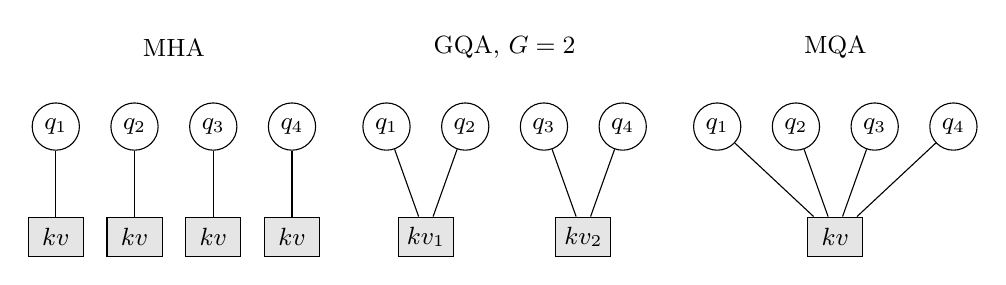
\begin{tikzpicture}[font=\small,q/.style={draw,circle,minimum size=6mm,inner sep=0pt},kv/.style={draw,rectangle,fill=black!10,minimum width=7mm,minimum height=5mm,inner sep=0pt}]
  \foreach \x/\lab in {0/MHA, 4.2/{GQA, $G=2$}, 8.4/MQA}{\node at (\x+1.5,2.4) {\lab};}
  % MHA
  \foreach \i in {0,1,2,3}{\node[q] (a\i) at (\i,1.4) {$q_{\the\numexpr\i+1}$}; \node[kv] (ak\i) at (\i,0) {$kv$}; \draw (a\i)--(ak\i);}
  % GQA
  \foreach \i in {0,1,2,3}{\node[q] (b\i) at (4.2+\i,1.4) {$q_{\the\numexpr\i+1}$};}
  \node[kv] (bk0) at (4.7,0) {$kv_1$}; \node[kv] (bk1) at (6.7,0) {$kv_2$};
  \draw (b0)--(bk0) (b1)--(bk0) (b2)--(bk1) (b3)--(bk1);
  % MQA
  \foreach \i in {0,1,2,3}{\node[q] (c\i) at (8.4+\i,1.4) {$q_{\the\numexpr\i+1}$};}
  \node[kv] (ck) at (9.9,0) {$kv$};
  \foreach \i in {0,1,2,3}{\draw (c\i)--(ck);}
\end{tikzpicture}
\caption{Cabezas de consulta y cabezas de clave y valor en MHA, GQA con dos grupos y MQA, con $H=4$.}
\label{fig:gqa}
\end{figure}

Shazeer observó que MQA reduce el tiempo de decodificación por token de 46 a 3,8~microsegundos en su experimento de traducción, con una pérdida de calidad pequeña pero apreciable~\cite[§4.2 y §4.3]{mqa}. Ainslie \emph{et al.} proponen GQA como término medio y muestran, además, que un modelo entrenado con MHA puede convertirse en uno con GQA sin entrenarlo desde cero: se promedian las proyecciones de clave y valor de las cabezas de cada grupo y se continúa el entrenamiento durante un $5\,\%$ de los pasos originales (\emph{uptraining})~\cite[§2.1 y §3.1]{gqa}. GQA con 8 grupos queda cerca de MHA en calidad y cerca de MQA en velocidad. Llama~2 la usa en sus modelos de 34B y 70B~\cite[tabla~1]{llama2}, y Llama~3, Mixtral y Grok-1 en todos sus tamaños (\cref{tab:hiper}).

\begin{ejemplo}[Grok-1]\label{ej:grokkv}
Grok-1 tiene $L=64$, $H=48$ cabezas de consulta y $\nkv=8$, con $\dhd=128$ y contexto máximo de 8192 tokens~\cite{grok1}. Por la \cref{prop:cache}, en bf16 la caché de una secuencia completa ocupa $2\cdot 64\cdot 8\cdot 128\cdot 8192\cdot 2=2^{31}$~bytes $=2$~GiB; con MHA serían $48/8=6$ veces más, $12$~GiB.
\end{ejemplo}

\section{Atención latente multicabeza}

GQA reduce la caché eliminando cabezas de clave y valor. MLA, introducida en DeepSeek-V2, conserva $H$ cabezas, pero guarda en la caché un único vector de baja dimensión por token del que se reconstruyen todas las claves y todos los valores~\cite[§2.1.2]{deepseekv2}.

\begin{definicion}[MLA sin codificación de posición]\label{def:mla}
Sean $\dc\ll H\dhd$, $W^{DKV}\in\R^{d\times\dc}$ y, para cada cabeza $i$, $W^{UK}_i,W^{UV}_i\in\R^{\dc\times\dhd}$ y $W^{Q}_i\in\R^{d\times\dhd}$. Para el token $t$ con entrada $h_t\in\R^{1\times d}$,
\[
c_t=h_tW^{DKV}\in\R^{1\times\dc},\qquad k_{t,i}=c_tW^{UK}_i,\qquad v_{t,i}=c_tW^{UV}_i,\qquad q_{t,i}=h_tW^{Q}_i .
\]
La caché guarda solo los vectores latentes $c_1,\dots,c_T$.
\end{definicion}

Guardar $c_t$ en lugar de $k_{t,i}$ y $v_{t,i}$ solo ahorra memoria si no hay que reconstruir explícitamente las claves y los valores en cada paso. La factorización lo evita.

\begin{proposicion}[Absorción de las proyecciones]\label{prop:absorcion}
Con la notación de la \cref{def:mla}, sean $\tilde q_{t,i}=q_{t,i}(W^{UK}_i)\T\in\R^{1\times\dc}$ y $a_{t,i,j}$ los pesos de atención de la cabeza $i$. Entonces
\[
q_{t,i}\,k_{j,i}\T=\tilde q_{t,i}\,c_j\T,\qquad \sum_{j\le t}a_{t,i,j}\,v_{j,i}=\Bigl(\sum_{j\le t}a_{t,i,j}\,c_j\Bigr)W^{UV}_i .
\]
En consecuencia, las puntuaciones y la salida de cada cabeza se calculan a partir de los $c_j$, sin formar $k_{j,i}$ ni $v_{j,i}$; además, $W^{UK}_i$ puede integrarse en la proyección de consulta y $W^{UV}_i$, en la de salida.
\end{proposicion}

\begin{proof}
$q_{t,i}k_{j,i}\T=q_{t,i}(c_jW^{UK}_i)\T=q_{t,i}(W^{UK}_i)\T c_j\T=\tilde q_{t,i}c_j\T$, por la regla de la traspuesta de un producto. Para la segunda igualdad, $\sum_j a_{t,i,j}c_jW^{UV}_i=(\sum_j a_{t,i,j}c_j)W^{UV}_i$ por la distributividad del producto de matrices. Por último, $\tilde q_{t,i}=h_t\bigl(W^{Q}_i(W^{UK}_i)\T\bigr)$, con $W^{Q}_i(W^{UK}_i)\T\in\R^{d\times\dc}$ fija, y la salida de la cabeza se multiplica después por el bloque $i$ de $W_O$, de modo que $W^{UV}_iW_O^{(i)}$ es también una matriz fija.
\end{proof}

\begin{observacion}[RoPE desacoplada]
La absorción falla con RoPE. Con vectores fila, la rotación de la posición $m$ actúa como $x\mapsto xR_m$, y $R_mR_n\T=R_{m-n}$ (es la versión traspuesta de la identidad del módulo~14, tema~4). Si la consulta y la clave se rotan, la puntuación es $q_{t,i}R_t(c_jW^{UK}_iR_j)\T=q_{t,i}R_{t-j}(W^{UK}_i)\T c_j\T$: entre $q_{t,i}$ y $c_j$ aparece una matriz que depende de la distancia $t-j$, y ya no hay una matriz fija que integrar en la consulta. DeepSeek-V2 lo resuelve añadiendo a cada cabeza una componente de dimensión $d_h^{R}$ que sí se rota y cuya clave $k^{R}_t$ es compartida por todas las cabezas y se guarda también en la caché~\cite[§2.1.3]{deepseekv2}. La caché por token y capa tiene entonces $\dc+d_h^{R}$ números.
\end{observacion}

\begin{table}[ht]
\centering\small
\caption{Números guardados en la caché KV por token, en un modelo de $L$ capas~\cite[tabla~1]{deepseekv2}.}\label{tab:mla}
\begin{tabular}{@{}lll@{}}
\toprule
Mecanismo & Caché por token & DeepSeek-V2 ($L=60$, $H=\dhd=128$) \\
\midrule
MHA & $2H\dhd L$ & $1\,966\,080$ \\
GQA-$G$ & $2G\dhd L$ & $15\,360\,G$ \\
MQA & $2\dhd L$ & $15\,360$ \\
MLA & $(\dc+d_h^{R})L$ & $(512+64)\cdot 60=34\,560$ \\
\bottomrule
\end{tabular}
\end{table}

\begin{ejemplo}[DeepSeek-V2]\label{ej:mla}
DeepSeek-V2 usa $L=60$, $H=128$, $\dhd=128$, $\dc=512=4\dhd$ y $d_h^{R}=64=\dhd/2$~\cite{deepseekv2}. La caché por token tiene $(\dc+d_h^{R})L=\frac92\dhd L=34\,560$ números, frente a $1\,966\,080$ con MHA: $56{,}89$ veces menos. Equivale a la caché de GQA con $576/(2\cdot 128)=2{,}25$ grupos. En bf16 son $69\,120$~bytes $=67{,}5$~KiB por token; un contexto de $2^{17}=131\,072$ tokens ocupa $8{,}44$~GiB, frente a $480$~GiB con MHA. Según el artículo, MLA supera a MHA en calidad en sus experimentos y reduce la caché un $93{,}3\,\%$ respecto de su modelo denso anterior~\cite{deepseekv2}.
\end{ejemplo}

\begin{lecturas}
\item Shazeer~\cite{mqa}, §2.4 «Multihead Attention (Incremental)» y §3 «Multi-Query Attention».
\item Ainslie \emph{et al.}~\cite{gqa}, §2.1 «Uptraining» y §2.2 «Grouped-query attention».
\item DeepSeek-AI~\cite{deepseekv2}, §2.1 «Multi-Head Latent Attention», con la tabla~1.
\item Stanford CS336~\cite{cs336}, clase~10, «Inference»: reducción de la caché KV (GQA, MLA, atención entre capas y atención local).
\item Temario de CMU 11-868~\cite{cmu11868}: sistemas de inferencia y servicio de modelos.
\end{lecturas}

\section*{Ejercicios del tema 2}
\addcontentsline{toc}{section}{Ejercicios del tema 2}

\begin{ejercicio}{1}{eje:2-vf}
Justifique si son verdaderas o falsas: (a) GQA reduce los FLOPs de la proyección de consulta; (b) con MQA, la caché KV por token y capa no depende del número de cabezas de consulta; (c) MLA guarda en la caché las claves y los valores de cada cabeza en una dimensión reducida.
\end{ejercicio}

\begin{ejercicio}{2}{eje:2-kv}
Un modelo tiene 32 capas, 32 cabezas de consulta con $\dhd=128$ y trabaja en bf16. Calcule la caché KV de una secuencia de $T=8192$ tokens con MHA, con GQA-8 y con MQA, en las unidades binarias más adecuadas.
\end{ejercicio}

\begin{ejercicio}{2}{eje:2-cs336}
Sea un modelo con la forma de Llama~2 13B: $V=32\,000$, $d=5120$, $\dff=13\,824$, $L=40$ y 40 cabezas de consulta con $\dhd=128$. Se sirve en bf16 con secuencias de $T=1024$ tokens, en un acelerador con ancho de banda de memoria de $3{,}35$~TB/s, y se supone que cada paso de decodificación lee una vez todos los pesos y toda la caché. Para (a) MHA ($\nkv=40$) y (b) GQA con $\nkv=8$, ambos con lote $b=64$, calcule los parámetros, la memoria total, la latencia por paso y el rendimiento en tokens por segundo.
\fuente{adaptado de Stanford CS336~\cite{cs336}, clase~10 («Inference»), ejemplo de Llama~2 13B con caché reducida mediante GQA.}
\end{ejercicio}

\begin{ejercicio}{2}{eje:2-intens}
Con la \cref{prop:intensidad}, calcule la intensidad aritmética de la atención en la decodificación de Llama~2 70B en bf16, con MHA, con su GQA-8 y con MQA. Compare cada valor con $\Icrit\approx 156$~FLOP/byte y calcule qué fracción del rendimiento máximo de la A100 se alcanza según el modelo \emph{roofline}.
\end{ejercicio}

\begin{ejercicio}{2}{eje:2-mla}
Un modelo hipotético con MLA tiene $L=40$, $H=32$, $\dhd=128$, $\dc=256$ y $d_h^{R}=64$. (a) Calcule la caché por token con MLA y con MHA, en número de valores y en bytes (bf16). (b) ¿A cuántos grupos de GQA equivale? (c) ¿Cuántos tokens de contexto caben en 16~GiB de caché con cada mecanismo?
\end{ejercicio}

\begin{ejercicio}{3}{eje:2-pool}
Sea un modelo MHA en el que, dentro de cada grupo de $H/G$ cabezas, todas las proyecciones de clave coinciden entre sí y lo mismo ocurre con las de valor. (a) Demuestre que su conversión a GQA-$G$ promediando las proyecciones de cada grupo produce exactamente las mismas salidas. (b) Muestre con un ejemplo de dos cabezas con $\dhd=1$ que, si las proyecciones no coinciden, las puntuaciones cambian en general.
\end{ejercicio}

\begin{ejercicio}{3}{eje:2-rope}
Con la notación de la \cref{def:mla} y vectores fila, suponga que la clave se rota, $k_{j,i}=c_jW^{UK}_iR_j$, y la consulta, $q_{t,i}R_t$, donde $R_m$ es la matriz ortogonal de RoPE en la posición $m$ y $R_m R_n\T=R_{m-n}$. (a) Escriba la puntuación $q_{t,i}R_t(c_jW^{UK}_iR_j)\T$ como $q_{t,i}\,M_{t,j}\,c_j\T$ e identifique $M_{t,j}$. (b) Suponiendo que todas las frecuencias de RoPE cumplen $0<\theta_l<2\pi$, demuestre que $M_{t,j}$ toma el mismo valor para todos los pares $(t,j)$ solo si $W^{UK}_i=0$, y explique por qué esto impide la absorción.
\end{ejercicio}

% =====================================================================
\chapter{Atención local y contexto largo}
\label{tema:3}
% =====================================================================

La atención causal completa evalúa del orden de $T^{2}/2$ pares de posiciones por capa, y su caché crece linealmente con $T$. Este tema estudia dos respuestas complementarias. La primera limita a cada token a una ventana de posiciones recientes, de modo que el coste por capa pasa a ser lineal en $T$ y la caché queda acotada; la profundidad del modelo recupera parte del alcance perdido. La segunda permite que un modelo entrenado con un contexto corto funcione con uno más largo, modificando las frecuencias de RoPE. Se sigue a Jiang \emph{et al.}~\cite[§2]{mistral} para la ventana deslizante, a Beltagy \emph{et al.}~\cite[§3.1]{longformer} para los patrones dispersos, a Chen \emph{et al.}~\cite[§2]{pi} y a Peng \emph{et al.}~\cite[§2--3]{yarn} para la extensión del contexto, y las clases~3 y~10 de CS336~\cite{cs336}.

\section{Atención con ventana deslizante}

\begin{definicion}[Atención con ventana deslizante]\label{def:swa}
Sea $W\ge 1$. La \emph{atención con ventana deslizante} de tamaño $W$ usa la máscara
\[
M_{ij}=\begin{cases}0&\text{si } i-W<j\le i,\\ -\infty&\text{en otro caso,}\end{cases}
\]
de modo que la posición $i$ atiende a las $\min(i,W)$ posiciones $j\in\{\max(1,i-W+1),\dots,i\}$, incluida ella misma. Con $W\ge T$ se recupera la máscara causal.
\end{definicion}

\begin{proposicion}[Pares evaluados]\label{prop:pares}
Para una secuencia de $T$ tokens, la atención causal completa evalúa $T(T+1)/2$ pares $(i,j)$ por capa y cabeza. Con ventana $W\le T$ evalúa
\[
\frac{W(W+1)}{2}+(T-W)\,W=TW-\frac{W(W-1)}{2}
\]
pares. Para $T\gg W$, el cociente entre ambos recuentos es aproximadamente $T/(2W)$.
\end{proposicion}

\begin{proof}
La fila $i$ de la atención completa tiene $i$ posiciones permitidas, y $\sum_{i=1}^{T}i=T(T+1)/2$. Con ventana, las filas $i\le W$ tienen $i$ posiciones, que suman $W(W+1)/2$, y las $T-W$ filas restantes tienen $W$ cada una. Desarrollando, $W(W+1)/2+TW-W^{2}=TW-W(W-1)/2$. El cociente es $\frac{T(T+1)/2}{TW-W(W-1)/2}$; dividiendo numerador y denominador por $TW$ y haciendo $T\to\infty$ con $W$ fijo, tiende a $\frac{T+1}{2W}\approx T/(2W)$.
\end{proof}

\section{Campo receptivo}

Una capa con ventana solo mezcla información de $W$ posiciones, pero la capa siguiente recibe vectores que ya resumen otras $W$, como en una red convolucional.

\begin{teorema}[Campo receptivo de la atención con ventana]\label{teo:campo}
En una pila de $L$ capas de atención con ventana $W$, y con conexiones residuales y subcapas posición a posición entre ellas, la salida de la posición $i$ tras la capa $L$ solo puede depender de las entradas en las posiciones $\{i-L(W-1),\dots,i\}$. El campo receptivo tiene, por tanto, $L(W-1)+1$ posiciones.
\end{teorema}

\begin{proof}
Por inducción sobre $L$. Para $L=1$, la posición $i$ lee las posiciones $j\in[i-W+1,i]$, un intervalo de $W=1\cdot(W-1)+1$ posiciones; la conexión residual y el MLP actúan sobre la propia posición $i$, que ya está incluida. Supóngase el resultado cierto para $L$ capas. La capa $L+1$ en la posición $i$ combina las salidas de la capa $L$ en las posiciones $j\in[i-W+1,i]$, y por la hipótesis cada una depende de las entradas en $[j-L(W-1),j]$. La unión de esos intervalos es $[i-W+1-L(W-1),\,i]=[i-(L+1)(W-1),\,i]$, porque los intervalos son consecutivos y se solapan. Tiene $(L+1)(W-1)+1$ posiciones.
\end{proof}

\begin{ejemplo}[Mistral 7B]\label{ej:mistral}
Mistral 7B usa $W=4096$ y $L=32$~\cite[tabla~1]{mistral}. Por el \cref{teo:campo}, el campo receptivo de la última capa es $32\cdot 4095+1=131\,041$ tokens. El artículo da la aproximación $LW=131\,072$, «unos 131\,000 tokens»~\cite[§2]{mistral}.
\end{ejemplo}

\begin{observacion}
El \cref{teo:campo} da una cota superior de la dependencia, no una garantía de que la información llegue. Un dato situado a $10^{5}$ posiciones de distancia solo puede alcanzar la posición $i$ tras pasar por decenas de capas intermedias, cada una de las cuales lo mezcla con otros. Por eso la clase~10 de CS336 advierte que la atención local puede perjudicar la calidad y que la solución habitual es intercalar capas locales y globales~\cite{cs336}.
\end{observacion}

\section{La caché circular}

\begin{definicion}[Caché circular]\label{def:circular}
Con ventana $W$, la \emph{caché circular} de una capa tiene $W$ ranuras $0,\dots,W-1$. Las claves y los valores de la posición $i\ge 0$ se escriben en la ranura $i\bmod W$, sobrescribiendo lo que hubiera~\cite[§2]{mistral}.
\end{definicion}

\begin{proposicion}[Corrección de la caché circular]\label{prop:circular}
Tras escribir la posición $i$, la caché contiene exactamente las claves y los valores de las posiciones $\max(0,i-W+1),\dots,i$, que son las que la posición $i$ necesita.
\end{proposicion}

\begin{proof}
Los $W$ enteros consecutivos $i-W+1,\dots,i$ tienen restos distintos módulo $W$: si dos de ellos, $a<b$, tuvieran el mismo resto, $W$ dividiría a $b-a\in\{1,\dots,W-1\}$, lo que es imposible. Ocupan, por tanto, $W$ ranuras distintas, es decir, todas. Cada ranura contiene la última posición escrita en ella, y la última posición $\le i$ con resto $r$ es la única del intervalo $[i-W+1,i]$ con ese resto. Si $i<W-1$, solo se han escrito las ranuras $0,\dots,i$ y contienen las posiciones $0,\dots,i$.
\end{proof}

La memoria de la caché pasa a ser $2L\nkv\dhd Ws$ bytes por secuencia, independiente de $T$. En Mistral 7B ($L=32$, $\nkv=8$, $\dhd=128$), en bf16 son $512$~MiB, frente a $4$~GiB para una secuencia de $32\,768$ tokens sin ventana: el artículo cita esa reducción de $8\times$~\cite[§2]{mistral}.

\section{Patrones dispersos e híbridos}

Longformer combina tres patrones~\cite[§3.1]{longformer}: la ventana deslizante; la \emph{ventana dilatada}, en la que cada posición atiende a $w$ posiciones separadas por saltos de tamaño $\delta$, con un campo receptivo del orden de $L\,\delta\,w$; y la \emph{atención global} de unas pocas posiciones elegidas, que atienden a toda la secuencia y a las que atiende toda la secuencia. El coste sigue siendo $O(Tw)$.

Los modelos recientes prefieren alternar capas. La clase~3 de CS336 cita un modelo con una capa de atención completa cada cuatro y el resto con ventana, y la clase~10 recoge un diseño con una capa global cada seis~\cite{cs336}.

\begin{proposicion}[Caché de un modelo híbrido]\label{prop:hibrido}
Sea un modelo de $L$ capas en el que una fracción $\rho$ usa atención completa y el resto ventana $W$. Con $T\ge W$, su caché es la de un modelo de atención completa multiplicada por $\rho+(1-\rho)W/T$.
\end{proposicion}

\begin{proof}
Por la \cref{prop:cache}, la caché es proporcional a la suma, sobre las capas, del número de posiciones guardadas: $\rho L\cdot T+(1-\rho)L\cdot W$. Dividiendo por $LT$ se obtiene el factor.
\end{proof}

Con $\rho=1/4$, $W=4096$ y $T=131\,072$, el factor es $0{,}25+0{,}75/32=0{,}2734$: la caché se reduce a algo más de una cuarta parte, dominada por las capas globales.

\section{RoPE y longitudes de onda}

RoPE (módulo~14, tema~4) gira cada par de coordenadas $i\in\{0,\dots,\dhd/2-1\}$ de consultas y claves un ángulo $m\theta_i$ en la posición $m$, con $\theta_i=\beta_0^{-2i/\dhd}$ y base $\beta_0=10^{4}$ en el artículo original~\cite[§3.2.2]{roformer}. Llama~3 usa $\beta_0=5\cdot 10^{5}$~\cite[tabla~3]{llama3}.

\begin{definicion}[Longitud de onda]\label{def:onda}
La \emph{longitud de onda} del par $i$ es $\lambda_i=2\pi/\theta_i=2\pi\beta_0^{2i/\dhd}$: el número de posiciones tras el cual la rotación da una vuelta completa~\cite[ec.~8]{yarn}.
\end{definicion}

Las longitudes de onda crecen geométricamente desde $\lambda_0=2\pi\approx 6{,}283$ hasta $\lambda_{\dhd/2-1}=2\pi\beta_0^{1-2/\dhd}$. Con $\dhd=128$ y $\beta_0=10^{4}$, la mayor es $54\,410$; con $\beta_0=5\cdot 10^{5}$, unos $2{,}56\cdot 10^{6}$. Los pares de longitud de onda corta codifican la posición relativa con precisión; los de longitud de onda mayor que el contexto de entrenamiento no completan nunca una vuelta durante el entrenamiento, de modo que se comportan casi como una codificación absoluta de la posición.

\section{Extensión del contexto}

Sea un modelo entrenado con contexto $L_0$ que se quiere usar con $L'>L_0$, y sea $s_{\mathrm{e}}=L'/L_0$. Usar posiciones $m\ge L_0$ sin más (extrapolación) produce ángulos $m\theta_i$ que los pares de onda larga nunca vieron, y la calidad se degrada rápidamente~\cite[§2.2]{pi}.

\begin{definicion}[Interpolación de posiciones]\label{def:pi}
La \emph{interpolación de posiciones} (PI) sustituye la posición $m$ por $m/s_{\mathrm{e}}$ antes de aplicar RoPE: el ángulo del par $i$ pasa a ser $m\theta_i/s_{\mathrm{e}}$~\cite[§2.3, ec.~4]{pi}.
\end{definicion}

Con PI, todo ángulo usado con $m<L'$ es menor que $L_0\theta_i$, es decir, está dentro del intervalo visto en el entrenamiento. Chen \emph{et al.} demuestran que el error al interpolar entre posiciones conocidas está acotado por una cantidad mucho menor que la cota correspondiente a la extrapolación~\cite[§2.3, teorema~2.1]{pi}, y extienden modelos LLaMA hasta $32\,768$ tokens con unos 1000 pasos de ajuste. El inconveniente es que PI comprime también los pares de onda corta, que no lo necesitaban, y la resolución entre posiciones cercanas empeora en un factor $s_{\mathrm{e}}$.

\begin{definicion}[Cambio de base NTK]\label{def:ntk}
La interpolación \emph{consciente del NTK} conserva las posiciones y cambia la base por
\[
\beta_0'=\beta_0\,s_{\mathrm{e}}^{\dhd/(\dhd-2)}
\]
\cite[§3.1]{yarn}.
\end{definicion}

\begin{proposicion}[Efecto del cambio de base]\label{prop:ntk}
Con la base $\beta_0'$ de la \cref{def:ntk}, las nuevas frecuencias son $\theta_i'=\theta_i\,s_{\mathrm{e}}^{-2i/(\dhd-2)}$. En particular, $\theta_0'=\theta_0$ (el par más rápido no cambia) y $\theta'_{\dhd/2-1}=\theta_{\dhd/2-1}/s_{\mathrm{e}}$ (el más lento se interpola exactamente como en PI). Las frecuencias intermedias se dividen por factores que crecen geométricamente con $i$ entre $1$ y $s_{\mathrm{e}}$.
\end{proposicion}

\begin{proof}
$\theta_i'=(\beta_0')^{-2i/\dhd}=\beta_0^{-2i/\dhd}\,s_{\mathrm{e}}^{-\frac{\dhd}{\dhd-2}\cdot\frac{2i}{\dhd}}=\theta_i\,s_{\mathrm{e}}^{-2i/(\dhd-2)}$. Con $i=0$ el exponente es $0$; con $i=\dhd/2-1$ es $-2(\dhd/2-1)/(\dhd-2)=-1$. El factor $s_{\mathrm{e}}^{2i/(\dhd-2)}$ es una progresión geométrica en $i$ de razón $s_{\mathrm{e}}^{2/(\dhd-2)}>1$.
\end{proof}

YaRN refina esta idea en dos pasos~\cite[§3.2 y §3.3]{yarn}. Primero, decide para cada par según el cociente $r_i=L_0/\lambda_i$, que cuenta cuántas vueltas completa en el contexto original: si $r_i>\beta$ (onda corta) no interpola; si $r_i<\alpha$ (onda larga) interpola como PI; entre ambos valores mezcla linealmente las dos opciones. Para Llama, $\alpha=1$ y $\beta=32$. Segundo, multiplica los logits de la atención por un factor de temperatura, implementado escalando consultas y claves por $\sqrt{1/t}=0{,}1\ln s_{\mathrm{e}}+1$~\cite[§3.3]{yarn}. Con $s_{\mathrm{e}}=16$, $\sqrt{1/t}=1{,}277$. Los autores extienden Llama~2 a $128\,000$ tokens con 400 pasos de ajuste~\cite[§4.1]{yarn}.

\begin{ejemplo}[Qué pares interpola YaRN]\label{ej:yarn}
Con $L_0=4096$, $\dhd=128$ y $\beta_0=10^{4}$, $r_i=4096/(2\pi\cdot 10^{4\cdot 2i/128})$. Para $i=0$, $r_0=651{,}9$; para $i=20$, $r_{20}=36{,}66$; para $i=40$, $r_{40}=2{,}061$; para $i=46$, $r_{46}=0{,}8693$. Con $\alpha=1$ y $\beta=32$, los pares $i=0,\dots,20$ no se interpolan, los pares $i=46,\dots,63$ se interpolan como en PI y los 25 intermedios se mezclan.
\end{ejemplo}

\begin{observacion}[Entrenamiento por etapas]
La extensión del contexto también puede hacerse durante el preentrenamiento. Llama~3 405B se entrena primero con $8192$ tokens y amplía el contexto hasta $128\,000$ en seis etapas, con unos $8\cdot 10^{11}$ tokens, al final del preentrenamiento, porque el coste de la atención crece cuadráticamente con la longitud~\cite[§3.4.2]{llama3}. El informe de Gemini~1.5 afirma que el modelo recupera información en contextos de hasta $10^{7}$ tokens, pero no publica el mecanismo que lo permite~\cite[§3.1]{gemini15}.
\end{observacion}

\begin{lecturas}
\item Jiang \emph{et al.}~\cite{mistral}, §2: «Sliding Window Attention» y «Rolling Buffer Cache».
\item Beltagy \emph{et al.}~\cite{longformer}, §3.1 «Attention Pattern».
\item Chen \emph{et al.}~\cite{pi}, §2.3 «Proposed approach: Position Interpolation».
\item Peng \emph{et al.}~\cite{yarn}, §2 y §3 (NTK-aware, NTK-by-parts y YaRN).
\item Su \emph{et al.}~\cite{roformer}, §3.3 y §3.4.3 «Long-term decay of RoPE».
\item Zhang \emph{et al.}~\cite{d2l}, §11.6.2 «Comparing CNNs, RNNs, and Self-Attention».
\end{lecturas}

\section*{Ejercicios del tema 3}
\addcontentsline{toc}{section}{Ejercicios del tema 3}

\begin{ejercicio}{1}{eje:3-vf}
Justifique si son verdaderas o falsas: (a) con ventana deslizante, la caché KV de una capa no depende de la longitud de la secuencia; (b) la interpolación de posiciones comprime por igual todos los pares de frecuencias, y el cambio de base NTK no; (c) en una sola capa con ventana $W$, la posición $i$ puede recibir información de la posición $i-W$.
\end{ejercicio}

\begin{ejercicio}{2}{eje:3-pares}
Con $T=16\,384$ y $W=4096$, cuente exactamente los pares que evalúan la atención causal completa y la de ventana, calcule su cociente y compárelo con la aproximación $T/(2W)$.
\end{ejercicio}

\begin{ejercicio}{2}{eje:3-circular}
Una caché circular tiene $W=4$ ranuras y se procesan las posiciones $0,1,\dots,9$. (a) ¿En qué ranura se escribe cada posición? (b) ¿Qué posición contiene cada ranura tras procesar la posición~9? (c) Compruebe la \cref{prop:circular} para $i=9$.
\end{ejercicio}

\begin{ejercicio}{2}{eje:3-ntk}
Sean $\dhd=128$, $\beta_0=10^{4}$ y $s_{\mathrm{e}}=4$. (a) Calcule la nueva base de la \cref{def:ntk}. (b) Calcule $\theta_0$, $\theta_{32}$ y $\theta_{63}$ originales, con PI y con el cambio de base NTK. (c) ¿Por qué factor divide cada método la frecuencia $\theta_{32}$? (d) Calcule el factor de YaRN $\sqrt{1/t}$.
\end{ejercicio}

\begin{ejercicio}{1}{eje:3-d2l}
Una capa de autoatención sobre $n$ tokens de dimensión $d$ cuesta $O(n^{2}d)$ operaciones; una capa recurrente con estado de dimensión $d$, $O(nd^{2})$; una convolución con núcleo de tamaño $k$, $O(knd^{2})$. Con $n=4096$, $d=1024$ y $k=3$, evalúe las tres expresiones. ¿A partir de qué $n$ la atención es más cara que la capa recurrente? ¿Qué limitación tiene la convolución que no tiene la atención?
\fuente{adaptado de Zhang \emph{et al.}~\cite{d2l}, §11.6.2 («Comparing CNNs, RNNs, and Self-Attention») y §11.6.5, ejercicio~1.}
\end{ejercicio}

\begin{ejercicio}{3}{eje:3-dilatada}
Una ventana dilatada de tamaño $w$ y dilatación $\delta$ permite que la posición $i$ atienda a las posiciones $i,\,i-\delta,\,i-2\delta,\dots,i-(w-1)\delta$. Demuestre que, tras $L$ capas, la salida en $i$ solo depende de entradas en $[i-L\delta(w-1),\,i]$, y que la posición $i-L\delta(w-1)$ sí puede influir. ¿Influyen todas las posiciones del intervalo? Relacione el resultado con la estimación $L\delta w$ de Longformer.
\end{ejercicio}

\begin{ejercicio}{3}{eje:3-ntk-dem}
(a) Demuestre que el cambio de base NTK es la única elección de base $\beta_0'$ que deja $\theta_0$ fija y divide $\theta_{\dhd/2-1}$ exactamente por $s_{\mathrm{e}}$. (b) Demuestre que, con PI, el mayor ángulo usado por el par $i$ en un contexto de $L'$ tokens es el mismo que en el entrenamiento con $L_0$ tokens.
\end{ejercicio}

% =====================================================================
\chapter{Mezcla de expertos}
\label{tema:4}
% =====================================================================

Un Transformer denso aplica a cada token todos sus parámetros. Una capa de \emph{mezcla de expertos} (MoE) sustituye el MLP por varios MLP alternativos y por un enrutador que elige unos pocos para cada token, de modo que los parámetros crecen con el número de expertos y el cómputo por token solo con el número de expertos elegidos. Este tema formula la capa, distingue parámetros totales y activos, estudia el problema del balanceo de carga y sus soluciones, y reconstruye los recuentos publicados de varios modelos. Se sigue la clase~4 de CS336~\cite{cs336}, los artículos de Shazeer \emph{et al.}~\cite[§2 y §4]{shazeer2017}, Fedus \emph{et al.}~\cite[§2]{switch} y Jiang \emph{et al.}~\cite[§2]{mixtral}, y los informes de DeepSeek-V2 y DeepSeek-V3~\cite[§2.2]{deepseekv2},~\cite[§2.1.2]{deepseekv3}.

\section{La capa de mezcla de expertos}

\begin{definicion}[Capa MoE con enrutado top-$k$]\label{def:moe}
Sean $E_1,\dots,E_N:\R^{1\times d}\to\R^{1\times d}$ MLP con la misma forma (los \emph{expertos}), $W_r\in\R^{d\times N}$ la matriz del \emph{enrutador} y $1\le k\le N$. Para un token $x$, sean $z=xW_r\in\R^{N}$ sus logits y $\mathcal T(x)$ el conjunto de los índices de los $k$ logits mayores. La salida de la capa es
\[
y=\sum_{i\in\mathcal T(x)}g_i(x)\,E_i(x),\qquad g_i(x)=\frac{e^{z_i}}{\sum_{j\in\mathcal T(x)}e^{z_j}} .
\]
Los expertos que no están en $\mathcal T(x)$ no se evalúan. Esta es la formulación de Mixtral, $G(x)=\softmax(\TopK(xW_r))$~\cite[§2.1]{mixtral}.
\end{definicion}

\begin{figure}[ht]
\centering
\begin{tikzpicture}[font=\small,box/.style={draw,rounded corners=2pt,minimum width=14mm,minimum height=7mm},off/.style={box,draw=black!35,text=black!40},>={Stealth[length=2mm]}]
  \node[box] (x) at (0,0) {$x$};
  \node[box,minimum width=22mm] (r) at (2.6,1.5) {enrutador $xW_r$};
  \node[box,minimum width=16mm] (t) at (5.4,1.5) {top-$k$};
  \node[box] (e1) at (5.4,0.3) {$E_1$};
  \node[off] (e2) at (5.4,-0.6) {$E_2$};
  \node[box] (e3) at (5.4,-1.5) {$E_3$};
  \node[off] (e4) at (5.4,-2.4) {$E_4$};
  \node[draw,circle,inner sep=1pt] (s) at (7.8,-0.6) {$\Sigma$};
  \node[box] (y) at (9.4,-0.6) {$y$};
  \draw[->] (x) |- (r);
  \draw[->] (r) -- (t);
  \draw[->] (x) |- (e1); \draw[->,black!35] (x) |- (e2); \draw[->] (x) |- (e3); \draw[->,black!35] (x) |- (e4);
  \draw[->] (e1) -- node[above,sloped] {$g_1$} (s);
  \draw[->] (e3) -- node[below,sloped] {$g_3$} (s);
  \draw[->,dashed] (t) -| (s);
  \draw[->] (s) -- (y);
\end{tikzpicture}
\caption{Capa MoE con $N=4$ y $k=2$: el enrutador elige los expertos 1 y 3, que son los únicos que se evalúan, y la salida es su combinación con pesos $g_1+g_3=1$.}
\label{fig:moe}
\end{figure}

Hay variantes en el orden de las operaciones. Shazeer \emph{et al.} también normalizan solo entre los elegidos, pero añaden ruido gaussiano a los logits, con una desviación aprendida, $H(x)_i=(xW_r)_i+\xi_i\,\softplus\bigl((xW_{\mathrm{ruido}})_i\bigr)$ con $\xi_i\sim\mathcal N(0,1)$, para favorecer la exploración y el balanceo~\cite[§2.1]{shazeer2017}. El Switch Transformer usa $k=1$ y pondera la salida por la probabilidad de la softmax sobre los $N$ expertos, sin renormalizar~\cite[§2.1]{switch}. La clase~4 de CS336 recoge que DeepSeek-V1 y V2, Grok y Qwen aplican la softmax antes del top-$k$, y que Mixtral, DBRX y DeepSeek-V3 normalizan después~\cite{cs336}.

\begin{proposicion}[Renormalización]\label{prop:renorm}
Sean $p=\softmax(z)$ las probabilidades sobre los $N$ expertos y $g$ los pesos de la \cref{def:moe}. Para $i\in\mathcal T(x)$, $g_i=p_i/\sum_{j\in\mathcal T(x)}p_j\ge p_i$, con igualdad para todo $i$ si y solo si $k=N$. Además, el orden de los expertos elegidos es el mismo con $g$ que con $p$.
\end{proposicion}

\begin{proof}
Dividiendo numerador y denominador de $g_i$ por $Z=\sum_{j=1}^{N}e^{z_j}$, $g_i=(e^{z_i}/Z)/\sum_{j\in\mathcal T}(e^{z_j}/Z)=p_i/\sum_{j\in\mathcal T}p_j$. Como $0<\sum_{j\in\mathcal T}p_j\le 1$, $g_i\ge p_i$, y la suma vale~1 si y solo si $\mathcal T$ contiene todos los índices, porque cada $p_j>0$. El orden se conserva porque $g$ es $p$ multiplicada por una constante positiva.
\end{proof}

\begin{ejemplo}[Enrutador con cuatro expertos]\label{ej:router}
Sean $z=(2;\,1;\,0{,}5;\,-1)$ y $k=2$. Los elegidos son los expertos 1 y 2, con $g_1=e^{2}/(e^{2}+e^{1})=1/(1+e^{-1})=0{,}7311$ y $g_2=0{,}2689$, de modo que $y=0{,}7311\,E_1(x)+0{,}2689\,E_2(x)$. Con la softmax sobre los cuatro, $p_1=0{,}6095$ y $p_2=0{,}2242$, que suman $0{,}8337$; dividiendo por esa suma se recuperan $g_1$ y $g_2$, como afirma la \cref{prop:renorm}.
\end{ejemplo}

\section{Parámetros totales y activos}

\begin{proposicion}[Parámetros totales y activos]\label{prop:activos}
Sea un modelo con $L$ capas MoE de $N$ expertos de $P_E$ parámetros cada uno, $k$ de ellos activos por token, y sea $P_0$ el número de parámetros compartidos por todos los tokens (atención, \emph{embeddings}, normalizaciones y enrutadores). Entonces
\[
\Ntot=P_0+LNP_E,\qquad \Nact=P_0+LkP_E .
\]
El cómputo por token en la pasada hacia delante es de unos $2\Nact$ FLOPs y el de entrenamiento con $D$ tokens, $C\approx 6\Nact D$, mientras que la memoria de los pesos es proporcional a $\Ntot$.
\end{proposicion}

\begin{proof}
Cada token usa todos los parámetros compartidos y, en cada una de las $L$ capas, los de $k$ expertos. Los FLOPs se siguen de la regla de dos operaciones por parámetro de matriz y token en la pasada hacia delante y seis en total con la retropropagación (módulos~14 y~16), aplicada a los parámetros que intervienen en el cálculo de ese token. Para la memoria, como el enrutador puede elegir cualquier experto en cualquier token, todos deben estar cargados.
\end{proof}

\begin{ejemplo}[Mixtral 8x7B]\label{ej:mixtral}
Mixtral tiene $d=4096$, $\dff=14\,336$ (SwiGLU, tres matrices), $L=32$, un vocabulario de $32\,000$ tokens, 32 cabezas de consulta y 8 de clave y valor de dimensión 128, y $N=8$ expertos con $k=2$~\cite[tabla~1]{mixtral}. Con \emph{embeddings} de entrada y salida separados y RMSNorm con un vector de ganancias por norma:
\begin{enumerate}[label=\arabic*.]
  \item un experto: $P_E=3\cdot 4096\cdot 14\,336=176\,160\,768$; los $8\cdot 32$ expertos suman $45\,097\,156\,608$;
  \item atención por capa: $2\cdot 4096^{2}+2\cdot 4096\cdot 1024=41\,943\,040$; en 32 capas, $1\,342\,177\,280$;
  \item \emph{embeddings} y salida: $2\cdot 32\,000\cdot 4096=262\,144\,000$; enrutadores: $32\cdot 4096\cdot 8=1\,048\,576$; normas: $65\cdot 4096=266\,240$;
  \item $\Ntot=46\,702\,792\,704$ y $\Nact=12\,879\,925\,248$, un $27{,}58\,\%$.
\end{enumerate}
El artículo da $47\,000$ y $13\,000$ millones~\cite{mixtral}. El nombre «8x7B» no significa $56\cdot 10^{9}$ parámetros: la atención y los \emph{embeddings} se comparten.
\end{ejemplo}

\section{Balanceo de carga}

Si un experto empieza siendo algo mejor, el enrutador le envía más tokens, recibe más gradiente, mejora más y acaba acaparando el tráfico; los demás apenas se entrenan. Shazeer \emph{et al.} ya observaron este colapso y lo combatieron con una pérdida sobre el coeficiente de variación de la importancia de cada experto, $\mathrm{Importance}(X)=\sum_{x\in X}G(x)$~\cite[§4]{shazeer2017}. La formulación más usada es la del Switch Transformer.

\begin{definicion}[Pérdida de balanceo]\label{def:bal}
Sea un lote $\mathcal B$ de tokens. Para cada experto $i$, sean $f_i$ la fracción de las asignaciones del lote que recibe y $P_i=\frac{1}{\abs{\mathcal B}}\sum_{x\in\mathcal B}p_i(x)$ la probabilidad media que le da el enrutador. La \emph{pérdida de balanceo} es
\[
\Lbal=N\sum_{i=1}^{N}f_iP_i,
\]
y se suma a la entropía cruzada con un coeficiente $\alpha$; el Switch Transformer usa $\alpha=10^{-2}$~\cite[§2.2, ecs.~4--6]{switch}.
\end{definicion}

Las fracciones $f_i$ proceden de una selección discreta y no son derivables; el gradiente fluye solo a través de $P_i$. La clase~4 de CS336 lo resume así: la derivada respecto de $p_i(x)$ es proporcional al número de tokens asignados al experto~$i$, de modo que un experto más usado ve reducida su probabilidad con más fuerza~\cite{cs336}.

\begin{teorema}[Cotas de la pérdida de balanceo]\label{teo:bal}
Si $f=P$ (el tráfico real coincide con la probabilidad media), entonces $1\le\Lbal\le N$. La cota inferior se alcanza si y solo si $P_i=1/N$ para todo $i$, y la superior, si y solo si un experto recibe todo el tráfico.
\end{teorema}

\begin{proof}
Con $f=P$, $\Lbal=N\sum_iP_i^{2}$, con $P_i\ge 0$ y $\sum_iP_i=1$. Por la desigualdad de Cauchy--Schwarz aplicada a $(1,\dots,1)$ y $(P_1,\dots,P_N)$,
\[
1=\Bigl(\sum_{i=1}^{N}1\cdot P_i\Bigr)^{2}\le\Bigl(\sum_{i=1}^{N}1\Bigr)\Bigl(\sum_{i=1}^{N}P_i^{2}\Bigr)=N\sum_{i=1}^{N}P_i^{2},
\]
con igualdad si y solo si los dos vectores son proporcionales, es decir, si todos los $P_i$ son iguales a $1/N$. Para la cota superior, $0\le P_i\le 1$ implica $P_i^{2}\le P_i$, luego $\sum_iP_i^{2}\le\sum_iP_i=1$ y $\Lbal\le N$; la igualdad exige $P_i^{2}=P_i$ para todo $i$, es decir, $P_i\in\{0,1\}$, y como suman~1, un único $P_i$ vale~1.
\end{proof}

\begin{table}[ht]
\centering\small
\caption{Valores de $\Lbal$ con $N=4$.}\label{tab:bal}
\begin{tabular}{@{}lllc@{}}
\toprule
Situación & $f$ & $P$ & $\Lbal$ \\
\midrule
Reparto uniforme & $(\frac14,\frac14,\frac14,\frac14)$ & $(\frac14,\frac14,\frac14,\frac14)$ & $1$ \\
Desequilibrio & $(0{,}5;\ 0{,}3;\ 0{,}1;\ 0{,}1)$ & $(0{,}4;\ 0{,}3;\ 0{,}2;\ 0{,}1)$ & $1{,}28$ \\
Colapso & $(1,0,0,0)$ & $(1,0,0,0)$ & $4$ \\
\bottomrule
\end{tabular}
\end{table}

\begin{observacion}[Balanceo sin pérdida auxiliar]
DeepSeek-V3 sustituye casi por completo la pérdida auxiliar por un sesgo $b_i$ por experto que solo interviene en la selección: los expertos se eligen según $s_i(x)+b_i$, pero se ponderan con $s_i(x)$, y al final de cada paso $b_i$ disminuye en una cantidad fija $\gamma$ si el experto ha estado sobrecargado y aumenta en $\gamma$ si ha estado infrautilizado~\cite[§2.1.2]{deepseekv3}. Mantiene, con un coeficiente muy pequeño, una pérdida de balanceo por secuencia. DeepSeek-V3 usa además afinidades sigmoides, $s_i(x)=\sigma(u\,e_i\T)$, en lugar de una softmax.
\end{observacion}

\section{Capacidad y descarte de tokens}

En un acelerador, cada experto procesa un tensor de tamaño fijo, de modo que el número de tokens que puede recibir por lote está acotado.

\begin{definicion}[Capacidad de un experto]\label{def:capacidad}
Con un lote de $B_{\mathrm{t}}$ tokens, $N$ expertos, $k$ asignaciones por token y un \emph{factor de capacidad} $c\ge 1$, la \emph{capacidad} de cada experto es
\[
C_{\mathrm{exp}}=c\cdot\frac{k\,B_{\mathrm{t}}}{N}
\]
tokens~\cite[§2.2, ec.~3]{switch}. Las asignaciones que exceden la capacidad se \emph{descartan}: para ellas, ese experto no se evalúa.
\end{definicion}

Un token descartado en todos sus expertos sale de la capa con su vector intacto, porque el bloque calcula $h+\FFN(\cdot)$ y la contribución del MLP es nula: no se pierde la información del token, sino la transformación de esa capa. Con $B_{\mathrm{t}}=1024$, $N=8$, $k=1$ y $c=1{,}25$, la capacidad es $1{,}25\cdot 128=160$ tokens por experto. Un factor mayor descarta menos tokens, pero reserva más memoria y cómputo para posiciones de relleno. La clase~4 de CS336 señala una consecuencia práctica: como el descarte se decide por lote, las peticiones de otros usuarios pueden provocar el descarte de los tokens propios, lo que añade no determinismo a la inferencia~\cite{cs336}.

\section{Expertos de grano fino y compartidos}

DeepSeekMoE divide cada experto en $m$ expertos más pequeños y activa $m$ veces más, de modo que los parámetros y el cómputo no cambian, y reserva algunos expertos \emph{compartidos} que procesan todos los tokens~\cite[§2.2.1]{deepseekv2}. DeepSeek-V2 usa 2 expertos compartidos y 160 enrutados, de los que activa~6; DeepSeek-V3, 1 compartido y 256 enrutados, de los que activa~8~\cite{deepseekv2,deepseekv3}.

\begin{proposicion}[Combinaciones de expertos]\label{prop:combinaciones}
Si cada uno de $N$ expertos se divide en $m$ expertos de tamaño $1/m$ y se activan $mk$ de ellos, el número de combinaciones posibles pasa de $\binom{N}{k}$ a $\binom{mN}{mk}$, con los mismos parámetros totales y activos.
\end{proposicion}

\begin{proof}
Los parámetros totales son $mN\cdot P_E/m=NP_E$ y los activos, $mk\cdot P_E/m=kP_E$. El número de subconjuntos de $mk$ elementos de un conjunto de $mN$ es $\binom{mN}{mk}$.
\end{proof}

Con $N=8$, $k=2$ y $m=4$, se pasa de $\binom82=28$ combinaciones a $\binom{32}{8}=10\,518\,300$. La clase~4 de CS336 recoge que las ablaciones de DeepSeek muestran ganancias de los expertos de grano fino y de los compartidos, mientras que las de OLMoE confirman las primeras pero no las segundas~\cite{cs336}.

\section{Casos públicos}

\begin{table}[ht]
\centering\small
\caption{Modelos MoE con información publicada por sus autores.}\label{tab:moe}
\begin{tabularx}{\textwidth}{@{}l>{\raggedright\arraybackslash}X>{\raggedright\arraybackslash}X@{}}
\toprule
Modelo & Expertos y enrutado & Parámetros \\
\midrule
Shazeer \emph{et al.} (2017)~\cite{shazeer2017} & hasta $131\,072$ expertos entre capas LSTM, top-$k$ con ruido & hasta $1{,}37\cdot 10^{11}$ en la capa MoE \\
Switch-C (2021)~\cite{switch} & $2048$ expertos, top-1 & $1{,}571\cdot 10^{12}$ (tabla~9) \\
Mixtral 8x7B (2024)~\cite{mixtral} & 8 expertos, top-2 & $4{,}7\cdot 10^{10}$ totales, $1{,}3\cdot 10^{10}$ activos \\
Grok-1 (2024)~\cite{grok1} & 8 expertos, 2 por token & $3{,}14\cdot 10^{11}$ \\
DeepSeek-V2 (2024)~\cite{deepseekv2} & 2 compartidos y 160 enrutados, 6 activos & $2{,}36\cdot 10^{11}$ totales, $2{,}1\cdot 10^{10}$ activos \\
DeepSeek-V3 (2024)~\cite{deepseekv3} & 1 compartido y 256 enrutados, 8 activos & $6{,}71\cdot 10^{11}$ totales, $3{,}7\cdot 10^{10}$ activos \\
Gemini 1.5 Pro (2024)~\cite{gemini15} & «Transformer de mezcla de expertos dispersa» & no publicado \\
\bottomrule
\end{tabularx}
\end{table}

\begin{observacion}[Lo que no es público]
El informe de Gemini~1.5 describe el modelo como un Transformer MoE disperso, pero no da el número de expertos ni el de parámetros~\cite[§3.1]{gemini15}. Anthropic no ha publicado la arquitectura de Claude, y xAI no ha publicado la de las versiones de Grok posteriores a Grok-1. Nada de lo que se dice en este tema debe atribuirse a esos modelos.
\end{observacion}

\begin{observacion}[Paralelismo de expertos]
Las MoE añaden una forma de paralelismo a las del módulo~17: cada dispositivo guarda un subconjunto de expertos y los tokens viajan al dispositivo de su experto y vuelven mediante una comunicación de todos con todos (\emph{all-to-all}). DeepSeek-V2 limita el número de dispositivos a los que puede ir cada token para acotar esa comunicación~\cite[§2.2.2]{deepseekv2}.
\end{observacion}

\begin{lecturas}
\item Stanford CS336~\cite{cs336}, clase~4, «Mixture of experts».
\item Shazeer \emph{et al.}~\cite{shazeer2017}, §2 «The Structure of the Mixture-of-Experts Layer» y §4 «Balancing Expert Utilization».
\item Fedus \emph{et al.}~\cite{switch}, §2.1 «Simplifying Sparse Routing» y §2.2 «Efficient Sparse Routing».
\item Jiang \emph{et al.}~\cite{mixtral}, §2.1 «Sparse Mixture of Experts».
\item DeepSeek-AI~\cite{deepseekv2}, §2.2 «DeepSeekMoE», y~\cite{deepseekv3}, §2.1.2.
\item Seminario CS25~\cite{cs25}, sesión de N.~Tazi sobre el entrenamiento a gran escala y las arquitecturas MoE.
\end{lecturas}

\section*{Ejercicios del tema 4}
\addcontentsline{toc}{section}{Ejercicios del tema 4}

\begin{ejercicio}{1}{eje:4-memoria}
(a) Explique por qué una MoE con $N=8$ y $k=2$ necesita más memoria que un modelo denso con los mismos parámetros activos, y cuantifique el cociente para los parámetros de los MLP. (b) ¿Qué ocurre con un token cuya única asignación llega a un experto lleno? ¿Se pierde su información?
\end{ejercicio}

\begin{ejercicio}{1}{eje:4-vf}
Justifique si son verdaderas o falsas: (a) el informe técnico de Gemini~1.5 indica que el modelo tiene 8 expertos; (b) en el Switch Transformer cada token se envía a un único experto; (c) DeepSeek-V3 no usa ninguna pérdida de balanceo.
\end{ejercicio}

\begin{ejercicio}{2}{eje:4-router}
Logits del enrutador $z=(0{,}5;\ 2;\ 1{,}2;\ 0)$ y $k=2$. Determine los expertos elegidos y sus pesos con la \cref{def:moe}, y los pesos que tendrían con la softmax sobre los cuatro expertos sin renormalizar.
\end{ejercicio}

\begin{ejercicio}{2}{eje:4-bal}
(a) Con $N=4$, $f=(0{,}4;\ 0{,}1;\ 0{,}35;\ 0{,}15)$ y $P=(0{,}35;\ 0{,}15;\ 0{,}35;\ 0{,}15)$, calcule $\Lbal$. (b) Con un lote de 2048 tokens, $N=16$, $k=1$ y factor de capacidad $1{,}0$, calcule la capacidad por experto y explique qué ocurre si el reparto no es perfecto.
\end{ejercicio}

\begin{ejercicio}{2}{eje:4-grok}
El código publicado de Grok-1 fija $d=6144$, $L=64$, 48 cabezas de consulta y 8 de clave y valor con $\dhd=128$, 8 expertos con 2 activos, vocabulario de $131\,072$ tokens, \emph{embeddings} de entrada y salida compartidos y un MLP con tres matrices cuya dimensión intermedia es $\dff=\lfloor 8d\cdot 2/3\rfloor$. Reconstruya $P_E$, $\Ntot$ y $\Nact$, despreciando las normalizaciones, y compare con las cifras del archivo \texttt{README}: $3{,}14\cdot 10^{11}$ parámetros y 2 expertos por token.
\end{ejercicio}

\begin{ejercicio}{3}{eje:4-cota}
Demuestre que, si $f$ y $P$ son dos distribuciones de probabilidad sobre $N$ expertos cualesquiera (no necesariamente iguales), $0\le\Lbal\le N$, y que ambas cotas son alcanzables. ¿Por qué el mínimo útil es el del \cref{teo:bal} y no~0?
\end{ejercicio}

\begin{ejercicio}{3}{eje:4-grad}
Sea un lote de $T$ tokens con enrutado top-1, $f_i=\frac1T\sum_{x}\uno[\arg\max_jp_j(x)=i]$ y $P_i=\frac1T\sum_xp_i(x)$. (a) Tratando $f$ como constante, demuestre que
\[
\frac{\partial(\alpha\Lbal)}{\partial p_i(x)}=\frac{\alpha N}{T^{2}}\sum_{x'}\uno\bigl[\arg\max_jp_j(x')=i\bigr].
\]
(b) Con $T=8$, $N=4$, $\alpha=10^{-2}$ y asignaciones $(4,2,1,1)$, evalúe la derivada para cada experto. (c) Explique por qué esta realimentación tiende a equilibrar la carga.
\fuente{adaptado de Stanford CS336~\cite{cs336}, clase~4 («Mixture of experts»), derivada de la pérdida de balanceo del Switch Transformer.}
\end{ejercicio}

% =====================================================================
\chapter{Modelos de espacio de estados}
\label{tema:5}
% =====================================================================

La atención guarda todo el pasado y lo consulta en cada paso; una red recurrente lo resume en un estado de tamaño fijo. Los modelos de espacio de estados (SSM) son redes recurrentes lineales con una estructura heredada de la teoría de sistemas: se definen en tiempo continuo, se discretizan y pueden calcularse como recurrencia, con coste constante por token en la generación, o como convolución, en paralelo durante el entrenamiento. Mamba los hace selectivos, haciendo que sus parámetros dependan de la entrada, y recupera el cálculo paralelo mediante un barrido asociativo. Se sigue a Gu, Goel y Ré~\cite[§2]{s4}, a Gu y Dao~\cite[§2 y §3]{mamba}, la parte de la clase~10 de CS336 dedicada a las alternativas al Transformer~\cite{cs336} y la sesión de A.~Gu en el seminario CS25~\cite{cs25}. Los sistemas discretos y su respuesta al impulso siguen el curso 6.003 del MIT~\cite{mit6003}.

\section{Sistemas lineales continuos y su discretización}

\begin{definicion}[Modelo de espacio de estados]\label{def:ssm}
Sean $A\in\R^{n\times n}$, $B\in\R^{n\times 1}$ y $C\in\R^{1\times n}$. El \emph{modelo de espacio de estados} continuo con entrada escalar $x(t)$, estado $h(t)\in\R^{n}$ y salida $y(t)$ es
\[
h'(t)=Ah(t)+Bx(t),\qquad y(t)=Ch(t)
\]
\cite[ecs.~1a y~1b]{mamba}. Un modelo de lenguaje aplica un SSM independiente a cada una de las $d$ componentes de la secuencia de vectores.
\end{definicion}

Para procesar una secuencia se fija un paso $\Delta>0$ y se supone que la entrada es constante en cada intervalo de longitud $\Delta$ (\emph{retención de orden cero}).

\begin{proposicion}[Discretización por retención de orden cero]\label{prop:zoh}
Sea $n=1$, con $A=a\ne 0$ y $B=\beta$. Si $x(\tau)=x_t$ es constante en $[t\Delta,(t+1)\Delta)$, entonces $h_{t+1}=\Abar h_t+\Bbar x_t$, con
\[
\Abar=e^{a\Delta},\qquad \Bbar=\frac{e^{a\Delta}-1}{a}\,\beta .
\]
Si $a<0$, entonces $0<\Abar<1$. En el caso matricial, $\Abar=\exp(\Delta A)$ y $\Bbar=(\Delta A)^{-1}\bigl(\exp(\Delta A)-I\bigr)\Delta B$~\cite[ec.~4]{mamba}.
\end{proposicion}

\begin{proof}
Multiplicando la ecuación $h'-ah=\beta x$ por $e^{-a\tau}$ se obtiene $\bigl(e^{-a\tau}h(\tau)\bigr)'=e^{-a\tau}\beta x_t$ en el intervalo. Integrando entre $t\Delta$ y $(t+1)\Delta$ y multiplicando por $e^{a(t+1)\Delta}$,
\[
h((t+1)\Delta)=e^{a\Delta}h(t\Delta)+\beta x_t\int_{0}^{\Delta}e^{a(\Delta-u)}\,du=e^{a\Delta}h(t\Delta)+\beta x_t\,\frac{e^{a\Delta}-1}{a}.
\]
Si $a<0$, $a\Delta<0$ y $0<e^{a\Delta}<1$. El caso matricial es idéntico, con la exponencial de una matriz y la integral $\int_0^{\Delta}e^{A(\Delta-u)}du=A^{-1}(e^{\Delta A}-I)$ cuando $A$ es invertible.
\end{proof}

S4 usa en su lugar la discretización bilineal, $\Abar=(I-\frac\Delta2A)^{-1}(I+\frac\Delta2A)$ y $\Bbar=(I-\frac\Delta2A)^{-1}\Delta B$~\cite[§2.3]{s4}.

\begin{observacion}[Conexión con la física]
Con $a=-1/\tau_{c}$, la ecuación escalar es la de un circuito RC de constante de tiempo $\tau_{c}$, y $\Abar=e^{-\Delta/\tau_{c}}$ es la fracción de carga que conserva el condensador tras un intervalo $\Delta$. Un paso pequeño respecto de $\tau_{c}$ da $\Abar\approx 1$, una memoria larga; un paso grande da $\Abar\approx 0$, y el estado olvida casi todo.
\end{observacion}

\section{Recurrencia y convolución}

\begin{definicion}[SSM discreto]\label{def:ssmdiscreto}
El SSM discreto con matrices $(\Abar,\Bbar,C)$ y estado inicial $h_0=0$ transforma la sucesión $(x_t)_{t\ge1}$ en
\[
h_t=\Abar h_{t-1}+\Bbar x_t,\qquad y_t=Ch_t
\]
\cite[ecs.~2a y~2b]{mamba}.
\end{definicion}

\begin{proposicion}[Forma convolucional]\label{prop:conv}
Si $(\Abar,\Bbar,C)$ no dependen de $t$, la salida del SSM discreto es la convolución causal
\[
y_t=\sum_{j=0}^{t-1}\bar K_j\,x_{t-j},\qquad \bar K_j=C\Abar^{\,j}\Bbar,
\]
y $\bar K$ es la respuesta del sistema al impulso unitario ($x_1=1$ y $x_t=0$ para $t>1$).
\end{proposicion}

\begin{proof}
Se demuestra por inducción que $h_t=\sum_{j=0}^{t-1}\Abar^{\,j}\Bbar x_{t-j}$. Para $t=1$, $h_1=\Abar\cdot 0+\Bbar x_1$. Si es cierto para $t-1$, $h_t=\Abar\sum_{j=0}^{t-2}\Abar^{\,j}\Bbar x_{t-1-j}+\Bbar x_t=\sum_{j'=1}^{t-1}\Abar^{\,j'}\Bbar x_{t-j'}+\Abar^{0}\Bbar x_t$, con $j'=j+1$. Multiplicando por $C$ se obtiene $y_t$. Con el impulso unitario, solo sobrevive el término $j=t-1$ y $y_t=\bar K_{t-1}$.
\end{proof}

\begin{ejemplo}[Memoria que se desvanece]\label{ej:ssm}
Sean $\Abar=0{,}5$, $\Bbar=C=1$ y $x=(1,0,0,2)$. Por recurrencia, $h=(1;\ 0{,}5;\ 0{,}25;\ 0{,}125+2=2{,}125)$. Por convolución, con $\bar K=(1;\ 0{,}5;\ 0{,}25;\ 0{,}125)$, $y_4=\bar K_0x_4+\bar K_3x_1=2+0{,}125=2{,}125$. El valor inicial pesa $0{,}5^{3}=0{,}125$ tres pasos después. Estos coeficientes se obtienen, por ejemplo, de $a=-1$ y $\Delta=\ln 2$ con la \cref{prop:zoh}, que da $\Abar=0{,}5$ y $\Bbar=0{,}5\beta$, tomando $\beta=2$.
\end{ejemplo}

Las dos formas tienen costes complementarios. La recurrencia cuesta $O(n)$ operaciones por token y un estado de tamaño fijo, como una red recurrente, pero es secuencial. La convolución se calcula en paralelo sobre toda la secuencia, por ejemplo con la transformada rápida de Fourier en $O(T\log T)$, que es como S4 entrena~\cite[§2.4]{s4}. Gu y Dao llaman a esta propiedad \emph{invariancia temporal lineal}~\cite[§2]{mamba}.

\section{Selección: el modelo de Mamba}

La invariancia temporal impide que el modelo decida, según el contenido, qué recordar y qué olvidar: el núcleo $\bar K$ trata igual cada token. Gu y Dao argumentan que esta es la razón por la que los SSM anteriores eran débiles en lenguaje, y proponen que los parámetros dependan de la entrada~\cite[§3.1 y §3.2]{mamba}.

\begin{definicion}[SSM selectivo]\label{def:selectivo}
Un \emph{SSM selectivo} usa en el instante $t$ las matrices $B_t=s_B(x_t)$, $C_t=s_C(x_t)$ y el paso $\Delta_t=\softplus\bigl(p+s_\Delta(x_t)\bigr)$, donde $s_B$, $s_C$ y $s_\Delta$ son proyecciones lineales de la entrada y $p$ es un parámetro, y discretiza con la \cref{prop:zoh} en cada instante~\cite[§3.2, algoritmo~2]{mamba}. La matriz $A$ es fija y diagonal.
\end{definicion}

\begin{teorema}[Selección y puertas]\label{teo:puerta}
Sea un SSM selectivo escalar con $A=-1$, $B=1$ y $\Delta_t=\softplus(z_t)$, donde $z_t$ es una función lineal de $x_t$. Su recurrencia es
\[
h_t=(1-g_t)\,h_{t-1}+g_t\,x_t,\qquad g_t=\sigma(z_t),
\]
la de una red recurrente con una puerta que interpola entre conservar el estado y sustituirlo por la entrada~\cite[§3.5.1, teorema~1]{mamba}.
\end{teorema}

\begin{proof}
Por la \cref{prop:zoh} con $a=-1$ y $\beta=1$: $\Abar_t=e^{-\Delta_t}$ y $\Bbar_t=(e^{-\Delta_t}-1)/(-1)=1-e^{-\Delta_t}$. Como $\softplus(z)=\ln(1+e^{z})$,
\[
e^{-\Delta_t}=\frac{1}{1+e^{z_t}}=1-\frac{e^{z_t}}{1+e^{z_t}}=1-\sigma(z_t).
\]
Luego $\Abar_t=1-g_t$ y $\Bbar_t=g_t$, y la recurrencia $h_t=\Abar_th_{t-1}+\Bbar_tx_t$ es la del enunciado.
\end{proof}

\begin{ejemplo}[Una puerta selectiva]\label{ej:puerta}
Sean $h_0=0$, $(z_1,z_2,z_3)=(0,2,-2)$ y $x=(1,3,-1)$. Entonces $g=(0{,}5;\ 0{,}8808;\ 0{,}1192)$ y
\[
h_1=0{,}5,\quad h_2=0{,}1192\cdot 0{,}5+0{,}8808\cdot 3=2{,}702,\quad h_3=0{,}8808\cdot 2{,}702+0{,}1192\cdot(-1)=2{,}261.
\]
Con $z_3=-2$ el modelo conserva casi todo el estado e ignora casi por completo la entrada $x_3$; con $z_2=2$ hace lo contrario.
\end{ejemplo}

\section{El barrido paralelo}

Con parámetros dependientes de $t$, el coeficiente de $x_{t-j}$ en $h_t$ es $\Abar_t\cdots\Abar_{t-j+1}\Bbar_{t-j}$, que depende de $t$: ya no hay núcleo fijo ni convolución. La linealidad en el estado basta, sin embargo, para paralelizar.

\begin{proposicion}[Asociatividad de la composición de pasos]\label{prop:scan}
Sea $\phi_t(h)=a_th+b_t$ el paso $t$ de una recurrencia escalar, representado por el par $(a_t,b_t)$. Se define
\[
(a,b)\bullet(a',b')=(a'a,\ a'b+b').
\]
Entonces $(\phi_{t'}\circ\phi_t)$ está representado por $(a_t,b_t)\bullet(a_{t'},b_{t'})$, la operación $\bullet$ es asociativa y, con $h_0=0$, $h_t$ es la segunda componente de $(a_1,b_1)\bullet\cdots\bullet(a_t,b_t)$.
\end{proposicion}

\begin{proof}
$\phi_{t'}(\phi_t(h))=a_{t'}(a_th+b_t)+b_{t'}=(a_{t'}a_t)h+(a_{t'}b_t+b_{t'})$, que es la afín representada por $(a_t,b_t)\bullet(a_{t'},b_{t'})$. La asociatividad se sigue de la de la composición de funciones; directamente,
\[
\bigl((a,b)\bullet(a',b')\bigr)\bullet(a'',b'')=(a''a'a,\ a''a'b+a''b'+b'')=(a,b)\bullet\bigl((a',b')\bullet(a'',b'')\bigr).
\]
Por último, $h_t=\phi_t\circ\cdots\circ\phi_1(0)$, y la afín $h\mapsto\alpha h+\beta$ evaluada en $0$ vale $\beta$.
\end{proof}

Por la \cref{prop:scan}, los estados $h_1,\dots,h_T$ son los prefijos de un producto asociativo, que un algoritmo de barrido paralelo calcula con profundidad $O(\log T)$ y trabajo $O(T)$. Mamba combina este barrido con la fusión de las operaciones en la memoria rápida de la GPU y el recálculo de los estados intermedios en la pasada hacia atrás, sin escribir nunca el estado expandido en la memoria principal~\cite[§3.3.2]{mamba}. Con estado vectorial y $A$ diagonal, cada componente es una recurrencia escalar independiente.

\section{Comparación con la atención}

\begin{table}[ht]
\centering\small
\caption{Atención causal frente a un SSM selectivo, por capa, con $T$ tokens y dimensión $d$.}\label{tab:ssm}
\begin{tabular}{@{}lll@{}}
\toprule
& Atención & SSM selectivo \\
\midrule
Coste del entrenamiento & $O(T^{2}d)$ & $O(Td)$ por cada dimensión de estado \\
Memoria en la generación & caché que crece con $T$ & estado de tamaño fijo \\
Coste por token generado & $O(Td)$ & independiente de $T$ \\
Recuperar un dato exacto lejano & directo & limitado por la compresión del estado \\
\bottomrule
\end{tabular}
\end{table}

Gu y Dao informan de un rendimiento de inferencia unas cinco veces mayor que el de un Transformer de tamaño similar~\cite[§4.5]{mamba}. La clase~10 de CS336 señala la debilidad complementaria: los SSM anteriores a Mamba resolvían mal las tareas de recuperación asociativa, importantes en lenguaje, y los diseños recientes son híbridos que conservan algunas capas de atención; Jamba, por ejemplo, intercala capas Transformer y Mamba en proporción $1:7$ dentro de una MoE de $5{,}2\cdot 10^{10}$ parámetros~\cite{cs336,jamba}. No hay información pública de que Claude, Gemini o Grok usen SSM.

\begin{lecturas}
\item Gu, Goel y Ré~\cite{s4}, §2 (SSM continuo, discretización bilineal y representación convolucional).
\item Gu y Dao~\cite{mamba}, §2 «State Space Models», §3.2 «Improving SSMs with Selection», §3.3.2 y §3.5.1 «Connection to Gating Mechanisms».
\item Stanford CS336~\cite{cs336}, clase~10, sección sobre alternativas al Transformer.
\item Seminario CS25~\cite{cs25}, sesión de A.~Gu «On the Tradeoffs of State Space Models and Transformers».
\item MIT 6.003~\cite{mit6003}, sistemas discretos, respuesta al impulso y polos.
\end{lecturas}

\section*{Ejercicios del tema 5}
\addcontentsline{toc}{section}{Ejercicios del tema 5}

\begin{ejercicio}{1}{eje:5-scan}
Explique por qué S4 puede entrenarse como una convolución y Mamba no, y qué propiedad de la recurrencia de Mamba permite, aun así, calcularla en paralelo.
\end{ejercicio}

\begin{ejercicio}{2}{eje:5-conv}
Sea el SSM escalar con $\Abar=0{,}9$, $\Bbar=C=1$ y entrada $x=(1,0,0,0,1)$. Calcule la salida por recurrencia y compruébela con la convolución de la \cref{prop:conv}.
\end{ejercicio}

\begin{ejercicio}{2}{eje:5-zoh}
Sea el sistema escalar con $a=-2$, $\beta=1$ y $\Delta=0{,}5$. Calcule $\Abar$ y $\Bbar$ con la retención de orden cero, con la discretización bilineal y con el método de Euler explícito ($\Abar=1+\Delta a$, $\Bbar=\Delta\beta$). ¿Cuál de los tres conserva la estabilidad del sistema continuo con cualquier $\Delta>0$?
\end{ejercicio}

\begin{ejercicio}{2}{eje:5-mit1}
(a) Un sistema discreto cumple $y[n]=0{,}75\,y[n-1]+x[n-1]$ y está en reposo inicial. Calcule su respuesta al impulso para $n=0,\dots,4$ y dé su fórmula cerrada. (b) Se conectan en cascada dos SSM escalares, el primero con $\Abar=1/2$ y el segundo con $\Abar=1/4$, ambos con $\Bbar=C=1$. Calcule la respuesta al impulso para $n=0,\dots,3$ por recurrencia y compruebe la fórmula $h[n]=2(1/2)^{n}-(1/4)^{n}$.
\fuente{adaptado de MIT 6.003~\cite{mit6003}, \emph{Homework}~2, problema~1 «Finding outputs» (sistemas H1 y H3).}
\end{ejercicio}

\begin{ejercicio}{2}{eje:5-puerta}
Con el \cref{teo:puerta}, $h_0=1$, $z=(1,-1,3)$ y $x=(0,2,-1)$, calcule $\Delta_t$, $g_t$ y $h_t$ para $t=1,2,3$, y compruebe en $t=1$ que la discretización de orden cero y la forma con puerta dan el mismo resultado.
\end{ejercicio}

\begin{ejercicio}{3}{eje:5-mit2}
Se busca un SSM cuya respuesta al impulso sea $K=(1,0,\frac12,0,\frac14,0,\dots)$, es decir, $K_n=(1/2)^{n/2}$ si $n$ es par y $0$ si es impar. (a) Compruebe que la recurrencia $y[n]=\frac12y[n-2]+x[n]$ la produce. (b) Escríbala como SSM con estado en $\R^{2}$, $\Abar=\begin{pmatrix}0&1/2\\1&0\end{pmatrix}$, $\Bbar=(1,0)\T$ y $C=(1,0)$; calcule $C\Abar^{\,n}\Bbar$ para $n=0,\dots,4$ y los autovalores de $\Abar$. (c) Demuestre que ningún SSM escalar puede producir esta respuesta.
\fuente{adaptado de MIT 6.003~\cite{mit6003}, \emph{Homework}~2, problema~6 «Unit-sample response».}
\end{ejercicio}

\begin{ejercicio}{3}{eje:5-barrido}
(a) Con los pares $(a_t,b_t)=(0{,}5;\,1)$, $(0{,}5;\,0)$, $(0{,}5;\,0)$ y $(0{,}5;\,2)$, calcule $h_4$ agrupando la composición de la \cref{prop:scan} en árbol, $\bigl(e_1\bullet e_2\bigr)\bullet\bigl(e_3\bullet e_4\bigr)$, y compare con el \cref{ej:ssm}. (b) Demuestre que $(1,0)$ es elemento neutro de $\bullet$ y que $\bullet$ no es conmutativa.
\end{ejercicio}

% =====================================================================
\chapter{Multimodalidad: imágenes y audio como tokens}
\label{tema:6}
% =====================================================================

Un Transformer opera sobre secuencias de vectores de dimensión $d$ y no depende de cómo se hayan obtenido. Para que procese imágenes o audio basta con una aplicación que convierta la señal en una secuencia de vectores, el análogo de la tabla de \emph{embeddings} para el texto. Este tema estudia las dos construcciones más citadas: el Vision Transformer, que divide la imagen en parches y proyecta cada uno linealmente, y los codificadores de audio, que parten de un espectrograma o de un códec neuronal que produce tokens discretos. Se sigue a Dosovitskiy \emph{et al.}~\cite[§3.1]{vit}, la §11.8 de Zhang \emph{et al.}~\cite{d2l}, a Radford \emph{et al.}~\cite[§2.1 y §2.2]{whisper} y a Zeghidour \emph{et al.}~\cite{soundstream}, junto con el informe técnico de Gemini~1.5~\cite[§3.1]{gemini15}.

\section{El Vision Transformer}

\begin{definicion}[Incrustación por parches]\label{def:vit}
Sea una imagen $X\in\R^{H_{\mathrm{img}}\times W_{\mathrm{img}}\times C_{\mathrm{in}}}$ y sea $P$ un divisor de $H_{\mathrm{img}}$ y de $W_{\mathrm{img}}$. Se divide la imagen en $N_p=H_{\mathrm{img}}W_{\mathrm{img}}/P^{2}$ parches de $P\times P$ píxeles, se aplana cada uno en un vector $x_p^{(k)}\in\R^{1\times P^{2}C_{\mathrm{in}}}$ y se define
\[
z_0=\bigl[x_{\mathrm{clase}};\ x_p^{(1)}E;\ x_p^{(2)}E;\ \dots;\ x_p^{(N_p)}E\bigr]+E_{\mathrm{pos}},
\]
con $E\in\R^{P^{2}C_{\mathrm{in}}\times d}$, un vector aprendido $x_{\mathrm{clase}}\in\R^{1\times d}$ y posiciones aprendidas $E_{\mathrm{pos}}\in\R^{(N_p+1)\times d}$~\cite[§3.1, ec.~1]{vit}. La secuencia $z_0$, de $N_p+1$ filas, entra en un Transformer codificador.
\end{definicion}

\begin{proposicion}[Tokens y coste de un ViT]\label{prop:vit}
Con la notación de la \cref{def:vit}:
\begin{enumerate}
  \item la proyección $E$ tiene $P^{2}C_{\mathrm{in}}d$ parámetros, independientemente del tamaño de la imagen;
  \item si el lado de la imagen se multiplica por $\kappa$ con $P$ fijo, el número de parches se multiplica por $\kappa^{2}$, el coste de las capas lineales de cada bloque por unos $\kappa^{2}$ y el de los productos de la atención por unos $\kappa^{4}$.
\end{enumerate}
\end{proposicion}

\begin{proof}
(i) $E$ tiene $P^{2}C_{\mathrm{in}}$ filas y $d$ columnas. (ii) $N_p'=(\kappa H_{\mathrm{img}})(\kappa W_{\mathrm{img}})/P^{2}=\kappa^{2}N_p$. Las capas lineales cuestan un número fijo de FLOPs por token, luego escalan con $N_p$; los productos $QK\T$ y por $V$ cuestan $O(N_p^{2}d)$ y escalan con $N_p^{2}$. Las aproximaciones se deben al token de clase, que añade una fila más.
\end{proof}

\begin{table}[ht]
\centering\small
\caption{Número de parches y dimensión de cada parche aplanado para imágenes RGB ($C_{\mathrm{in}}=3$).}\label{tab:vit}
\begin{tabular}{@{}cccc@{}}
\toprule
Imagen & Parche & $N_p$ & $P^{2}C_{\mathrm{in}}$ \\
\midrule
$224\times 224$ & $16\times 16$ & $14^{2}=196$ & 768 \\
$384\times 384$ & $16\times 16$ & $24^{2}=576$ & 768 \\
$224\times 224$ & $32\times 32$ & $7^{2}=49$ & 3072 \\
\bottomrule
\end{tabular}
\end{table}

El modelo ViT-Base tiene 12 capas, $d=768$, un MLP de dimensión 3072 y 12 cabezas, con unos $8{,}6\cdot 10^{7}$ parámetros~\cite[tabla~1]{vit}. Con parches de 16 y una imagen de $224\times 224$, la secuencia tiene $196+1=197$ tokens y $E$ tiene $768\cdot 768=589\,824$ parámetros.

\begin{observacion}[Parches y convoluciones]
Aplicar $E$ a cada parche es lo mismo que aplicar una convolución con $d$ filtros de tamaño $P\times P$ y paso $P$: cada filtro es una columna de $E$ reordenada como un tensor $P\times P\times C_{\mathrm{in}}$, y el paso igual al tamaño hace que los parches no se solapen. Es la forma en que suele implementarse.
\end{observacion}

\section{Audio}

El audio es una señal unidimensional muestreada a miles de muestras por segundo: a $16$~kHz, treinta segundos son $480\,000$ muestras, demasiadas para usarlas como tokens. Hay dos formas habituales de reducirlas.

\begin{ejemplo}[El codificador de Whisper]\label{ej:whisper}
Whisper remuestrea el audio a $16$~kHz y lo divide en fragmentos de $30$~s~\cite[§2.1]{whisper}. Sobre cada fragmento calcula un espectrograma log-Mel de 80 canales con ventanas de $25$~ms y desplazamiento de $10$~ms, lo que da $30/0{,}01=3000$ vectores de dimensión~80. Dos convoluciones unidimensionales de anchura~3 con activación GELU, la segunda con paso~2, reducen la secuencia a $1500$ vectores, a los que se suman posiciones sinusoidales antes de entrar en el codificador Transformer~\cite[§2.2]{whisper}.
\end{ejemplo}

La segunda vía convierte el audio en enteros. Un \emph{códec neuronal} como SoundStream~\cite{soundstream} o EnCodec~\cite{encodec} consta de un codificador convolucional que produce un vector por cada fotograma de unos milisegundos, un cuantizador que sustituye ese vector por índices de diccionarios finitos y un decodificador que reconstruye la onda. SoundStream usa un cuantizador vectorial residual: el primer diccionario aproxima el vector, el segundo cuantiza el error del primero, y así sucesivamente.

\begin{proposicion}[Tasa de un cuantizador vectorial residual]\label{prop:rvq}
Un códec que produce $\nu$ fotogramas por segundo y cuantiza cada uno con $N_q$ diccionarios de $K$ entradas genera $\nu N_q$ tokens por segundo y una tasa de $\nu N_q\log_2K$ bits por segundo.
\end{proposicion}

\begin{proof}
Cada fotograma se representa por $N_q$ índices, uno por diccionario, y cada índice elige entre $K$ valores, lo que requiere $\log_2K$ bits.
\end{proof}

Con valores ilustrativos, $\nu=50$~Hz, $N_q=8$ y $K=1024$, se obtienen 400 tokens por segundo y $4$~kbit/s, dentro del intervalo de 3 a 18~kbit/s que cubre SoundStream~\cite{soundstream}. Con estos tokens, el audio se modela con el mismo objetivo de predicción del siguiente token del módulo~1.

\section{Fusión con el modelo de lenguaje}

Hay dos formas de unir los vectores de otra modalidad con los de texto. En la \emph{fusión con adaptador}, un codificador separado (un ViT, por ejemplo) produce vectores que una proyección lineal o un pequeño MLP lleva a la dimensión $d$ del modelo de lenguaje, y se insertan en la secuencia de texto. En la \emph{fusión nativa}, el modelo se entrena desde el principio con secuencias en las que se intercalan tokens de varias modalidades.

\begin{observacion}[Lo que es público]
El informe de Gemini~1.5 afirma que el modelo es multimodal de forma nativa y admite datos de distintas modalidades intercalados en una misma secuencia: texto, imágenes, audio y vídeo, con ejemplos de 107 horas de audio y 10,5 horas de vídeo a un fotograma por segundo~\cite[§3.1]{gemini15}. No describe sus codificadores. Claude y las versiones de Grok posteriores a Grok-1 aceptan imágenes según la documentación pública de sus productos, pero sus codificadores tampoco son públicos; Grok-1, el único con pesos publicados, es un modelo de texto~\cite{grok1}. Lo que sí puede afirmarse en general es que, sea cual sea el codificador, las demás modalidades acaban como vectores en el mismo flujo residual que el texto.
\end{observacion}

\begin{lecturas}
\item Dosovitskiy \emph{et al.}~\cite{vit}, §3.1 «Vision Transformer (ViT)», ecuaciones~1 a~4 y tabla~1.
\item Zhang \emph{et al.}~\cite{d2l}, §11.8 «Transformers for Vision».
\item Radford \emph{et al.}~\cite{whisper}, §2.1 «Data Processing» y §2.2 «Model».
\item Zeghidour \emph{et al.}~\cite{soundstream} y Défossez \emph{et al.}~\cite{encodec}: códecs neuronales de audio.
\item Seminario CS25~\cite{cs25}, sesión de V.~Lin sobre modelos multimodales nativos; temario de CMU 11-711~\cite{cmu11711}, bloque de multimodalidad.
\end{lecturas}

\section*{Ejercicios del tema 6}
\addcontentsline{toc}{section}{Ejercicios del tema 6}

\begin{ejercicio}{1}{eje:6-parche}
¿Qué se gana y qué se pierde al pasar de parches de $16\times 16$ a parches de $32\times 32$ en una imagen de $224\times 224$? Cuantifique la variación del número de tokens y del coste de la atención.
\end{ejercicio}

\begin{ejercicio}{2}{eje:6-res}
¿Cuántos parches produce un ViT con parches de 16 para imágenes de $224\times 224$ y de $384\times 384$? ¿Por qué factor crecen el coste de las capas lineales y el de la atención?
\end{ejercicio}

\begin{ejercicio}{2}{eje:6-d2l}
Un ViT con parches de $16\times 16$, token de clase, $d=512$ y MLP de dimensión 2048 recibe imágenes de $96\times 96$ o de $192\times 192$. (a) Cuente los tokens $n$ en cada caso. (b) Estime los FLOPs por bloque de las capas lineales, $n(8d^{2}+4d\,\dff)$, y de la atención, $4n^{2}d$. (c) ¿Cuánto crece el coste por bloque al duplicar el lado y qué fracción corresponde a la atención en cada caso? (d) ¿A partir de qué $n$ la atención costaría más que las capas lineales?
\fuente{adaptado de Zhang \emph{et al.}~\cite{d2l}, §11.8 «Transformers for Vision», ejercicio~1 (efecto del tamaño de la imagen en el coste).}
\end{ejercicio}

\begin{ejercicio}{2}{eje:6-whisper}
Con los datos del \cref{ej:whisper}: (a) ¿cuántas muestras tiene un fragmento? (b) ¿Cuántos vectores salen del espectrograma y cuántos de las convoluciones? (c) ¿Cuántos vectores procesa el codificador para una grabación de 10 minutos? (d) Compare con un códec de $\nu=50$~Hz y $N_q=8$ diccionarios que se modelase token a token.
\end{ejercicio}

\begin{ejercicio}{2}{eje:6-vitb}
Para ViT-Base con parches de 16 sobre imágenes RGB de $224\times 224$, calcule los parámetros de $E$, de $E_{\mathrm{pos}}$ y del token de clase, y la fracción que suponen sobre los $8{,}6\cdot 10^{7}$ parámetros del modelo.
\end{ejercicio}

\begin{ejercicio}{3}{eje:6-conv}
(a) Demuestre que la incrustación por parches de la \cref{def:vit} coincide con una convolución bidimensional con $d$ filtros de tamaño $P\times P\times C_{\mathrm{in}}$ y paso $P$. (b) Demuestre que una convolución de tamaño $P$ y paso $S\le P$ sobre una imagen de lado $\ell$, con $S$ divisor de $\ell-P$, produce $\bigl((\ell-P)/S+1\bigr)^{2}$ vectores, y evalúe el resultado con $\ell=224$, $P=16$ y $S=8$.
\end{ejercicio}


\appendix
% =====================================================================
\chapter{Soluciones de los ejercicios}
\label{ap:soluciones}
% =====================================================================

Cada solución se presenta en cinco partes: datos, planteamiento, desarrollo, resultado y comprobación. En los pasos intermedios se redondea a cuatro cifras significativas salvo que se indique otra cosa; los recuentos de parámetros y de bytes son enteros exactos. Se usan las unidades binarias de la presentación: $1$~KiB $=1024$~bytes, $1$~MiB $=1024^{2}$~bytes y $1$~GiB $=1024^{3}=1\,073\,741\,824$~bytes.

% ---------------------------------------------------------------------
\section{Tema 1}

\begin{solucion}{eje:1-vf}
\datos tres afirmaciones sobre RMSNorm, SwiGLU y la regla de las cabezas.
\planteamiento contrastar cada una con la \cref{prop:rmsnorm}, la \cref{prop:presupuesto} y la \cref{tab:hiper}.
\pasos
\begin{enumerate}[label=(\alph*)]
  \item \textbf{Falsa.} RMSNorm no resta la media. Con $x=(1,0)$ y $t=1$: $\RMS(x)=\sqrt{1/2}$ y $\RMSNorm(x)=(1{,}414;\ 0)$, mientras que $x+t\uno=(2,1)$ tiene $\RMS=\sqrt{5/2}=1{,}581$ y $\RMSNorm(x+t\uno)=(1{,}265;\ 0{,}6325)$. La invariancia ante traslaciones es propia de LayerNorm.
  \item \textbf{Verdadera.} SwiGLU con $\dff=4d$ tiene $3\cdot d\cdot 4d=12d^{2}$ parámetros, frente a $2\cdot d\cdot 4d=8d^{2}$: $12/8=1{,}5$. Por eso se reduce $\dff$ a $\frac83 d$.
  \item \textbf{Verdadera.} Llama~3 8B: $32\cdot 128=4096$; 70B: $64\cdot 128=8192$; 405B: $128\cdot 128=16\,384$; Mixtral: $32\cdot 128=4096$; Grok-1: $48\cdot 128=6144$.
\end{enumerate}
\resultado \textbf{(a) falsa; (b) verdadera; (c) verdadera.}
\comprobacion en (a), $\norm{(1{,}265;\ 0{,}6325)}^{2}=1{,}600+0{,}4000=2=d$, como exige la \cref{prop:rmsnorm}(i).
\end{solucion}

\begin{solucion}{eje:1-norm}
\datos $x=(2,-1,0,3)$, $d=4$, $\gamma=\uno$, $\beta=0$, $\varepsilon=0$.
\planteamiento aplicar la \cref{def:rmsnorm}; para $3x$, la \cref{prop:rmsnorm}(ii).
\pasos
\begin{enumerate}[label=\arabic*.]
  \item $\sum_i x_i^{2}=4+1+0+9=14$; $\RMS(x)=\sqrt{14/4}=\sqrt{3{,}5}=1{,}871$.
  \item $\RMSNorm(x)=(2,-1,0,3)/1{,}871=(1{,}069;\ -0{,}5345;\ 0;\ 1{,}604)$.
  \item LayerNorm: $\mu(x)=(2-1+0+3)/4=1$; $c=x-\uno=(1,-2,-1,2)$; $\sum_i c_i^{2}=1+4+1+4=10$; $\RMS(c)=\sqrt{2{,}5}=1{,}581$; $\LN(x)=(0{,}6325;\ -1{,}265;\ -0{,}6325;\ 1{,}265)$.
  \item $\RMS(3x)=3\cdot 1{,}871=5{,}612$, luego $\RMSNorm(3x)=(6,-3,0,9)/5{,}612$, que vale $(1{,}069;\ -0{,}5345;\ 0;\ 1{,}604)=\RMSNorm(x)$.
  \item Norma: $1{,}069^{2}+0{,}5345^{2}+0+1{,}604^{2}=1{,}143+0{,}2857+2{,}571=4{,}000=d$.
\end{enumerate}
\resultado \textbf{$\RMSNorm(x)=\RMSNorm(3x)=(1{,}069;\ -0{,}5345;\ 0;\ 1{,}604)$ y $\LN(x)=(0{,}6325;\ -1{,}265;\ -0{,}6325;\ 1{,}265)$.}
\comprobacion la salida de LayerNorm tiene media $0$ y norma al cuadrado $0{,}4+1{,}6+0{,}4+1{,}6=4=d$, como la de RMSNorm aplicada al vector centrado (\cref{prop:rmsnorm}(iv)).
\end{solucion}

\begin{solucion}{eje:1-llama3}
\datos \cref{tab:hiper}: $(L,d,\dff,H,\nkv)=(32,4096,14\,336,32,8)$, $(80,8192,28\,672,64,8)$ y $(126,16\,384,53\,248,128,8)$.
\planteamiento $\dhd=d/H$; cabezas por grupo $H/\nkv$; bloque $=2d^{2}$ ($W_Q$, $W_O$) $+\,2d\,\nkv\dhd$ ($W_K$, $W_V$) $+\,3d\,\dff$ (SwiGLU) $+\,2d$ (normas).
\pasos
\begin{enumerate}[label=\arabic*.]
  \item Dimensión por cabeza: $4096/32=8192/64=16\,384/128=128$ en los tres.
  \item Consultas por cabeza K/V: $32/8=4$, $64/8=8$ y $128/8=16$.
  \item 8B: atención $2\cdot 4096^{2}+2\cdot 4096\cdot 1024=33\,554\,432+8\,388\,608=41\,943\,040$; MLP $3\cdot 4096\cdot 14\,336=176\,160\,768$; normas $8192$; bloque $218\,112\,000$.
  \item 70B: atención $2\cdot 8192^{2}+2\cdot 8192\cdot 1024=150\,994\,944$; MLP $3\cdot 8192\cdot 28\,672=704\,643\,072$; normas $16\,384$; bloque $855\,654\,400$.
  \item 405B: atención $2\cdot 16\,384^{2}+2\cdot 16\,384\cdot 1024=570\,425\,344$; MLP $3\cdot 16\,384\cdot 53\,248=2\,617\,245\,696$; normas $32\,768$; bloque $3\,187\,703\,808$.
  \item Fracción del MLP en 8B: $176\,160\,768/218\,112\,000=0{,}8077$.
\end{enumerate}
\resultado \textbf{$\dhd=128$ en los tres; 4, 8 y 16 consultas por cabeza K/V; bloques de $218\,112\,000$, $855\,654\,400$ y $3\,187\,703\,808$ parámetros; el MLP es el $80{,}77\,\%$ del bloque de 8B.}
\comprobacion los bloques del modelo 8B suman $32\cdot 218\,112\,000=6{,}980\cdot 10^{9}$; con \emph{embeddings} de entrada y salida de $128\,256\times 4096$ (unos $1{,}05\cdot 10^{9}$) el total queda cerca de los $8\cdot 10^{9}$ del nombre.
\end{solucion}

\begin{solucion}{eje:1-swiglu}
\datos $d=512$; SwiGLU con $\dff\approx\frac83d$ redondeado a múltiplo de~64; SiLU con $\dff=4d$.
\planteamiento SwiGLU tiene $3d\,\dff$ parámetros y el MLP SiLU, $2d\cdot 4d$ (\cref{prop:presupuesto}).
\pasos
\begin{enumerate}[label=\arabic*.]
  \item $\frac83\cdot 512=1365{,}3$; $1365{,}3/64=21{,}33$, cuyo entero más próximo es $21$; $\dff=21\cdot 64=1344$.
  \item SwiGLU: $3\cdot 512\cdot 1344=2\,064\,384$.
  \item SiLU: $2\cdot 512\cdot 2048=2\,097\,152$.
  \item Diferencia relativa: $(2\,097\,152-2\,064\,384)/2\,097\,152=32\,768/2\,097\,152=0{,}015\,625=1{,}563\,\%$.
\end{enumerate}
\resultado \textbf{$\dff=1344$; $2\,064\,384$ frente a $2\,097\,152$ parámetros; el SwiGLU tiene un $1{,}563\,\%$ menos.} La comparación es justa porque ambos MLP tienen casi los mismos parámetros y FLOPs; una ventaja del SwiGLU no puede atribuirse a un mayor tamaño.
\comprobacion sin redondeo, $3\cdot 512\cdot 1365{,}3=2\,097\,152$, exactamente igual al MLP SiLU; toda la diferencia procede del redondeo $1365{,}3\to 1344$.
\end{solucion}

\begin{solucion}{eje:1-inv}
\datos $x\in\R^{d}$ no constante, $t\in\R$, $\varepsilon=0$, $\beta=0$.
\planteamiento usar $\mu(x+t\uno)=\mu(x)+t$ y la \cref{prop:rmsnorm}(iv).
\pasos
\begin{enumerate}[label=\arabic*.]
  \item $\mu(x+t\uno)=\frac1d\sum_i(x_i+t)=\mu(x)+t$, luego $(x+t\uno)-\mu(x+t\uno)\uno=x-\mu(x)\uno$.
  \item Por la \cref{prop:rmsnorm}(iv), $\LN(x+t\uno)=\RMSNorm(x-\mu(x)\uno)=\LN(x)$; $x+t\uno$ tampoco es constante.
  \item Contraejemplo para RMSNorm: $x=(1,-1)$, $t=1$. $\RMSNorm(x)=(1,-1)$, porque $\RMS(x)=1$. $x+t\uno=(2,0)$, $\RMS=\sqrt2$ y $\RMSNorm(x+t\uno)=(1{,}414;\ 0)\ne(1,-1)$.
  \item Recuperación salvo escala: si $\gamma=\uno$, $u=\RMSNorm(x)=x/\RMS(x)$, luego $x=\RMS(x)\,u$ con $\RMS(x)>0$: $x$ es un múltiplo positivo de $u$. Recíprocamente, todo múltiplo positivo de $u$ da la misma salida por la \cref{prop:rmsnorm}(ii).
\end{enumerate}
\resultado \textbf{LayerNorm es invariante ante traslaciones y RMSNorm no; la salida de RMSNorm determina la entrada exactamente salvo un factor positivo.} $\blacksquare$
\comprobacion LayerNorm pierde más información: determina $x$ salvo un factor positivo \emph{y} una traslación, es decir, pierde dos grados de libertad frente a uno de RMSNorm.
\end{solucion}

\begin{solucion}{eje:1-aspecto}
\datos (a) $\dff=\rho d$, $\nkv$ cabezas K/V, $\dhd=d/H$; (b) $N_{\mathrm{b}}=7\cdot 10^{10}$, $r=102$; (c) Llama~3 70B: $L=80$, $d=8192$, $H=64$, $\nkv=8$, $\rho=3{,}5$.
\planteamiento repetir el recuento de la \cref{prop:aspecto} con las nuevas matrices.
\pasos
\begin{enumerate}[label=\arabic*.]
  \item (a) Atención: $W_Q,W_O$ suman $2d^{2}$; $W_K,W_V$ tienen $d\times\nkv\dhd=d\times(\nkv/H)d$ cada una, en total $2(\nkv/H)d^{2}$. MLP: $3\rho d^{2}$. Bloque: $c\,d^{2}$ con $c=2+2\nkv/H+3\rho$. Con $L=d/r$: $N_{\mathrm{b}}=c\,d^{3}/r$ y $d=(rN_{\mathrm{b}}/c)^{1/3}$. Con $\nkv=H$ y $\rho=8/3$, $c=2+2+8=12$.
  \item (b) $d=(102\cdot 7\cdot 10^{10}/12)^{1/3}=(5{,}950\cdot 10^{11})^{1/3}=8411$; $L=8411/102=82{,}46$. Llama~3 70B tiene $d=8192$ y $L=80$.
  \item (c) $c=2+2\cdot 8/64+3\cdot 3{,}5=2+0{,}25+10{,}5=12{,}75$; $N_{\mathrm{b}}=80\cdot 8192^{2}\cdot 12{,}75=68\,451\,041\,280$.
  \item Con $c=12{,}75$, la fórmula de (a) da $d=(102\cdot 7\cdot 10^{10}/12{,}75)^{1/3}=8243$, más cerca de $8192$.
\end{enumerate}
\resultado \textbf{(a) $d=(rN_{\mathrm{b}}/c)^{1/3}$ con $c=2+2\nkv/H+3\rho$; (b) $d\approx 8411$, $L\approx 82$; (c) $c=12{,}75$ y $N_{\mathrm{b}}=68\,451\,041\,280$.} La diferencia de (b) se debe a que Llama~3 ahorra en $W_K,W_V$ ($0{,}25d^{2}$ en lugar de $2d^{2}$) y gasta más en el MLP ($10{,}5d^{2}$ en lugar de $8d^{2}$).
\comprobacion el recuento exacto del \cref{eje:1-llama3}, $80\cdot 855\,654\,400=68\,452\,352\,000$, difiere de (c) en $1\,310\,720=80\cdot 2\cdot 8192$, que son las normalizaciones despreciadas.
\end{solucion}

% ---------------------------------------------------------------------
\section{Tema 2}

\begin{solucion}{eje:2-vf}
\datos tres afirmaciones sobre GQA, MQA y MLA.
\planteamiento contrastar con la \cref{prop:gqa}, la \cref{prop:cache} y la \cref{def:mla}.
\pasos
\begin{enumerate}[label=(\alph*)]
  \item \textbf{Falsa.} GQA conserva las $H$ cabezas de consulta; $W_Q$ sigue siendo $d\times d$ y sus FLOPs no cambian (\cref{prop:gqa}(ii)).
  \item \textbf{Verdadera.} Con $\nkv=1$, la caché por token y capa es $2\dhd s$ bytes, sin $H$ en la fórmula; en bf16 con $\dhd=128$, $512$~bytes.
  \item \textbf{Falsa.} MLA guarda un único vector latente $c_t$ de dimensión $\dc$ por token y capa (más la clave de RoPE desacoplada, compartida), no claves y valores por cabeza.
\end{enumerate}
\resultado \textbf{(a) falsa; (b) verdadera; (c) falsa.}
\comprobacion en (c), con los datos de DeepSeek-V2, MLA guarda $576$ números por token y capa, frente a $2\cdot 128\cdot 128=32\,768$ si guardase claves y valores de todas las cabezas.
\end{solucion}

\begin{solucion}{eje:2-kv}
\datos $L=32$, $H=32$, $\dhd=128$, $s=2$, $T=8192$, $b=1$; $\nkv=32$, $8$ y $1$.
\planteamiento \cref{prop:cache}: $M_{\mathrm{KV}}=2L\nkv\dhd Tbs$.
\pasos
\begin{enumerate}[label=\arabic*.]
  \item MHA por token: $2\cdot 32\cdot 32\cdot 128\cdot 2=524\,288$~bytes; total $524\,288\cdot 8192=4\,294\,967\,296$~bytes $=4$~GiB.
  \item GQA-8 por token: $2\cdot 32\cdot 8\cdot 128\cdot 2=131\,072$~bytes; total $1\,073\,741\,824$~bytes $=1$~GiB.
  \item MQA por token: $2\cdot 32\cdot 1\cdot 128\cdot 2=16\,384$~bytes; total $134\,217\,728$~bytes $=128$~MiB.
\end{enumerate}
\resultado \textbf{MHA 4~GiB; GQA-8 1~GiB; MQA 128~MiB.}
\comprobacion los cocientes son $4/1=4=32/8$ y $4096/128=32=32/1$, es decir, $H/G$ (\cref{prop:gqa}(i)).
\end{solucion}

\begin{solucion}{eje:2-cs336}
\datos $V=32\,000$, $d=5120$, $\dff=13\,824$, $L=40$, $H=40$, $\dhd=128$, $T=1024$, $b=64$, $s=2$, ancho de banda $3{,}35\cdot 10^{12}$~bytes/s.
\planteamiento parámetros $=2Vd+3d\dff L+(2dH\dhd+2d\nkv\dhd)L$; memoria $=2\cdot$parámetros $+\,b\,M_{\mathrm{KV}}$; latencia $=$ memoria$/$ancho de banda; rendimiento $=b/$latencia.
\pasos
\begin{enumerate}[label=\arabic*.]
  \item Partes comunes: $2Vd=327\,680\,000$; $3d\dff L=8\,493\,465\,600$; $2dH\dhd L=2\,097\,152\,000$.
  \item (a) $\nkv=40$: $2d\nkv\dhd L=2\,097\,152\,000$; parámetros $13\,015\,449\,600$; pesos en bf16, $26\,030\,899\,200$~bytes.
  \item Caché por secuencia: $2\cdot 40\cdot 40\cdot 128\cdot 1024\cdot 2=838\,860\,800$~bytes; con $b=64$, $53\,687\,091\,200$~bytes.
  \item Memoria total: $79\,717\,990\,400$~bytes $\approx 79{,}72$~GB; latencia $79{,}72\cdot 10^{9}/3{,}35\cdot 10^{12}=0{,}023\,80$~s $=23{,}80$~ms; rendimiento $64/0{,}023\,80=2689$ tokens/s.
  \item (b) $\nkv=8$: $2d\nkv\dhd L=419\,430\,400$; parámetros $11\,337\,728\,000$; pesos $22\,675\,456\,000$~bytes.
  \item Caché por secuencia: $167\,772\,160$~bytes; con $b=64$, $10\,737\,418\,240$~bytes.
  \item Memoria total $33\,412\,874\,240$~bytes $\approx 33{,}41$~GB; latencia $9{,}974$~ms; rendimiento $6417$ tokens/s.
\end{enumerate}
\resultado \textbf{(a) $1{,}302\cdot 10^{10}$ parámetros, $79{,}72$~GB, $23{,}80$~ms por paso y $2689$ tokens/s; (b) $1{,}134\cdot 10^{10}$ parámetros, $33{,}41$~GB, $9{,}974$~ms y $6417$ tokens/s.} GQA reduce la caché a la quinta parte y, en este régimen limitado por la memoria, multiplica el rendimiento por $2{,}386$.
\comprobacion la caché se divide exactamente por $40/8=5$: $53\,687\,091\,200/10\,737\,418\,240=5$. La clase de CS336 añade que el ahorro permite subir el lote a 256 ($65{,}63$~GB y $13\,068$ tokens/s), mientras que con MHA no cabría en 80~GB.
\end{solucion}

\begin{solucion}{eje:2-intens}
\datos Llama~2 70B: $H=64$; $\nkv=64$ (MHA), $8$ (GQA) o $1$ (MQA); $s=2$; $\Icrit=156$~FLOP/byte.
\planteamiento \cref{prop:intensidad}: $I=2H/(s\nkv)$; según el modelo \emph{roofline}, la fracción del máximo es $\min(1,I/\Icrit)$.
\pasos
\begin{enumerate}[label=\arabic*.]
  \item MHA: $I=2\cdot 64/(2\cdot 64)=1$; fracción $1/156=0{,}6410\,\%$.
  \item GQA-8: $I=128/16=8$; fracción $8/156=5{,}128\,\%$.
  \item MQA: $I=128/2=64$; fracción $64/156=41{,}03\,\%$.
\end{enumerate}
\resultado \textbf{$I=1$, $8$ y $64$~FLOP/byte; como máximo un $0{,}6410\,\%$, un $5{,}128\,\%$ y un $41{,}03\,\%$ del rendimiento de la A100.} Las tres variantes siguen limitadas por la memoria.
\comprobacion los cocientes entre intensidades son $8=H/G$ y $64=H/1$, como afirma la \cref{prop:gqa}(iii).
\end{solucion}

\begin{solucion}{eje:2-mla}
\datos $L=40$, $H=32$, $\dhd=128$, $\dc=256$, $d_h^{R}=64$, $s=2$, presupuesto $16$~GiB.
\planteamiento \cref{tab:mla}: MLA $(\dc+d_h^{R})L$ y MHA $2H\dhd L$ números por token; grupos equivalentes $G=(\dc+d_h^{R})/(2\dhd)$.
\pasos
\begin{enumerate}[label=\arabic*.]
  \item MLA: $(256+64)\cdot 40=12\,800$ números; $25\,600$~bytes $=25$~KiB por token.
  \item MHA: $2\cdot 32\cdot 128\cdot 40=327\,680$ números; $655\,360$~bytes $=640$~KiB por token. Cociente $327\,680/12\,800=25{,}6$.
  \item Grupos equivalentes: $320/256=1{,}25$.
  \item Tokens en $16$~GiB: MLA, $17\,179\,869\,184/25\,600=671\,088{,}64$, es decir, $671\,088$; MHA, $17\,179\,869\,184/655\,360=26\,214{,}4$, es decir, $26\,214$.
\end{enumerate}
\resultado \textbf{(a) 25~KiB frente a 640~KiB por token ($25{,}6$ veces menos); (b) $1{,}25$ grupos; (c) unos $671\,088$ tokens con MLA y $26\,214$ con MHA.}
\comprobacion $671\,088{,}64/26\,214{,}4=25{,}6$, el mismo cociente que en el paso~2.
\end{solucion}

\begin{solucion}{eje:2-pool}
\datos grupo $\mathcal G_g$ de $m=H/G$ cabezas con $W_K^{(i)}=W_K^{\ast}$ y $W_V^{(i)}=W_V^{\ast}$ para $i\in\mathcal G_g$.
\planteamiento la conversión de Ainslie \emph{et al.} asigna al grupo la media de sus proyecciones~\cite[§2.1]{gqa}.
\pasos
\begin{enumerate}[label=\arabic*.]
  \item (a) $W_K^{(g)}=\frac1m\sum_{i\in\mathcal G_g}W_K^{(i)}=\frac1m\,m\,W_K^{\ast}=W_K^{\ast}$, y lo mismo para $W_V$.
  \item Cada cabeza $i$ del grupo calcula las mismas claves $XW_K^{\ast}$ y valores $XW_V^{\ast}$ antes y después de la conversión, y su consulta $XW_Q^{(i)}$ no cambia; las puntuaciones, los pesos y la salida de la cabeza son idénticos.
  \item (b) Sean $d=\dhd=1$, dos cabezas con $W_Q^{(1)}=W_Q^{(2)}=1$, $W_K^{(1)}=1$ y $W_K^{(2)}=3$, una consulta procedente de una entrada igual a~1 (luego $q=1$ en ambas cabezas) y dos posiciones previas con entradas $x_1=1$ y $x_2=2$. Antes de convertir, la cabeza~1 tiene claves $1$ y $2$ y puntuaciones $1$ y $2$; la cabeza~2, claves $3$ y $6$ y puntuaciones $3$ y $6$. Tras promediar, $W_K=(1+3)/2=2$, las claves son $2$ y $4$ en ambas cabezas y las puntuaciones, $2$ y $4$.
\end{enumerate}
\resultado \textbf{(a) si las proyecciones de cada grupo coinciden, la conversión es exacta; (b) en general cambia las puntuaciones, por lo que hace falta el ajuste posterior (\emph{uptraining}).} $\blacksquare$
\comprobacion en (b), las diferencias de puntuación entre las dos posiciones pasan de $1$ y $3$ a $2$ y $2$: los pesos de la softmax cambian en ambas cabezas.
\end{solucion}

\begin{solucion}{eje:2-rope}
\datos vectores fila; $k_{j,i}=c_jW^{UK}_iR_j$, consulta $q_{t,i}R_t$; $R_mR_n\T=R_{m-n}$; frecuencias $0<\theta_l<2\pi$.
\planteamiento desarrollar la traspuesta del producto y analizar cuándo $R_\delta(W^{UK}_i)\T$ no depende de $\delta$.
\pasos
\begin{enumerate}[label=\arabic*.]
  \item (a) $q_{t,i}R_t(c_jW^{UK}_iR_j)\T=q_{t,i}R_tR_j\T(W^{UK}_i)\T c_j\T=q_{t,i}R_{t-j}(W^{UK}_i)\T c_j\T$. Luego $M_{t,j}=R_{t-j}(W^{UK}_i)\T\in\R^{\dhd\times\dc}$.
  \item (b) Si $M_{t,j}$ es la misma para todos los pares, en particular $R_{1}(W^{UK}_i)\T=R_0(W^{UK}_i)\T=(W^{UK}_i)\T$. Cada columna $w$ de $(W^{UK}_i)\T$ cumple $R_1w=w$.
  \item $R_1$ es diagonal por bloques con rotaciones de ángulo $\theta_l$. Una rotación plana de ángulo $\theta_l\notin 2\pi\mathbb Z$ solo fija el vector nulo, porque $R(\theta)w=w$ con $w\ne 0$ exige que $1$ sea autovalor de $R(\theta)$, cuyos autovalores son $e^{\pm i\theta}\ne 1$.
  \item Por tanto, cada par de componentes de $w$ es nulo, $w=0$, y $W^{UK}_i=0$.
  \item Con $W^{UK}_i\ne 0$, la matriz que relaciona $q_{t,i}$ con $c_j$ cambia con la distancia $t-j$; no puede precalcularse una única $W^{Q}_i(W^{UK}_i)\T$ que sirva para todas las posiciones de la caché.
\end{enumerate}
\resultado \textbf{$M_{t,j}=R_{t-j}(W^{UK}_i)\T$, que solo es constante si $W^{UK}_i=0$; por eso MLA añade una clave rotada aparte.} $\blacksquare$
\comprobacion sin RoPE, $R_m=I$ para todo $m$ y $M_{t,j}=(W^{UK}_i)\T$, que es la matriz absorbida en la \cref{prop:absorcion}.
\end{solucion}

% ---------------------------------------------------------------------
\section{Tema 3}

\begin{solucion}{eje:3-vf}
\datos tres afirmaciones sobre la ventana deslizante y la interpolación de posiciones.
\planteamiento contrastar con la \cref{def:swa}, la \cref{prop:circular} y la \cref{def:pi}.
\pasos
\begin{enumerate}[label=(\alph*)]
  \item \textbf{Verdadera.} La caché circular tiene $W$ ranuras por capa (\cref{prop:circular}); su tamaño, $2\nkv\dhd Ws$ bytes, no contiene $T$.
  \item \textbf{Verdadera.} PI divide por $s_{\mathrm{e}}$ el ángulo $m\theta_i$ de todos los pares por igual; el cambio de base NTK divide $\theta_i$ por $s_{\mathrm{e}}^{2i/(\dhd-2)}$, un factor que va de $1$ en el par más rápido a $s_{\mathrm{e}}$ en el más lento (\cref{prop:ntk}).
  \item \textbf{Falsa.} La posición $i$ atiende a $j\in[i-W+1,i]$; la posición $i-W$ queda fuera. Solo puede influir a través de una segunda capa.
\end{enumerate}
\resultado \textbf{(a) verdadera; (b) verdadera; (c) falsa.}
\comprobacion en (c), el \cref{teo:campo} con $L=1$ da un campo receptivo de $W$ posiciones, de $i-W+1$ a $i$.
\end{solucion}

\begin{solucion}{eje:3-pares}
\datos $T=16\,384$, $W=4096$.
\planteamiento \cref{prop:pares}.
\pasos
\begin{enumerate}[label=\arabic*.]
  \item Completa: $T(T+1)/2=16\,384\cdot 16\,385/2=268\,451\,840/2=134\,225\,920$.
  \item Ventana, filas $1$ a $W$: $W(W+1)/2=4096\cdot 4097/2=8\,390\,656$.
  \item Filas $W+1$ a $T$: $(T-W)W=12\,288\cdot 4096=50\,331\,648$.
  \item Total con ventana: $8\,390\,656+50\,331\,648=58\,722\,304$.
  \item Cociente: $134\,225\,920/58\,722\,304=2{,}286$; la aproximación da $T/(2W)=2$.
\end{enumerate}
\resultado \textbf{$134\,225\,920$ frente a $58\,722\,304$ pares; cociente $2{,}286$, frente a $2$ de la aproximación.}
\comprobacion con la fórmula cerrada, $TW-W(W-1)/2=67\,108\,864-8\,386\,560=58\,722\,304$. La aproximación $T/(2W)$ subestima porque $T/W=4$ no es grande; con $T=32\,768$ el cociente exacto es $4{,}267$ y la aproximación, $4$.
\end{solucion}

\begin{solucion}{eje:3-circular}
\datos $W=4$; posiciones $0,\dots,9$.
\planteamiento \cref{def:circular}: la posición $i$ va a la ranura $i\bmod 4$.
\pasos
\begin{enumerate}[label=\arabic*.]
  \item Ranuras: $0\to 0$, $1\to 1$, $2\to 2$, $3\to 3$, $4\to 0$, $5\to 1$, $6\to 2$, $7\to 3$, $8\to 0$, $9\to 1$.
  \item Contenido final: la ranura 0 guarda la última posición escrita en ella, la 8; la ranura 1, la 9; la ranura 2, la 6; la ranura 3, la 7.
  \item La posición 9 necesita $j\in[9-4+1,9]=\{6,7,8,9\}$, que es exactamente el contenido de la caché.
\end{enumerate}
\resultado \textbf{tras la posición 9, las ranuras $(0,1,2,3)$ contienen las posiciones $(8,9,6,7)$, que son las de su ventana.}
\comprobacion las posiciones $6,7,8,9$ tienen restos $2,3,0,1$ módulo 4, todos distintos, como exige la demostración de la \cref{prop:circular}.
\end{solucion}

\begin{solucion}{eje:3-ntk}
\datos $\dhd=128$, $\beta_0=10^{4}$, $s_{\mathrm{e}}=4$.
\planteamiento \cref{def:ntk} y \cref{prop:ntk}: $\beta_0'=\beta_0s_{\mathrm{e}}^{128/126}$ y $\theta_i'=\theta_is_{\mathrm{e}}^{-2i/126}$; PI divide todas por $s_{\mathrm{e}}$.
\pasos
\begin{enumerate}[label=\arabic*.]
  \item $s_{\mathrm{e}}^{128/126}=4^{1{,}016}=4{,}089$; $\beta_0'=40\,890$.
  \item Originales: $\theta_0=1$; $\theta_{32}=10^{4\cdot(-64/128)}=10^{-2}=0{,}01$; $\theta_{63}=10^{-4\cdot 126/128}=1{,}155\cdot 10^{-4}$.
  \item PI: $0{,}25$; $0{,}0025$; $2{,}887\cdot 10^{-5}$.
  \item NTK: $\theta_0'=1$; $\theta_{32}'=0{,}01\cdot 4^{-64/126}=0{,}01/2{,}022=0{,}004\,945$; $\theta_{63}'=1{,}155\cdot 10^{-4}/4=2{,}887\cdot 10^{-5}$.
  \item (c) Para $\theta_{32}$, PI divide por $4$ y NTK por $2{,}022\approx\sqrt{4}$.
  \item (d) $\sqrt{1/t}=0{,}1\ln 4+1=0{,}1\cdot 1{,}386+1=1{,}139$.
\end{enumerate}
\resultado \textbf{$\beta_0'=40\,890$; con NTK, $\theta_0$ no cambia, $\theta_{63}$ se divide por 4 como en PI y $\theta_{32}$ se divide por $2{,}022$ en lugar de por 4; $\sqrt{1/t}=1{,}139$.}
\comprobacion el par central ($i=32$, a mitad del recorrido $0\dots 63$) se divide por $s_{\mathrm{e}}^{64/126}\approx s_{\mathrm{e}}^{1/2}$: el cambio de base reparte la interpolación geométricamente entre $1$ y $s_{\mathrm{e}}$.
\end{solucion}

\begin{solucion}{eje:3-d2l}
\datos $n=4096$, $d=1024$, $k=3$.
\planteamiento sustituir en $n^{2}d$, $nd^{2}$ y $knd^{2}$; el cociente atención$/$recurrente es $n/d$.
\pasos
\begin{enumerate}[label=\arabic*.]
  \item Atención: $4096^{2}\cdot 1024=17\,179\,869\,184\approx 1{,}718\cdot 10^{10}$.
  \item Recurrente: $4096\cdot 1024^{2}=4\,294\,967\,296\approx 4{,}295\cdot 10^{9}$.
  \item Convolución: $3\cdot 4\,294\,967\,296=12\,884\,901\,888\approx 1{,}288\cdot 10^{10}$.
  \item $n^{2}d>nd^{2}\iff n>d=1024$.
  \item La convolución conecta posiciones a distancia $k-1$ por capa; para relacionar dos posiciones a distancia $n$ hacen falta del orden de $n/k$ capas, mientras que la atención las conecta en una. La red recurrente necesita $O(n)$ pasos secuenciales.
\end{enumerate}
\resultado \textbf{$1{,}718\cdot 10^{10}$, $4{,}295\cdot 10^{9}$ y $1{,}288\cdot 10^{10}$; la atención es más cara que la recurrente para $n>1024$.} La ventaja de la atención es su camino de longitud uno entre cualquier par de posiciones y su paralelismo; su inconveniente, el coste cuadrático que motiva la ventana deslizante y los SSM.
\comprobacion el cociente atención$/$recurrente es $1{,}718\cdot 10^{10}/4{,}295\cdot 10^{9}=4=n/d$.
\end{solucion}

\begin{solucion}{eje:3-dilatada}
\datos ventana dilatada: la posición $i$ lee $i-a\delta$ con $a\in\{0,\dots,w-1\}$; $L$ capas.
\planteamiento inducción sobre $L$, describiendo el conjunto de desplazamientos alcanzables $D_L=\{i-j\}$.
\pasos
\begin{enumerate}[label=\arabic*.]
  \item $D_1=\{0,\delta,\dots,(w-1)\delta\}$; el máximo es $\delta(w-1)$.
  \item Si $D_L$ es el conjunto de desplazamientos tras $L$ capas, la capa $L+1$ suma un desplazamiento de $D_1$: $D_{L+1}=\{u+v:u\in D_1,\ v\in D_L\}$.
  \item Por inducción, $D_L=\{\delta(a_1+\dots+a_L):a_l\in\{0,\dots,w-1\}\}$, cuyo máximo es $L\delta(w-1)$, alcanzado con todos los $a_l=w-1$. La salida en $i$ solo depende de $[i-L\delta(w-1),i]$ y el extremo sí influye.
  \item Todos los elementos de $D_L$ son múltiplos de $\delta$. Si $\delta>1$, las posiciones $i-1,\dots,i-\delta+1$ no influyen: el intervalo no se cubre entero.
\end{enumerate}
\resultado \textbf{el campo receptivo abarca $L\delta(w-1)+1$ posiciones, pero con $\delta>1$ solo influyen las que distan un múltiplo de $\delta$.} La estimación $L\delta w$ de Longformer es la longitud del intervalo; para cubrir los huecos, el artículo usa dilataciones distintas en distintas cabezas. $\blacksquare$
\comprobacion con $\delta=1$ se recupera el \cref{teo:campo}: $L(w-1)+1$ posiciones, todas alcanzables.
\end{solucion}

\begin{solucion}{eje:3-ntk-dem}
\datos $\theta_i'=(\beta_0')^{-2i/\dhd}$; PI usa el ángulo $(m/s_{\mathrm{e}})\theta_i$ con $0\le m<L'=s_{\mathrm{e}}L_0$.
\planteamiento (a) imponer la condición sobre $\theta'_{\dhd/2-1}$ y despejar $\beta_0'$; (b) acotar el ángulo.
\pasos
\begin{enumerate}[label=\arabic*.]
  \item (a) $\theta_0'=(\beta_0')^{0}=1=\theta_0$ para cualquier base: la primera condición se cumple siempre.
  \item $\theta'_{\dhd/2-1}=(\beta_0')^{-(\dhd-2)/\dhd}$ y se exige que valga $\beta_0^{-(\dhd-2)/\dhd}/s_{\mathrm{e}}$.
  \item Elevando ambos miembros a $-\dhd/(\dhd-2)$ (la función $u\mapsto u^{-\dhd/(\dhd-2)}$ es biyectiva en $(0,\infty)$): $\beta_0'=\beta_0\,s_{\mathrm{e}}^{\dhd/(\dhd-2)}$, única solución.
  \item (b) Con PI, el mayor ángulo del par $i$ se alcanza en $m=L'-1$: $(L'-1)\theta_i/s_{\mathrm{e}}=(L_0-1/s_{\mathrm{e}})\theta_i<L_0\theta_i$.
  \item En el entrenamiento, el mayor ángulo es $(L_0-1)\theta_i$; con PI, $(L_0-1/s_{\mathrm{e}})\theta_i$, que solo excede al anterior en $(1-1/s_{\mathrm{e}})\theta_i<\theta_i$, menos de un paso de posición.
\end{enumerate}
\resultado \textbf{(a) $\beta_0'=\beta_0s_{\mathrm{e}}^{\dhd/(\dhd-2)}$ es la única base con esas dos propiedades; (b) con PI los ángulos quedan dentro del intervalo $[0,L_0\theta_i)$, es decir, a menos de un paso del máximo visto en el entrenamiento.} $\blacksquare$
\comprobacion con $\dhd=128$ y $s_{\mathrm{e}}=4$, (a) reproduce $\beta_0'=40\,890$ del \cref{eje:3-ntk}.
\end{solucion}

% ---------------------------------------------------------------------
\section{Tema 4}

\begin{solucion}{eje:4-memoria}
\datos (a) $N=8$, $k=2$; (b) un token con una sola asignación y experto sin capacidad.
\planteamiento \cref{prop:activos} y \cref{def:capacidad}.
\pasos
\begin{enumerate}[label=\arabic*.]
  \item (a) El enrutador puede elegir cualquier experto en cualquier token y capa, de modo que los 8 deben estar en memoria; cada token usa 2.
  \item Parámetros de MLP guardados$/$usados: $8P_E/(2P_E)=4$. El modelo denso con los mismos activos guarda solo $2P_E$ por capa.
  \item (b) El experto lleno no evalúa ese token; la contribución del MLP es nula y la salida del bloque es $h+0=h$.
  \item El vector del token atraviesa la capa por la conexión residual con toda la información previa; solo se pierde la transformación de ese MLP en esa capa.
\end{enumerate}
\resultado \textbf{(a) la MoE guarda 4 veces más parámetros de MLP de los que usa por token; (b) el token se descarta en esa capa, pero su información sigue en el flujo residual.}
\comprobacion con $k=N$ el cociente es $N/N=1$: sin dispersión no hay sobrecoste de memoria.
\end{solucion}

\begin{solucion}{eje:4-vf}
\datos tres afirmaciones sobre Gemini~1.5, el Switch Transformer y DeepSeek-V3.
\planteamiento contrastar con la \cref{tab:moe} y las observaciones del tema.
\pasos
\begin{enumerate}[label=(\alph*)]
  \item \textbf{Falsa.} El informe solo dice que es un Transformer MoE disperso; no publica el número de expertos~\cite[§3.1]{gemini15}. La cifra de 8 corresponde a Mixtral y Grok-1.
  \item \textbf{Verdadera.} El Switch Transformer usa enrutado top-1~\cite[§2.1]{switch}.
  \item \textbf{Falsa.} DeepSeek-V3 sustituye la pérdida por expertos por sesgos ajustados en línea, pero conserva una pérdida de balanceo por secuencia con un coeficiente muy pequeño~\cite[§2.1.2]{deepseekv3}.
\end{enumerate}
\resultado \textbf{(a) falsa (no es público); (b) verdadera; (c) falsa.}
\comprobacion la clase~4 de CS336 describe el método de DeepSeek-V3 como balanceo «sin pérdida auxiliar» y advierte de que no lo es del todo~\cite{cs336}.
\end{solucion}

\begin{solucion}{eje:4-router}
\datos $z=(0{,}5;\ 2;\ 1{,}2;\ 0)$, $k=2$.
\planteamiento elegir los dos logits mayores y aplicar la softmax entre ellos (\cref{def:moe}); para la comparación, la softmax sobre los cuatro.
\pasos
\begin{enumerate}[label=\arabic*.]
  \item Orden: $2$ (experto 2) $>1{,}2$ (experto 3) $>0{,}5>0$. $\mathcal T=\{2,3\}$.
  \item $e^{2}=7{,}389$; $e^{1{,}2}=3{,}320$; suma $10{,}71$.
  \item $g_2=7{,}389/10{,}71=0{,}6900$; $g_3=3{,}320/10{,}71=0{,}3100$. Equivalentemente, $g_2=1/(1+e^{-0{,}8})=1/1{,}449=0{,}6900$.
  \item Softmax sobre los cuatro: $e^{0{,}5}+e^{2}+e^{1{,}2}+e^{0}=1{,}649+7{,}389+3{,}320+1=13{,}36$; $p_2=0{,}5532$ y $p_3=0{,}2486$.
\end{enumerate}
\resultado \textbf{expertos 2 y 3, con $g_2=0{,}6900$ y $g_3=0{,}3100$; sin renormalizar serían $0{,}5532$ y $0{,}2486$.}
\comprobacion $p_2/(p_2+p_3)=0{,}5532/0{,}8018=0{,}6900=g_2$, como establece la \cref{prop:renorm}.
\end{solucion}

\begin{solucion}{eje:4-bal}
\datos (a) $N=4$, $f=(0{,}4;\ 0{,}1;\ 0{,}35;\ 0{,}15)$, $P=(0{,}35;\ 0{,}15;\ 0{,}35;\ 0{,}15)$; (b) $B_{\mathrm{t}}=2048$, $N=16$, $k=1$, $c=1{,}0$.
\planteamiento \cref{def:bal} y \cref{def:capacidad}.
\pasos
\begin{enumerate}[label=\arabic*.]
  \item Productos: $0{,}4\cdot 0{,}35=0{,}14$; $0{,}1\cdot 0{,}15=0{,}015$; $0{,}35\cdot 0{,}35=0{,}1225$; $0{,}15\cdot 0{,}15=0{,}0225$.
  \item Suma: $0{,}3$; $\Lbal=4\cdot 0{,}3=1{,}2$.
  \item (b) Asignaciones: $kB_{\mathrm{t}}=2048$; reparto ideal $2048/16=128$; $C_{\mathrm{exp}}=1{,}0\cdot 128=128$.
  \item Las 16 capacidades suman $2048$, exactamente las asignaciones. Si un experto recibe más de 128 tokens, otro recibe menos; los sobrantes del primero se descartan mientras quedan plazas libres en el segundo.
\end{enumerate}
\resultado \textbf{(a) $\Lbal=1{,}2$; (b) $C_{\mathrm{exp}}=128$, sin holgura: cualquier desequilibrio provoca descartes.}
\comprobacion en (a), $f$ y $P$ suman 1 y el valor está en $[1,4]$, aunque $f\ne P$; con $f=P$ el \cref{teo:bal} lo garantizaría.
\end{solucion}

\begin{solucion}{eje:4-grok}
\datos $d=6144$, $L=64$, $H=48$, $\nkv=8$, $\dhd=128$, $N=8$, $k=2$, $V=131\,072$, \emph{embeddings} compartidos, $\dff=\lfloor 8d\cdot 2/3\rfloor$, tres matrices por experto.
\planteamiento \cref{prop:activos}: $P_0$ = atención $+$ \emph{embeddings} $+$ enrutadores.
\pasos
\begin{enumerate}[label=\arabic*.]
  \item $\dff=\lfloor 49\,152\cdot 2/3\rfloor=32\,768$ (ya es múltiplo de 8).
  \item $P_E=3\cdot 6144\cdot 32\,768=603\,979\,776$; todos los expertos: $8\cdot 64\cdot P_E=309\,237\,645\,312$.
  \item Atención por capa: $2\cdot 6144^{2}+2\cdot 6144\cdot 1024=75\,497\,472+12\,582\,912=88\,080\,384$; en 64 capas, $5\,637\,144\,576$.
  \item \emph{Embeddings} compartidos: $131\,072\cdot 6144=805\,306\,368$; enrutadores: $64\cdot 6144\cdot 8=3\,145\,728$.
  \item $\Ntot=309\,237\,645\,312+5\,637\,144\,576+805\,306\,368+3\,145\,728=315\,683\,241\,984$.
  \item $\Nact=2\cdot 64\cdot P_E+5\,637\,144\,576+805\,306\,368+3\,145\,728=77\,309\,411\,328+6\,445\,596\,672=83\,755\,008\,000$.
  \item Fracción activa: $83\,755\,008\,000/315\,683\,241\,984=26{,}53\,\%$.
\end{enumerate}
\resultado \textbf{$P_E=603\,979\,776$; $\Ntot\approx 3{,}157\cdot 10^{11}$ y $\Nact\approx 8{,}376\cdot 10^{10}$ ($26{,}53\,\%$).} El total supera en un $0{,}54\,\%$ la cifra redondeada del archivo \texttt{README} ($3{,}14\cdot 10^{11}$); xAI no explica el redondeo, de modo que la diferencia no puede atribuirse con seguridad a ninguna parte del modelo. La fracción activa es coherente con «una cuarta parte de los pesos por token».
\comprobacion los expertos son el $97{,}96\,\%$ de los parámetros,\[309\,237\,645\,312/315\,683\,241\,984=0{,}9796,\]y por eso $\Nact/\Ntot$ queda cerca de $k/N=0{,}25$.
\end{solucion}

\begin{solucion}{eje:4-cota}
\datos $f,P$ distribuciones sobre $\{1,\dots,N\}$.
\planteamiento acotar $\sum_if_iP_i$ por debajo con la no negatividad y por arriba con $P_i\le\max_jP_j\le 1$.
\pasos
\begin{enumerate}[label=\arabic*.]
  \item $f_iP_i\ge 0$, luego $\Lbal\ge 0$; se alcanza con $f=(1,0,\dots,0)$ y $P=(0,1,0,\dots,0)$.
  \item $\sum_if_iP_i\le\max_jP_j\sum_if_i\le 1$, luego $\Lbal\le N$; se alcanza con $f=P=(1,0,\dots,0)$.
  \item En la práctica $f$ y $P$ no son independientes: con top-1, un token se asigna al experto $i$ solo si $p_i(x)$ es la mayor de las $N$ probabilidades, y entonces $p_i(x)\ge 1/N$. Por tanto $P_i\ge\frac1T\sum_{x\to i}p_i(x)\ge f_i/N$.
  \item De ahí, $\Lbal=N\sum_if_iP_i\ge\sum_if_i^{2}\ge 1/N>0$ (Cauchy--Schwarz, como en el \cref{teo:bal}): el valor $0$ no es alcanzable por un enrutador real.
\end{enumerate}
\resultado \textbf{$0\le\Lbal\le N$ para distribuciones arbitrarias, con ambas cotas alcanzables; pero, si $f$ procede del enrutador, $\Lbal\ge 1/N$, y el valor de referencia es el del reparto uniforme, $\Lbal=1$.} $\blacksquare$
\comprobacion con $N=4$ y reparto uniforme, $\sum_if_i^{2}=1/4$ y $\Lbal=1\ge 1/4$.
\end{solucion}

\begin{solucion}{eje:4-grad}
\datos $T$ tokens, top-1, $\Lbal=N\sum_if_iP_i$ con $P_i=\frac1T\sum_xp_i(x)$; (b) $T=8$, $N=4$, $\alpha=10^{-2}$, asignaciones $(4,2,1,1)$.
\planteamiento $f$ es constante; $P_i$ depende linealmente de $p_i(x)$.
\pasos
\begin{enumerate}[label=\arabic*.]
  \item (a) $\partial P_j/\partial p_i(x)=\frac1T$ si $j=i$ y $0$ en otro caso.
  \item $\partial(\alpha\Lbal)/\partial p_i(x)=\alpha Nf_i\cdot\frac1T=\frac{\alpha N}{T}\cdot\frac1T\sum_{x'}\uno[\arg\max_jp_j(x')=i]=\frac{\alpha N}{T^{2}}\sum_{x'}\uno[\cdot]$.
  \item (b) $\alpha N/T^{2}=0{,}04/64=6{,}25\cdot 10^{-4}$; derivadas: $4\cdot 6{,}25\cdot 10^{-4}=2{,}5\cdot 10^{-3}$, $1{,}25\cdot 10^{-3}$, $6{,}25\cdot 10^{-4}$ y $6{,}25\cdot 10^{-4}$.
  \item (c) El descenso de gradiente reduce $p_i(x)$ en proporción a esa derivada: el experto con más asignaciones ve bajar su probabilidad con más fuerza. Como la softmax suma~1, la masa pasa a los demás, y en el lote siguiente el reparto tiende a igualarse.
\end{enumerate}
\resultado \textbf{la derivada es $\alpha N/T^{2}$ por el número de tokens asignados al experto; en el ejemplo, $(2{,}5;\ 1{,}25;\ 0{,}625;\ 0{,}625)\cdot 10^{-3}$.} Es una realimentación negativa: la penalización crece con el tráfico. $\blacksquare$
\comprobacion la derivada del experto 1 es cuatro veces la de los expertos 3 y 4, igual que su número de asignaciones ($4/1$).
\end{solucion}

% ---------------------------------------------------------------------
\section{Tema 5}

\begin{solucion}{eje:5-scan}
\datos S4 con $(\Abar,\Bbar,C)$ fijos; Mamba con $B_t$, $C_t$ y $\Delta_t$ dependientes de la entrada.
\planteamiento la forma convolucional exige un núcleo independiente de $t$ (\cref{prop:conv}); el barrido exige asociatividad (\cref{prop:scan}).
\pasos
\begin{enumerate}[label=\arabic*.]
  \item En S4, $y_t=\sum_jC\Abar^{\,j}\Bbar x_{t-j}$ con un núcleo $\bar K_j=C\Abar^{\,j}\Bbar$ fijo: es una convolución y se calcula en paralelo.
  \item En Mamba, el coeficiente de $x_{t-j}$ es $C_t\Abar_t\cdots\Abar_{t-j+1}\Bbar_{t-j}$, que depende de $t$: no existe un núcleo común.
  \item La recurrencia sigue siendo afín en el estado: cada paso es $h\mapsto\Abar_th+\Bbar_tx_t$. La composición de afines es afín y asociativa (\cref{prop:scan}), y un barrido paralelo calcula todos los prefijos con profundidad $O(\log T)$.
\end{enumerate}
\resultado \textbf{S4 es invariante en el tiempo y admite convolución; Mamba no, pero su linealidad en el estado permite el barrido paralelo.}
\comprobacion si en Mamba se fijan $\Abar_t=\Abar$ y $\Bbar_t=\Bbar$, el coeficiente pasa a ser $C\Abar^{\,j}\Bbar$ y se recupera el núcleo de S4.
\end{solucion}

\begin{solucion}{eje:5-conv}
\datos $\Abar=0{,}9$, $\Bbar=C=1$, $x=(1,0,0,0,1)$, $h_0=0$.
\planteamiento recurrencia $h_t=0{,}9h_{t-1}+x_t$; núcleo $\bar K_j=0{,}9^{j}$.
\pasos
\begin{enumerate}[label=\arabic*.]
  \item $h_1=1$; $h_2=0{,}9$; $h_3=0{,}81$; $h_4=0{,}729$; $h_5=0{,}9\cdot 0{,}729+1=0{,}6561+1=1{,}6561$.
  \item Núcleo: $\bar K=(1;\ 0{,}9;\ 0{,}81;\ 0{,}729;\ 0{,}6561)$.
  \item Convolución en $t=5$: $\bar K_0x_5+\bar K_4x_1=1+0{,}6561=1{,}6561$; para $t\le 4$ solo actúa $x_1$ y $y_t=\bar K_{t-1}$.
\end{enumerate}
\resultado \textbf{$y=(1;\ 0{,}9;\ 0{,}81;\ 0{,}729;\ 1{,}6561)$ por ambos métodos.}
\comprobacion la entrada inicial pesa $0{,}9^{4}=0{,}6561$ cuatro pasos después: la memoria decae más despacio que con $\Abar=0{,}5$ en el \cref{ej:ssm}.
\end{solucion}

\begin{solucion}{eje:5-zoh}
\datos $a=-2$, $\beta=1$, $\Delta=0{,}5$.
\planteamiento \cref{prop:zoh}; bilineal $\Abar=(1+\Delta a/2)/(1-\Delta a/2)$, $\Bbar=\Delta\beta/(1-\Delta a/2)$; Euler $\Abar=1+\Delta a$, $\Bbar=\Delta\beta$.
\pasos
\begin{enumerate}[label=\arabic*.]
  \item Orden cero: $\Abar=e^{-1}=0{,}3679$; $\Bbar=(e^{-1}-1)/(-2)=0{,}6321/2=0{,}3161$.
  \item Bilineal: $\Abar=(1-0{,}5)/(1+0{,}5)=0{,}3333$; $\Bbar=0{,}5/1{,}5=0{,}3333$.
  \item Euler: $\Abar=1-1=0$; $\Bbar=0{,}5$.
  \item Estabilidad para cualquier $\Delta$: con orden cero, $\Abar=e^{a\Delta}\in(0,1)$. Con la bilineal, $\abs{1+\Delta a/2}<\abs{1-\Delta a/2}$ porque $a<0$, luego $\abs{\Abar}<1$. Con Euler, $\abs{1+\Delta a}<1$ exige $\Delta<2/\abs{a}=1$: con $\Delta=1{,}5$, $\Abar=-2$ y la recurrencia diverge.
\end{enumerate}
\resultado \textbf{orden cero $(0{,}3679;\ 0{,}3161)$, bilineal $(0{,}3333;\ 0{,}3333)$, Euler $(0;\ 0{,}5)$; los dos primeros son estables para todo $\Delta>0$ y Euler solo para $\Delta<1$.}
\comprobacion con entrada constante $x=1$, el equilibrio del sistema continuo es $h^{\ast}=-\beta/a=0{,}5$, y los tres métodos lo conservan: $0{,}3161/(1-0{,}3679)=0{,}5$, $0{,}3333/0{,}6667=0{,}5$ y $0{,}5/1=0{,}5$.
\end{solucion}

\begin{solucion}{eje:5-mit1}
\datos (a) $y[n]=0{,}75y[n-1]+x[n-1]$, $x=\delta$, reposo; (b) etapas $g[n]=\frac12g[n-1]+x[n]$ y $h[n]=\frac14h[n-1]+g[n]$.
\planteamiento aplicar las recurrencias desde el reposo.
\pasos
\begin{enumerate}[label=\arabic*.]
  \item (a) $y[0]=0{,}75\cdot 0+x[-1]=0$; $y[1]=0+x[0]=1$; $y[2]=0{,}75$; $y[3]=0{,}5625$; $y[4]=0{,}4219$.
  \item Fórmula: $y[n]=0{,}75^{\,n-1}$ para $n\ge 1$ e $y[0]=0$: un SSM con $\Abar=0{,}75$ y la entrada retrasada un paso.
  \item (b) Primera etapa: $g=(1;\ 0{,}5;\ 0{,}25;\ 0{,}125)$.
  \item Segunda etapa: $h[0]=1$; $h[1]=0{,}25+0{,}5=0{,}75$; $h[2]=0{,}1875+0{,}25=0{,}4375$; $h[3]=0{,}109\,375+0{,}125=0{,}2344$.
  \item Fórmula: $2\cdot 1-1=1$; $2\cdot 0{,}5-0{,}25=0{,}75$; $2\cdot 0{,}25-0{,}0625=0{,}4375$; $2\cdot 0{,}125-0{,}015\,625=0{,}2344$.
\end{enumerate}
\resultado \textbf{(a) $(0;\ 1;\ 0{,}75;\ 0{,}5625;\ 0{,}4219)$, $y[n]=0{,}75^{\,n-1}$; (b) $(1;\ 0{,}75;\ 0{,}4375;\ 0{,}2344)$, que coincide con la fórmula.}
\comprobacion la cascada es la convolución de los núcleos: $h[2]=\sum_{j=0}^{2}(1/2)^{j}(1/4)^{2-j}=1/16+1/8+1/4=7/16=0{,}4375$.
\end{solucion}

\begin{solucion}{eje:5-puerta}
\datos $h_0=1$, $z=(1,-1,3)$, $x=(0,2,-1)$.
\planteamiento \cref{teo:puerta}: $\Delta_t=\softplus(z_t)$, $g_t=\sigma(z_t)$, $h_t=(1-g_t)h_{t-1}+g_tx_t$.
\pasos
\begin{enumerate}[label=\arabic*.]
  \item $t=1$: $\Delta_1=\ln(1+e)=1{,}313$; $g_1=\sigma(1)=0{,}7311$; $h_1=0{,}2689\cdot 1+0{,}7311\cdot 0=0{,}2689$.
  \item Comprobación por orden cero en $t=1$: $\Abar_1=e^{-1{,}313}=0{,}2689$ y $\Bbar_1=1-0{,}2689=0{,}7311$; $h_1=0{,}2689$.
  \item $t=2$: $\Delta_2=\ln(1+e^{-1})=0{,}3133$; $g_2=0{,}2689$; $h_2=0{,}7311\cdot 0{,}2689+0{,}2689\cdot 2=0{,}1966+0{,}5379=0{,}7345$.
  \item $t=3$: $\Delta_3=\ln(1+e^{3})=3{,}049$; $g_3=0{,}9526$; $h_3=0{,}047\,43\cdot 0{,}7345+0{,}9526\cdot(-1)=0{,}034\,83-0{,}9526=-0{,}9177$.
\end{enumerate}
\resultado los pasos son $\Delta=(1{,}313;\ 0{,}3133;\ 3{,}049)$ y las puertas, $g=(0{,}7311;\ 0{,}2689;\ 0{,}9526)$; los estados son \textbf{$h=(0{,}2689;\ 0{,}7345;\ -0{,}9177)$}.
\comprobacion un paso $\Delta_t$ grande hace $\Abar_t$ pequeño y el estado se reemplaza casi por la entrada ($t=3$: $h_3\approx x_3=-1$); un paso pequeño conserva el estado.
\end{solucion}

\begin{solucion}{eje:5-mit2}
\datos $y[n]=\frac12y[n-2]+x[n]$; $\Abar=\begin{pmatrix}0&1/2\\1&0\end{pmatrix}$, $\Bbar=(1,0)\T$, $C=(1,0)$.
\planteamiento (a) recurrencia con $x=\delta$; (b) potencias de $\Abar$ sobre $\Bbar$ y polinomio característico; (c) forma del núcleo de un SSM escalar.
\pasos
\begin{enumerate}[label=\arabic*.]
  \item (a) $y[0]=1$; $y[1]=\frac12y[-1]=0$; $y[2]=\frac12$; $y[3]=0$; $y[4]=\frac14$. Coincide con $K$.
  \item (b) $\Bbar=(1,0)\T$, $C\Bbar=1$; $\Abar\Bbar=(0,1)\T$, $C\cdot=0$; $\Abar^{2}\Bbar=(\frac12,0)\T$, $C\cdot=\frac12$; $\Abar^{3}\Bbar=(0,\frac12)\T$, $C\cdot=0$; $\Abar^{4}\Bbar=(\frac14,0)\T$, $C\cdot=\frac14$.
  \item $\det(\Abar-\lambda I)=\lambda^{2}-\frac12=0$, luego $\lambda=\pm 1/\sqrt2=\pm 0{,}7071$.
  \item (c) Un SSM escalar tiene $K_n=c\,\bar a^{\,n}\,\bar b$. $K_0=cb=1\ne 0$ obliga a $\bar a=0$ para que $K_1=cb\,\bar a=0$, pero entonces $K_2=0\ne\frac12$. Contradicción.
\end{enumerate}
\resultado \textbf{$C\Abar^{\,n}\Bbar=(1;\ 0;\ 0{,}5;\ 0;\ 0{,}25)$; polos $\pm 0{,}7071$; un SSM escalar no puede producir ceros alternos.} $\blacksquare$
\comprobacion $\Abar^{2}=\frac12I$, de modo que cada dos pasos el estado se multiplica por $\frac12$; los dos polos de signos opuestos se cancelan en los instantes impares.
\end{solucion}

\begin{solucion}{eje:5-barrido}
\datos $e_t=(a_t,b_t)$: $(0{,}5;\,1)$, $(0{,}5;\,0)$, $(0{,}5;\,0)$, $(0{,}5;\,2)$; $(a,b)\bullet(a',b')=(a'a,\ a'b+b')$.
\planteamiento agrupar en árbol, como haría un barrido paralelo, y usar la \cref{prop:scan}.
\pasos
\begin{enumerate}[label=\arabic*.]
  \item $e_1\bullet e_2=(0{,}25;\ 0{,}5\cdot 1+0)=(0{,}25;\ 0{,}5)$.
  \item $e_3\bullet e_4=(0{,}25;\ 0{,}5\cdot 0+2)=(0{,}25;\ 2)$.
  \item $(0{,}25;\ 0{,}5)\bullet(0{,}25;\ 2)=(0{,}0625;\ 0{,}25\cdot 0{,}5+2)=(0{,}0625;\ 2{,}125)$. Luego $h_4=2{,}125$.
  \item (b) $(1,0)\bullet(a,b)=(a\cdot 1,\ a\cdot 0+b)=(a,b)$ y $(a,b)\bullet(1,0)=(a,\ b+0)=(a,b)$.
  \item No conmutatividad: $(0{,}5;\,1)\bullet(1;\,2)=(0{,}5;\ 3)$, mientras que $(1;\,2)\bullet(0{,}5;\,1)=(0{,}5;\ 0{,}5\cdot 2+1)=(0{,}5;\ 2)$.
\end{enumerate}
\resultado \textbf{$h_4=2{,}125$, como en el \cref{ej:ssm}; $(1,0)$ es el neutro y $\bullet$ no es conmutativa, por lo que el barrido debe respetar el orden de los pasos.} $\blacksquare$
\comprobacion la primera componente, $0{,}0625=0{,}5^{4}$, es el factor por el que se multiplicaría un estado inicial no nulo $h_0$.
\end{solucion}

% ---------------------------------------------------------------------
\section{Tema 6}

\begin{solucion}{eje:6-parche}
\datos imagen $224\times 224$; parches de 16 o de 32.
\planteamiento \cref{prop:vit} y \cref{tab:vit}.
\pasos
\begin{enumerate}[label=\arabic*.]
  \item Parches: $(224/16)^{2}=196$ frente a $(224/32)^{2}=49$; cociente $4$.
  \item Coste de la atención: $\propto N_p^{2}$, se divide por $4^{2}=16$; capas lineales del Transformer: por 4.
  \item Dimensión de cada parche: $768$ frente a $32^{2}\cdot 3=3072$; la proyección $E$ crece 4 veces, pero se aplica a 4 veces menos parches.
  \item Se pierde resolución espacial: cada token resume una zona 4 veces mayor y los detalles pequeños quedan dentro de un único vector.
\end{enumerate}
\resultado \textbf{4 veces menos tokens y unas 16 veces menos coste de atención, a cambio de una representación más gruesa de la imagen.}
\comprobacion el coste de la proyección inicial no cambia: $196\cdot 768\cdot d=49\cdot 3072\cdot d=150\,528\,d$ multiplicaciones.
\end{solucion}

\begin{solucion}{eje:6-res}
\datos parche $16$; lados $224$ y $384$.
\planteamiento $N_p=(\text{lado}/16)^{2}$; lineales $\propto N_p$ y atención $\propto N_p^{2}$.
\pasos
\begin{enumerate}[label=\arabic*.]
  \item $224/16=14$, $N_p=196$; $384/16=24$, $N_p=576$.
  \item Cociente de tokens: $576/196=2{,}939$.
  \item Atención: $2{,}939^{2}=8{,}636$.
\end{enumerate}
\resultado \textbf{196 y 576 parches; las capas lineales crecen unas $2{,}939$ veces y la atención unas $8{,}636$.}
\comprobacion $(384/224)^{2}=1{,}714^{2}=2{,}939$ y $(384/224)^{4}=8{,}636$, como predice la \cref{prop:vit} con $\kappa=1{,}714$.
\end{solucion}

\begin{solucion}{eje:6-d2l}
\datos $P=16$, lados 96 y 192, token de clase, $d=512$, $\dff=2048$.
\planteamiento $n=(\text{lado}/P)^{2}+1$; lineales $n(8d^{2}+4d\dff)$; atención $4n^{2}d$.
\pasos
\begin{enumerate}[label=\arabic*.]
  \item $96/16=6$, $n=37$; $192/16=12$, $n=145$.
  \item Factor lineal: $8\cdot 262\,144+4\cdot 512\cdot 2048=2\,097\,152+4\,194\,304=6\,291\,456$ por token.
  \item $n=37$: lineales $232\,783\,872$; atención $4\cdot 1369\cdot 512=2\,803\,712$; total $235\,587\,584$.
  \item $n=145$: lineales $912\,261\,120$; atención $4\cdot 21\,025\cdot 512=43\,059\,200$; total $955\,320\,320$.
  \item Crecimiento: $955\,320\,320/235\,587\,584=4{,}055$. Fracción de atención: $1{,}190\,\%$ y $4{,}507\,\%$.
  \item Igualdad: $4n^{2}d=n\cdot 6\,291\,456\iff n=6\,291\,456/2048=3072$.
\end{enumerate}
\resultado \textbf{37 y 145 tokens; el coste por bloque crece $4{,}055$ veces y la atención pasa del $1{,}190\,\%$ al $4{,}507\,\%$; la atención dominaría a partir de $n=3072$ tokens.}
\comprobacion los tokens crecen $145/37=3{,}919$ y la atención $(145/37)^{2}=15{,}36$; el total queda entre ambos, cerca del primero, porque dominan las capas lineales.
\end{solucion}

\begin{solucion}{eje:6-whisper}
\datos $16$~kHz; fragmentos de $30$~s; desplazamiento de $10$~ms; convolución con paso~2; grabación de 10 minutos; códec de 50~Hz con 8 diccionarios.
\planteamiento contar muestras, fotogramas y vectores; para el códec, \cref{prop:rvq}.
\pasos
\begin{enumerate}[label=\arabic*.]
  \item (a) $16\,000\cdot 30=480\,000$ muestras.
  \item (b) $30/0{,}01=3000$ vectores de 80 canales; tras el paso~2, $1500$.
  \item (c) $600/30=20$ fragmentos; $20\cdot 1500=30\,000$ vectores.
  \item (d) Códec: $50\cdot 8=400$ tokens por segundo; en 600~s, $240\,000$ tokens, 8 veces más.
\end{enumerate}
\resultado \textbf{(a) $480\,000$ muestras; (b) 3000 y 1500 vectores; (c) $30\,000$ vectores; (d) $240\,000$ tokens con el códec.} El codificador de Whisper comprime 16 veces más que la sucesión de índices del códec, pero sus vectores son continuos y no sirven como objetivo de predicción del siguiente token.
\comprobacion cada vector del codificador cubre $600~\mathrm{s}/30\,000=0{,}02$~s $=20$~ms de audio, el doble del desplazamiento de $10$~ms del espectrograma, como corresponde al paso~2 de la convolución.
\end{solucion}

\begin{solucion}{eje:6-vitb}
\datos ViT-Base: $d=768$, $P=16$, $C_{\mathrm{in}}=3$, $N_p=196$, $8{,}6\cdot 10^{7}$ parámetros.
\planteamiento \cref{prop:vit}(i) y \cref{def:vit}.
\pasos
\begin{enumerate}[label=\arabic*.]
  \item $E$: $16^{2}\cdot 3\cdot 768=768\cdot 768=589\,824$.
  \item $E_{\mathrm{pos}}$: $(196+1)\cdot 768=151\,296$.
  \item Token de clase: $768$.
  \item Suma: $741\,888$; fracción $741\,888/8{,}6\cdot 10^{7}=0{,}8627\,\%$.
\end{enumerate}
\resultado \textbf{$589\,824+151\,296+768=741\,888$ parámetros, un $0{,}8627\,\%$ del modelo.} Casi todos los parámetros están en los bloques del Transformer, como en un modelo de lenguaje sin vocabulario grande.
\comprobacion cada bloque de ViT-Base tiene unos $4d^{2}+2d\cdot 3072=2\,359\,296+4\,718\,592=7\,077\,888$ parámetros de matriz; 12 bloques suman $8{,}49\cdot 10^{7}$, que con la entrada da $\approx 8{,}6\cdot 10^{7}$.
\end{solucion}

\begin{solucion}{eje:6-conv}
\datos imagen $X$ de lado $\ell$; filtros de $P\times P\times C_{\mathrm{in}}$; paso $S$.
\planteamiento escribir la salida de la convolución en la posición $(u,v)$ y compararla con la proyección del parche.
\pasos
\begin{enumerate}[label=\arabic*.]
  \item (a) Una convolución con filtro $F^{(c)}\in\R^{P\times P\times C_{\mathrm{in}}}$ y paso $S$ da en $(u,v)$ el valor $\sum_{a,b,\kappa}F^{(c)}_{a,b,\kappa}X_{uS+a,\,vS+b,\,\kappa}$.
  \item Con $S=P$, los índices $(uP+a,vP+b)$, $0\le a,b<P$, recorren exactamente el parche $(u,v)$, y los parches no se solapan.
  \item Si $x_p^{(u,v)}$ es el parche aplanado en el mismo orden que $F^{(c)}$, el valor es $x_p^{(u,v)}\cdot\mathrm{vec}(F^{(c)})$. Tomando como columna $c$ de $E$ el vector $\mathrm{vec}(F^{(c)})$, la salida en $(u,v)$ es la fila $x_p^{(u,v)}E$.
  \item (b) Las esquinas superiores de las ventanas son $0,S,2S,\dots,(\ell-P)$ en cada eje: $(\ell-P)/S+1$ posiciones, y en dos dimensiones, su cuadrado.
  \item Con $\ell=224$, $P=16$ y $S=8$: $(208/8+1)^{2}=27^{2}=729$.
\end{enumerate}
\resultado \textbf{(a) la incrustación por parches es una convolución con $d$ filtros $P\times P$ y paso $P$; (b) con paso $S$ hay $((\ell-P)/S+1)^{2}$ vectores: 729 en el ejemplo.} $\blacksquare$
\comprobacion con $S=P=16$, $(208/16+1)^{2}=14^{2}=196$, el número de parches de la \cref{tab:vit}.
\end{solucion}


\backmatter
% =====================================================================
\begin{thebibliography}{99}
\addcontentsline{toc}{chapter}{Bibliografía}
\markboth{Bibliografía}{}
\small
\def\UrlBreaks{\do\/\do-}

\bibitem{gqa}
J.~Ainslie, J.~Lee-Thorp, M.~de Jong, Y.~Zemlyanskiy, F.~Lebrón y S.~Sanghai.
\newblock GQA: Training generalized multi-query Transformer models from multi-head checkpoints.
\newblock En \emph{Proceedings of EMNLP}, 2023.
\newblock \url{https://arxiv.org/abs/2305.13245}

\bibitem{longformer}
I.~Beltagy, M.~E. Peters y A.~Cohan.
\newblock Longformer: The long-document Transformer.
\newblock Prepublicación, 2020.
\newblock \url{https://arxiv.org/abs/2004.05150}

\bibitem{pi}
S.~Chen, S.~Wong, L.~Chen e Y.~Tian.
\newblock Extending context window of large language models via position interpolation.
\newblock Prepublicación, 2023.
\newblock \url{https://arxiv.org/abs/2306.15595}

\bibitem{cmu11711}
Carnegie Mellon University.
\newblock 11-711: Advanced Natural Language Processing.
\newblock Otoño de 2024. Temario: mecanismos de atención, arquitecturas Transformer, preentrenamiento y multimodalidad.
\newblock \url{https://www.phontron.com/class/anlp-fall2024/}

\bibitem{cmu11868}
Carnegie Mellon University.
\newblock 11-868: Large Language Model Systems.
\newblock Primavera de 2025. Temario: entrenamiento distribuido, dispersión (MoE), compresión y sistemas de inferencia.
\newblock \url{https://llmsystem.github.io/llmsystem2025spring/}

\bibitem{deepseekv2}
DeepSeek-AI.
\newblock DeepSeek-V2: A strong, economical, and efficient mixture-of-experts language model.
\newblock Informe técnico, 2024.
\newblock \url{https://arxiv.org/abs/2405.04434}

\bibitem{deepseekv3}
DeepSeek-AI.
\newblock DeepSeek-V3 technical report.
\newblock Informe técnico, 2024.
\newblock \url{https://arxiv.org/abs/2412.19437}

\bibitem{encodec}
A.~Défossez, J.~Copet, G.~Synnaeve e Y.~Adi.
\newblock High fidelity neural audio compression.
\newblock Prepublicación, 2022.
\newblock \url{https://arxiv.org/abs/2210.13438}

\bibitem{vit}
A.~Dosovitskiy \emph{et al.}
\newblock An image is worth $16\times 16$ words: Transformers for image recognition at scale.
\newblock En \emph{International Conference on Learning Representations (ICLR)}, 2021.
\newblock \url{https://arxiv.org/abs/2010.11929}

\bibitem{switch}
W.~Fedus, B.~Zoph y N.~Shazeer.
\newblock Switch Transformers: Scaling to trillion parameter models with simple and efficient sparsity.
\newblock \emph{Journal of Machine Learning Research}, 23:1--40, 2022.
\newblock \url{https://arxiv.org/abs/2101.03961}

\bibitem{cs25}
S.~Feng, K.~Singh, M.~C. Frank y C.~D. Manning.
\newblock CS25: Transformers United, edición V6.
\newblock Stanford University, primavera. Sesiones de A.~Gu («On the Tradeoffs of State Space Models and Transformers»), N.~Tazi («The Ultra-Scale Talk: Scaling Training to Thousands of GPUs») y V.~Lin («From Language Models to Native Multimodal Intelligence»).
\newblock \url{https://web.stanford.edu/class/cs25/}

\bibitem{gemini15}
Gemini Team, Google.
\newblock Gemini 1.5: Unlocking multimodal understanding across millions of tokens of context.
\newblock Informe técnico, 2024.
\newblock \url{https://arxiv.org/abs/2403.05530}

\bibitem{llama3}
A.~Grattafiori \emph{et al.} (Llama Team, AI @ Meta).
\newblock The Llama 3 herd of models.
\newblock Informe técnico, 2024.
\newblock \url{https://arxiv.org/abs/2407.21783}

\bibitem{mamba}
A.~Gu y T.~Dao.
\newblock Mamba: Linear-time sequence modeling with selective state spaces.
\newblock Prepublicación, 2023 (revisada en 2024).
\newblock \url{https://arxiv.org/abs/2312.00752}

\bibitem{s4}
A.~Gu, K.~Goel y C.~Ré.
\newblock Efficiently modeling long sequences with structured state spaces.
\newblock En \emph{International Conference on Learning Representations (ICLR)}, 2022.
\newblock \url{https://arxiv.org/abs/2111.00396}

\bibitem{cs336}
T.~Hashimoto y P.~Liang.
\newblock CS336: Language Modeling from Scratch.
\newblock Stanford University, primavera de 2025. Clases~3 («Architectures, hyperparameters»), 4 («Mixture of experts») y 10 («Inference»), transparencias y código publicados.
\newblock \url{https://github.com/stanford-cs336/spring2025-lectures}

\bibitem{cs336a1}
Equipo docente de CS336.
\newblock CS336: Language Modeling from Scratch. Tarea~1, «Basics», versión 26.0.3.
\newblock Stanford University, primavera de 2026. §3.4.1 (RMSNorm), §3.4.2 (MLP SwiGLU) y §7.3 (ablaciones de arquitectura).
\newblock \url{https://github.com/stanford-cs336/assignment1-basics}

\bibitem{mixtral}
A.~Q. Jiang \emph{et al.}
\newblock Mixtral of experts.
\newblock Prepublicación, 2024.
\newblock \url{https://arxiv.org/abs/2401.04088}

\bibitem{mistral}
A.~Q. Jiang \emph{et al.}
\newblock Mistral 7B.
\newblock Prepublicación, 2023.
\newblock \url{https://arxiv.org/abs/2310.06825}

\bibitem{jamba}
O.~Lieber \emph{et al.}
\newblock Jamba: A hybrid Transformer-Mamba language model.
\newblock Prepublicación, 2024. Citado a través de la clase~10 de CS336~\cite{cs336}.
\newblock \url{https://arxiv.org/abs/2403.19887}

\bibitem{mit6003}
Massachusetts Institute of Technology.
\newblock 6.003: Signals and Systems.
\newblock MIT OpenCourseWare, otoño de 2011. \emph{Homework}~2, problemas~1 («Finding outputs») y~6 («Unit-sample response»).
\newblock \url{https://ocw.mit.edu/courses/6-003-signals-and-systems-fall-2011/}

\bibitem{yarn}
B.~Peng, J.~Quesnelle, H.~Fan y E.~Shippole.
\newblock YaRN: Efficient context window extension of large language models.
\newblock En \emph{International Conference on Learning Representations (ICLR)}, 2024.
\newblock \url{https://arxiv.org/abs/2309.00071}

\bibitem{whisper}
A.~Radford, J.~W. Kim, T.~Xu, G.~Brockman, C.~McLeavey e I.~Sutskever.
\newblock Robust speech recognition via large-scale weak supervision.
\newblock En \emph{International Conference on Machine Learning (ICML)}, 2023.
\newblock \url{https://arxiv.org/abs/2212.04356}

\bibitem{mqa}
N.~Shazeer.
\newblock Fast Transformer decoding: One write-head is all you need.
\newblock Prepublicación, 2019.
\newblock \url{https://arxiv.org/abs/1911.02150}

\bibitem{shazeerglu}
N.~Shazeer.
\newblock GLU variants improve Transformer.
\newblock Prepublicación, 2020.
\newblock \url{https://arxiv.org/abs/2002.05202}

\bibitem{shazeer2017}
N.~Shazeer, A.~Mirhoseini, K.~Maziarz, A.~Davis, Q.~Le, G.~Hinton y J.~Dean.
\newblock Outrageously large neural networks: The sparsely-gated mixture-of-experts layer.
\newblock En \emph{International Conference on Learning Representations (ICLR)}, 2017.
\newblock \url{https://arxiv.org/abs/1701.06538}

\bibitem{roformer}
J.~Su, Y.~Lu, S.~Pan, A.~Murtadha, B.~Wen e Y.~Liu.
\newblock RoFormer: Enhanced Transformer with rotary position embedding.
\newblock Prepublicación, 2021. Publicado en \emph{Neurocomputing}, 568, 2024.
\newblock \url{https://arxiv.org/abs/2104.09864}

\bibitem{llama2}
H.~Touvron \emph{et al.}
\newblock Llama 2: Open foundation and fine-tuned chat models.
\newblock Prepublicación, 2023.
\newblock \url{https://arxiv.org/abs/2307.09288}

\bibitem{vaswani}
A.~Vaswani, N.~Shazeer, N.~Parmar, J.~Uszkoreit, L.~Jones, A.~N. Gomez, Ł.~Kaiser e I.~Polosukhin.
\newblock Attention is all you need.
\newblock En \emph{Advances in Neural Information Processing Systems 30 (NeurIPS)}, 2017.
\newblock \url{https://arxiv.org/abs/1706.03762}

\bibitem{grok1}
xAI.
\newblock Grok-1: código y pesos publicados (archivos \texttt{README.md}, \texttt{run.py} y \texttt{model.py}).
\newblock 2024. Licencia Apache~2.0.
\newblock \url{https://github.com/xai-org/grok-1}

\bibitem{soundstream}
N.~Zeghidour, A.~Luebs, A.~Omran, J.~Skoglund y M.~Tagliasacchi.
\newblock SoundStream: An end-to-end neural audio codec.
\newblock Prepublicación, 2021.
\newblock \url{https://arxiv.org/abs/2107.03312}

\bibitem{d2l}
A.~Zhang, Z.~C. Lipton, M.~Li y A.~J. Smola.
\newblock \emph{Dive into Deep Learning}, versión 1.0.3.
\newblock Cambridge University Press, 2023.
\newblock Cap.~11, «Attention Mechanisms and Transformers» (§11.6 «Self-Attention and Positional Encoding» y §11.8 «Transformers for Vision»).
\newblock \url{https://d2l.ai/}

\bibitem{rmsnorm}
B.~Zhang y R.~Sennrich.
\newblock Root mean square layer normalization.
\newblock En \emph{Advances in Neural Information Processing Systems 32 (NeurIPS)}, 2019.
\newblock \url{https://arxiv.org/abs/1910.07467}

\end{thebibliography}


\end{document}
